% Problems, Chapter 14: Bessel Functions
% Arfken, Weber & Harris, Mathematical Methods for Physicists, 7th ed.
% Requires: amsmath, amssymb, tikz

\section*{Problems}

\Needspace{9\baselineskip}
\subsection*{14.1 Bessel Functions of the First Kind, $J_{\nu}(x)$}

\Needspace{5\baselineskip}
\par\bigskip
\noindent\textbf{14.1.1}\quad From the product of the generating functions
$g(x,t)g(x,-t)$, show that
\[
1=[J_{0}(x)]^{2}+2[J_{1}(x)]^{2}+2[J_{2}(x)]^{2}+\cdots
\]
and therefore that $|J_{0}(x)|\le1$ and
$|J_{n}(x)|\le1/\sqrt{2}$, $n=1,2,3,\ldots$.
\par\emph{Hint.}~Use uniqueness of power series, (Section~1.2).
\par\erratum{Take $x$ real for the two inequalities.}
\solution
\erratum{The inequalities require real $x$. The identity of squares
also holds for complex $x$, but those squares are then not nonnegative.}
First obtain the negative-order relation from the generating function
$g(x,t)=e^{(x/2)(t-1/t)}=\sum_mJ_m(x)t^m$. Both $g(x,1/t)$ and
$g(x,-t)$ equal $e^{(x/2)(1/t-t)}$; expanding the first in powers of
$1/t$ (and renaming $m\to-m$) and the second in powers of $-t$ gives
\[
g(x,1/t)=g(x,-t),\qquad
\sum_{m=-\infty}^{\infty}J_{-m}(x)t^m
=\sum_{m=-\infty}^{\infty}(-1)^mJ_m(x)t^m.
\]
Uniqueness of Laurent coefficients gives $J_{-m}=(-1)^mJ_m$.
Next, the exponents $\frac x2(t-t^{-1})$ of $g(x,t)$ and
$\frac x2(-t+t^{-1})$ of $g(x,-t)$ cancel, so $g(x,t)g(x,-t)=1$.
Multiply the two absolutely convergent Laurent expansions:
\[
1=g(x,t)g(x,-t)
=\sum_{m,n\in\mathbb Z}J_m(x)J_n(x)(-1)^n t^{m+n}.
\]
The left side is the constant $1$, so by uniqueness of Laurent
coefficients the coefficient of $t^0$ on the right is $1$. It comes
from $n=-m$, and $(-1)^{-m}J_{-m}=(-1)^{-m}(-1)^mJ_m=J_m$. Thus
\begin{align*}
1&=\sum_{m\in\mathbb Z}(-1)^{-m}J_mJ_{-m}
=\sum_{m\in\mathbb Z}J_m^2\\
&=J_0^2+\sum_{m=1}^{\infty}(J_m^2+J_{-m}^2)
=\boxed{J_0^2+2\sum_{m=1}^{\infty}J_m^2}.
\end{align*}
For real $x$, every summand is nonnegative. Dropping all terms but
$J_0^2$ gives $J_0^2\le1$; retaining only $2J_n^2$ gives
$2J_n^2\le1$. Taking nonnegative square roots proves the two bounds.

\Needspace{5\baselineskip}
\par\bigskip
\noindent\textbf{14.1.2}\quad Using a generating function
$g(x,t)=g(u+v,t)=g(u,t)g(v,t)$, show that
\begin{enumerate}
\item[(a)] $J_{n}(u+v)=\displaystyle\sum_{s=-\infty}^{\infty}
J_{s}(u)J_{n-s}(v)$,
\item[(b)] $J_{0}(u+v)=J_{0}(u)J_{0}(v)+2\displaystyle\sum_{s=1}^{\infty}
J_{s}(u)J_{-s}(v)$.
\end{enumerate}
These are addition theorems for the Bessel functions.
\solution
The exponent is linear in its first argument, so
\[
e^{(u+v)(t-t^{-1})/2}=e^{u(t-t^{-1})/2}e^{v(t-t^{-1})/2}.
\]
Insert the Laurent series on both sides:
\[
\sum_{n\in\mathbb Z}J_n(u+v)t^n
=\sum_{s,r\in\mathbb Z}J_s(u)J_r(v)t^{s+r}.
\]
(a) To obtain $t^n$ on the right, set $r=n-s$. Coefficient comparison
gives
\[
\boxed{J_n(u+v)=\sum_{s=-\infty}^{\infty}J_s(u)J_{n-s}(v).}
\]
(b) Set $n=0$ and separate $s=0$ from the pairs $s,-s$:
\[
J_0(u+v)=J_0(u)J_0(v)+\sum_{s=1}^{\infty}
\bigl[J_s(u)J_{-s}(v)+J_{-s}(u)J_s(v)\bigr].
\]
Because $J_{-s}(z)=(-1)^sJ_s(z)$ (Exercise~14.1.1), the two terms
inside each bracket are equal, both being $(-1)^sJ_s(u)J_s(v)$. Hence
\[
\boxed{J_0(u+v)=J_0(u)J_0(v)+2\sum_{s=1}^{\infty}J_s(u)J_{-s}(v).}
\]
Absolute convergence on any circle $0<|t|<\infty$ justifies the product
and coefficient collection; alternatively they follow by multiplying
the two convergent exponential series defining the generating function.

\Needspace{5\baselineskip}
\par\bigskip
\noindent\textbf{14.1.3}\quad Using only the generating function
\[
e^{(x/2)(t-1/t)}=\sum_{n=-\infty}^{\infty}J_{n}(x)t^{n}
\]
and not the explicit series form of $J_{n}(x)$, show that $J_{n}(x)$ has
odd or even parity according to whether $n$ is odd or even, that is,
\[
J_{n}(x)=(-1)^{n}J_{n}(-x).
\]
\solution
Changing both signs leaves the exponent unchanged:
\[
g(-x,-t)=\exp\left[\frac{-x}{2}\left(-t+\frac1t\right)\right]
=g(x,t).
\]
Expand these equal functions in powers of $t$:
\[
\sum_{n\in\mathbb Z}J_n(x)t^n
=\sum_{n\in\mathbb Z}J_n(-x)(-t)^n
=\sum_{n\in\mathbb Z}(-1)^nJ_n(-x)t^n.
\]
For every integer $n$, equality of Laurent coefficients gives
\[
\boxed{J_n(x)=(-1)^nJ_n(-x).}
\]
Thus even integer orders give even functions of $x$, and odd integer
orders give odd functions. No explicit coefficient series for $J_n$
was used.

\Needspace{5\baselineskip}
\par\bigskip
\noindent\textbf{14.1.4}\quad Use the basic recurrence formulas,
Eqs.~(14.7) and (14.8), to prove the following formulas:
\begin{enumerate}
\item[(a)] $\dfrac{d}{dx}\big[x^{n}J_{n}(x)\big]=x^{n}J_{n-1}(x)$,
\item[(b)] $\dfrac{d}{dx}\big[x^{-n}J_{n}(x)\big]=-x^{-n}J_{n+1}(x)$,
\item[(c)] $J_{n}(x)=J'_{n+1}+\dfrac{n+1}{x}J_{n+1}(x)$.
\end{enumerate}
\solution
The two given recurrences are
\[
J_{n-1}+J_{n+1}=\frac{2n}{x}J_n,
\qquad J_{n-1}-J_{n+1}=2J_n'.
\]
Adding them gives $2J_{n-1}=2nJ_n/x+2J_n'$; subtracting the second
from the first gives $2J_{n+1}=2nJ_n/x-2J_n'$. After division by 2,
\[
J_n'+\frac n{x}J_n=J_{n-1},\qquad
J_n'-\frac n{x}J_n=-J_{n+1}.
\]
(a) The product rule and the first identity yield
\[
\frac d{dx}(x^nJ_n)
=nx^{n-1}J_n+x^nJ_n'
=x^n\left(J_n'+\frac n{x}J_n\right)
=\boxed{x^nJ_{n-1}}.
\]
(b) Using the second identity instead,
\[
\frac d{dx}(x^{-n}J_n)
=-nx^{-n-1}J_n+x^{-n}J_n'
=x^{-n}\left(J_n'-\frac n{x}J_n\right)
=\boxed{-x^{-n}J_{n+1}}.
\]
(c) Replace $n$ by $n+1$ in the first identity:
\[
\boxed{J_n=J_{n+1}'+\frac{n+1}{x}J_{n+1}.}
\]
The manipulations hold at $x\ne0$; any expression with a removable
singularity at zero is extended there by its series limit.

\Needspace{5\baselineskip}
\par\bigskip
\noindent\textbf{14.1.5}\quad Derive the Jacobi-Anger expansion
\[
e^{i\rho\cos\varphi}=\sum_{m=-\infty}^{\infty}i^{m}J_{m}(\rho)e^{im\varphi}.
\]
This is an expansion of a plane wave in a series of cylindrical waves.
\solution
In the generating function, put $x=\rho$ and $t=i e^{i\varphi}$.
Since $t^{-1}=-i e^{-i\varphi}$ (because $1/i=-i$),
\[
t-t^{-1}=i(e^{i\varphi}+e^{-i\varphi})=2i\cos\varphi,
\]
so the exponent of the generating function is
$(\rho/2)(t-t^{-1})=i\rho\cos\varphi$. Therefore
\begin{align*}
e^{i\rho\cos\varphi}
&=\sum_{m=-\infty}^{\infty}J_m(\rho)(i e^{i\varphi})^m\\
&=\boxed{\sum_{m=-\infty}^{\infty}i^mJ_m(\rho)e^{im\varphi}}.
\end{align*}
The factors $e^{im\varphi}$ are the angular cylindrical modes; their
radial coefficients are $J_m(\rho)$.

\Needspace{5\baselineskip}
\par\bigskip
\noindent\textbf{14.1.6}\quad Show that
\begin{enumerate}
\item[(a)] $\cos x=J_{0}(x)+2\displaystyle\sum_{n=1}^{\infty}
(-1)^{n}J_{2n}(x)$,
\item[(b)] $\sin x=2\displaystyle\sum_{n=0}^{\infty}(-1)^{n}J_{2n+1}(x)$.
\end{enumerate}
\solution
Set $\varphi=0$, $\rho=x$ in Exercise 14.1.5:
\[
e^{ix}=\sum_{m\in\mathbb Z}i^mJ_m(x).
\]
Pair the terms of orders $m$ and $-m$. Since
$i^{-m}J_{-m}=i^{-m}(-1)^mJ_m=(-i)^m(-1)^mJ_m=i^mJ_m$,
the terms of orders $\pm m$ are equal. Then split the sum into even
orders $m=2n$, where $i^{2n}=(-1)^n$, and odd orders $m=2n+1$, where
$i^{2n+1}=i(-1)^n$:
\[
e^{ix}=J_0+2\sum_{m=1}^{\infty}i^mJ_m
=J_0+2\sum_{n=1}^{\infty}(-1)^nJ_{2n}
+2i\sum_{n=0}^{\infty}(-1)^nJ_{2n+1}.
\]
For real $x$ every $J_m(x)$ is real, so comparison of the real and
imaginary parts with $e^{ix}=\cos x+i\sin x$ gives
\[
\boxed{\cos x=J_0(x)+2\sum_{n=1}^{\infty}(-1)^nJ_{2n}(x)},
\qquad
\boxed{\sin x=2\sum_{n=0}^{\infty}(-1)^nJ_{2n+1}(x)}.
\]
Both sides are entire functions, so the identities also extend to
complex $x$.

\Needspace{5\baselineskip}
\par\bigskip
\noindent\textbf{14.1.7}\quad To help remove the generating function from
the realm of magic, show that it can be derived from the recurrence
relation, Eq.~(14.7).
\par\emph{Hint.}
\begin{enumerate}
\item[(a)] Assume a generating function of the form
\[
g(x,t)=\sum_{m=-\infty}^{\infty}J_{m}(x)t^{m}.
\]
\item[(b)] Multiply Eq.~(14.7) by $t^{n}$ and sum over $n$.
\item[(c)] Rewrite the preceding result as
\[
\left(t+\frac{1}{t}\right)g(x,t)=\frac{2t}{x}\frac{\partial g(x,t)}{\partial t}.
\]
\item[(d)] Integrate and adjust the ``constant'' of integration (a
function of $x$) so that the coefficient of the zeroth power, $t^{0}$,
is $J_{0}(x)$ as given by Eq.~(14.6).
\end{enumerate}
\solution
Start with the proposed Laurent series $g=\sum_mJ_m(x)t^m$.
Multiply $J_{n-1}+J_{n+1}=2nJ_n/x$ by $t^n$ and sum. Shifting the
indices on the left ($m=n-1$ and $m=n+1$, respectively) gives
\[
\sum_nJ_{n-1}t^n=t\sum_mJ_mt^m=tg,\qquad
\sum_nJ_{n+1}t^n=t^{-1}\sum_mJ_mt^m=t^{-1}g,
\]
while on the right
$\sum_n(2n/x)J_nt^n=(2t/x)\sum_nnJ_nt^{n-1}=(2t/x)\partial_tg$.
This is the form of hint~(c):
\[
\left(t+\frac1t\right)g=\frac{2t}{x}\frac{\partial g}{\partial t}.
\]
Thus, multiplying by $x/(2t)$ for fixed $x\ne0$,
\[
\partial_tg=\frac x2(1+t^{-2})g.
\]
Since $\partial_t[\frac x2(t-t^{-1})]=\frac x2(1+t^{-2})$, this says
$\partial_t\{g\,e^{-(x/2)(t-t^{-1})}\}=0$, so the bracket is
independent of $t$:
\[
g(x,t)=C(x)\exp\left[\frac x2(t-t^{-1})\right].
\]
To find $C$, multiply the two elementary exponential series
$e^{xt/2}=\sum_r(x/2)^rt^r/r!$ and
$e^{-x/(2t)}=\sum_s(-1)^s(x/2)^st^{-s}/s!$:
\[
e^{xt/2}e^{-x/(2t)}
=\sum_{r,s\ge0}\frac{(-1)^s(x/2)^{r+s}}{r!s!}t^{r-s}.
\]
Only $r=s$ contributes to $t^0$. Its coefficient is the series for
$J_0(x)$ given by Eq.~(14.6):
\[
\sum_{s=0}^{\infty}\frac{(-1)^s(x/2)^{2s}}{(s!)^2}=J_0(x).
\]
The coefficient of $t^0$ in $g$ is consequently $C(x)J_0(x)$,
which must equal $J_0(x)$. This yields $C(x)=1$ wherever $J_0(x)\ne0$.
\erratum{At an isolated zero of $J_0$, matching that one coefficient
alone does not determine $C$. Continuity in $x$ of the Bessel family
fixes the same value there; the recurrence by itself leaves an overall
normalization undetermined.}
The limit at $x=0$ likewise gives $g(0,t)=1$. Hence
\[
\boxed{g(x,t)=e^{(x/2)(t-t^{-1})}.}
\]

\Needspace{5\baselineskip}
\par\bigskip
\noindent\textbf{14.1.8}\quad Show, by direct differentiation, that
\[
J_{\nu}(x)=\sum_{s=0}^{\infty}\frac{(-1)^{s}}{s!\Gamma(s+\nu+1)}
\left(\frac{x}{2}\right)^{\nu+2s}
\]
satisfies the two recurrence relations
\begin{align*}
J_{\nu-1}(x)+J_{\nu+1}(x)&=\frac{2\nu}{x}J_{\nu}(x),\\
J_{\nu-1}(x)-J_{\nu+1}(x)&=2J'_{\nu}(x),
\end{align*}
and Bessel's differential equation
\[
x^{2}J''_{\nu}(x)+xJ'_{\nu}(x)+(x^{2}-\nu^{2})J_{\nu}(x)=0.
\]
\solution
Use a fixed branch of $x^\nu$ (in particular $x>0$ for real $\nu$),
and write
\[
J_\nu(x)=\sum_{s=0}^{\infty}a_s x^{\nu+2s},\qquad
a_s=\frac{(-1)^s}{2^{\nu+2s}s!\Gamma(s+\nu+1)}.
\]
The convergent series may be differentiated term by term on compact
sets away from a branch point, so
$J_\nu'=\sum_s(\nu+2s)a_sx^{\nu+2s-1}$ and
$(\nu/x)J_\nu=\sum_s\nu a_sx^{\nu+2s-1}$. First, since
$(\nu+2s)+\nu=2(\nu+s)$,
\begin{align*}
J_\nu'+\frac\nu{x}J_\nu
&=\sum_{s=0}^{\infty}2(\nu+s)a_sx^{\nu+2s-1}\\
&=\sum_{s=0}^{\infty}
\frac{(-1)^s x^{\nu-1+2s}}{2^{\nu-1+2s}s!\Gamma(s+\nu)}
=J_{\nu-1},
\end{align*}
where $(s+\nu)/\Gamma(s+\nu+1)=1/\Gamma(s+\nu)$ (from
$\Gamma(z+1)=z\Gamma(z)$) and $2/2^{\nu+2s}=1/2^{\nu-1+2s}$ were used.
On subtracting rather than adding the $\nu/x$ term, the coefficient
becomes $(\nu+2s)-\nu=2s$, so the $s=0$ term vanishes. Put $s=r+1$ in
the remaining sum and use $2(r+1)/(r+1)!=2/r!$,
$2/2^{\nu+2r+2}=1/2^{\nu+1+2r}$, and $(-1)^{r+1}=-(-1)^r$:
\begin{align*}
J_\nu'-\frac\nu{x}J_\nu
&=\sum_{s=1}^{\infty}2s a_sx^{\nu+2s-1}\\
&=-\sum_{r=0}^{\infty}
\frac{(-1)^r x^{\nu+1+2r}}{2^{\nu+1+2r}r!\Gamma(r+\nu+2)}
=-J_{\nu+1}.
\end{align*}
Adding the last two identities gives
$J_{\nu-1}-J_{\nu+1}=2J_\nu'$; subtracting gives
$J_{\nu-1}+J_{\nu+1}=2\nu J_\nu/x$.

For the differential equation, the coefficient contributed by
$x^2J_\nu''+xJ_\nu'-\nu^2J_\nu$ at $x^{\nu+2s}$ is
\[
\bigl[(\nu+2s)(\nu+2s-1)+(\nu+2s)-\nu^2\bigr]a_s
=4s(s+\nu)a_s.
\]
The term $x^2J_\nu=\sum_sa_sx^{\nu+2s+2}$ contributes $a_{s-1}$ at
$x^{\nu+2s}$ for $s\ge1$. Using $s/s!=1/(s-1)!$,
$(s+\nu)/\Gamma(s+\nu+1)=1/\Gamma(s+\nu)$, and
$4/2^{\nu+2s}=1/2^{\nu+2s-2}$,
\[
4s(s+\nu)a_s=\frac{(-1)^s}{2^{\nu+2s-2}(s-1)!\,\Gamma(s+\nu)}
=-a_{s-1},
\]
so $4s(s+\nu)a_s+a_{s-1}=0$. The initial coefficient ($s=0$)
already vanishes. Every power therefore cancels, proving
\[
\boxed{x^2J_\nu''+xJ_\nu'+(x^2-\nu^2)J_\nu=0.}
\]
The identity $z/\Gamma(z+1)=1/\Gamma(z)$ used above holds for every
complex $z$, both sides being zero at the poles $z=0,-1,-2,\ldots$
of $\Gamma$. Hence no order is exceptional: for a negative integer
$\nu$ the vanishing leading coefficients simply drop out.

\Needspace{5\baselineskip}
\par\bigskip
\noindent\textbf{14.1.9}\quad Prove that
\[
\frac{\sin x}{x}=\int_{0}^{\pi/2}J_{0}(x\cos\theta)\cos\theta\,d\theta,
\qquad
\frac{1-\cos x}{x}=\int_{0}^{\pi/2}J_{1}(x\cos\theta)\,d\theta.
\]
\par\emph{Hint.}~The definite integral
\[
\int_{0}^{\pi/2}\cos^{2s+1}\theta\,d\theta=
\frac{2\cdot4\cdot6\cdots(2s)}{1\cdot3\cdot5\cdots(2s+1)}
\]
may be useful.
\solution
The cosine integral of the hint can be written in factorial form.
Since $(2s)!!=2\cdot4\cdots(2s)=2^ss!$ and
$(2s+1)!!=(2s+1)!/(2s)!!=(2s+1)!/(2^ss!)$,
\[
I_s=\int_0^{\pi/2}\cos^{2s+1}\theta\,d\theta
=\frac{(2s)!!}{(2s+1)!!}
=\frac{2^{2s}(s!)^2}{(2s+1)!}.
\]
Expand $J_0(x\cos\theta)=\sum_s(-1)^s(x\cos\theta)^{2s}/[2^{2s}(s!)^2]$,
multiply by $\cos\theta$, and integrate each term:
\begin{align*}
\int_0^{\pi/2}J_0(x\cos\theta)\cos\theta\,d\theta
&=\sum_{s=0}^{\infty}\frac{(-1)^sx^{2s}}{2^{2s}(s!)^2}I_s\\
&=\sum_{s=0}^{\infty}\frac{(-1)^sx^{2s}}{(2s+1)!}
=\boxed{\frac{\sin x}{x}},
\end{align*}
the last step being the Maclaurin series
$\sin x=\sum_s(-1)^sx^{2s+1}/(2s+1)!$ divided by $x$.
For $J_1(x\cos\theta)=\sum_s(-1)^s(x\cos\theta)^{2s+1}/[2^{2s+1}s!(s+1)!]$,
the power of $\cos\theta$ is again $2s+1$. The factor
$I_s/[2^{2s+1}s!(s+1)!]=s!/[2(s+1)!(2s+1)!]=1/[2(s+1)(2s+1)!]$, and
$2(s+1)(2s+1)!=(2s+2)!$, so
\begin{align*}
\int_0^{\pi/2}J_1(x\cos\theta)\,d\theta
&=\sum_{s=0}^{\infty}\frac{(-1)^sx^{2s+1}}{2^{2s+1}s!(s+1)!}I_s\\
&=\sum_{s=0}^{\infty}\frac{(-1)^sx^{2s+1}}{2(s+1)(2s+1)!}\\
&=\sum_{s=0}^{\infty}\frac{(-1)^sx^{2s+1}}{(2s+2)!}
=\boxed{\frac{1-\cos x}{x}}.
\end{align*}
For the last step, put $k=s+1$ in
$1-\cos x=-\sum_{k\ge1}(-1)^kx^{2k}/(2k)!
=\sum_{s\ge0}(-1)^sx^{2s+2}/(2s+2)!$ and divide by $x$.
For fixed $x$, the Bessel series converge uniformly on this finite
integration interval, justifying the termwise integrations.
At $x=0$, the two apparent quotients have their continuous values
$1$ and $0$, which also follow immediately from the integrands.

\Needspace{5\baselineskip}
\par\bigskip
\noindent\textbf{14.1.10}\quad Derive
\[
J_{n}(x)=(-1)^{n}x^{n}\left(\frac{1}{x}\frac{d}{dx}\right)^{n}J_{0}(x).
\]
\par\emph{Hint.}~Try mathematical induction (Section~1.4).
\par\erratum{Here $n$ is a nonnegative integer; at $x=0$ use the continuous limit.}
\solution
Let $D=x^{-1}d/dx$ and take $n=0,1,2,\ldots$.
For $n=0$, the claimed identity is simply $J_0=J_0$.
Assume that $J_n=(-1)^nx^nD^nJ_0$. Then
\[
x^{-n}J_n=(-1)^nD^nJ_0.
\]
Differentiate this equation and use Exercise 14.1.4(b) on the left
and $d/dx=xD$ on the right:
\[
-x^{-n}J_{n+1}=(-1)^n\frac d{dx}(D^nJ_0)
=(-1)^nxD(D^nJ_0)=(-1)^nxD^{n+1}J_0.
\]
Multiplying by $-x^n$ gives
\[
J_{n+1}=(-1)^{n+1}x^{n+1}D^{n+1}J_0.
\]
This is the required induction step, so
\[
\boxed{J_n(x)=(-1)^nx^n\left(\frac1x\frac d{dx}\right)^nJ_0(x)}.
\]
The proof is for $x\ne0$. The even power series of $J_0$ shows that
the apparent singularities of the final expression are removable at zero.

\Needspace{5\baselineskip}
\par\bigskip
\noindent\textbf{14.1.11}\quad Show that between any two consecutive
zeros of $J_{n}(x)$ there is one and only one zero of $J_{n+1}(x)$.
\par\emph{Hint.}~Equations (14.10) and (14.11) may be useful.
\par\erratum{Use consecutive strictly positive zeros, excluding the origin.}
\solution
\erratum{Use consecutive positive zeros, excluding the origin. For
integer $n\ge1$, the origin is also a zero of $J_n$; the assertion would
be false on the interval between zero and its first positive zero.}
Let $a<b$ be consecutive positive zeros of $J_n$. The function
$f=x^{-n}J_n$ also vanishes at $a,b$. Rolle's theorem gives at least
one $c\in(a,b)$ for which $f'(c)=0$. By Exercise 14.1.4(b),
\[
f'=-x^{-n}J_{n+1},
\]
so $J_{n+1}(c)=0$.

Suppose there were two such zeros $c<d$ inside $(a,b)$. Apply Rolle's
theorem to $g=x^{n+1}J_{n+1}$ on $[c,d]$. Exercise 14.1.4(a) gives
\[
g'=x^{n+1}J_n,
\]
so $g'$ would vanish at some point of $(c,d)$. That would be a zero
of $J_n$ between its consecutive zeros $a,b$, a contradiction.
There is therefore exactly one zero of $J_{n+1}$ in $(a,b)$.

For strict interlacing there are no shared positive zeros. If both
$J_n(a)$ and $J_{n+1}(a)$ vanished, the recurrence
$J_n'=nJ_n/x-J_{n+1}$ would give $J_n'(a)=0$. At a positive point,
Bessel's ODE is regular; zero value and zero derivative force the
identically zero solution, contrary to the nonzero defining series.
The same argument shows that each positive zero is simple.

\Needspace{5\baselineskip}
\par\bigskip
\noindent\textbf{14.1.12}\quad An analysis of antenna radiation patterns
for a system with a circular aperture involves the equation
\[
g(u)=\int_{0}^{1}f(r)J_{0}(ur)r\,dr.
\]
If $f(r)=1-r^{2}$, show that
\[
g(u)=\frac{2}{u^{2}}J_{2}(u).
\]
\solution
For $u\ne0$, put $x=ur$, so $r\,dr=x\,dx/u^2$:
\[
g(u)=\frac1{u^2}\int_0^u\left(1-\frac{x^2}{u^2}\right)xJ_0(x)\,dx.
\]
The derivative identity $(xJ_1)'=xJ_0$ (Exercise~14.1.4(a) with
$n=1$) allows integration by parts, with
$d(1-x^2/u^2)/dx=-2x/u^2$:
\begin{align*}
g(u)&=\frac1{u^2}
\left[\left(1-\frac{x^2}{u^2}\right)xJ_1(x)\right]_0^u
+\frac2{u^4}\int_0^u x^2J_1(x)\,dx\\
&=\frac2{u^4}\left[x^2J_2(x)\right]_0^u
=\boxed{\frac{2J_2(u)}{u^2}}.
\end{align*}
The first endpoint expression vanishes at $x=u$ because of its
prefactor and at $x=0$ because $xJ_1(x)=O(x^2)$.
The second line uses $(x^2J_2)'=x^2J_1$ (Exercise~14.1.4(a) with
$n=2$) and $x^2J_2(x)=O(x^4)$.
At $u=0$, direct integration gives
$g(0)=\int_0^1(r-r^3)dr=1/4$; the answer has the same continuous
limit because $J_2(u)=u^2/8+O(u^4)$.

\Needspace{5\baselineskip}
\par\bigskip
\noindent\textbf{14.1.13}\quad The differential cross section in a nuclear
scattering experiment is given by $d\sigma/d\Omega=|f(\theta)|^{2}$.
An approximate treatment leads to
\[
f(\theta)=\frac{-ik}{2\pi}\int_{0}^{2\pi}\!\!\int_{0}^{R}
\exp[ik\rho\sin\theta\sin\varphi]\rho\,d\rho\,d\varphi.
\]
Here $\theta$ is an angle through which the scattered particle is
scattered. $R$ is the nuclear radius. Show that
\[
\frac{d\sigma}{d\Omega}=(\pi R^{2})\frac{1}{\pi}
\left[\frac{J_{1}(kR\sin\theta)}{\sin\theta}\right]^{2}.
\]
\solution
Put $b=k\sin\theta$. The order-zero angular representation is
\[
\frac1{2\pi}\int_0^{2\pi}e^{ib\rho\sin\varphi}\,d\varphi=J_0(b\rho).
\]
It follows from the generating function with $t=e^{i\varphi}$, for
which $t-t^{-1}=2i\sin\varphi$:
$e^{iz\sin\varphi}=\sum_mJ_m(z)e^{im\varphi}$, and integrating over
$0\le\varphi\le2\pi$ leaves only the $m=0$ term, $2\pi J_0(z)$.
The integrand is continuous on the rectangle of integration, so the
$\varphi$ integral may be performed first. This gives
\[
f(\theta)=-ik\int_0^R\rho J_0(b\rho)\,d\rho.
\]
For $b\ne0$, change variable to $x=b\rho$ (so
$\rho\,d\rho=x\,dx/b^2$, with new upper limit $bR$) and integrate
$xJ_0(x)=(xJ_1(x))'$:
\[
\int_0^R\rho J_0(b\rho)\,d\rho
=\frac1{b^2}\left[xJ_1(x)\right]_0^{bR}
=\frac{R}{b}J_1(bR).
\]
Consequently, since $k/b=1/\sin\theta$,
\[
f(\theta)=-ik\frac Rb\,J_1(bR)
=-iR\frac{J_1(kR\sin\theta)}{\sin\theta}.
\]
For real $k,R,\theta$, the quotient is real, and $|-i|^2=1$. Thus
\[
\boxed{\frac{d\sigma}{d\Omega}
=R^2\left[\frac{J_1(kR\sin\theta)}{\sin\theta}\right]^2
=(\pi R^2)\frac1\pi
\left[\frac{J_1(kR\sin\theta)}{\sin\theta}\right]^2.}
\]
The forward and backward axial directions are understood by continuity:
$J_1(z)=z/2+O(z^3)$ gives $f\to-ikR^2/2$ and
$d\sigma/d\Omega\to k^2R^4/4$. The apparent division by
$\sin\theta=0$ is therefore removable.

\Needspace{5\baselineskip}
\par\bigskip
\noindent\textbf{14.1.14}\quad A set of functions $C_{n}(x)$ satisfies the
recurrence relations
\begin{align*}
C_{n-1}(x)-C_{n+1}(x)&=\frac{2n}{x}C_{n}(x),\\
C_{n-1}(x)+C_{n+1}(x)&=2C'_{n}(x).
\end{align*}
\begin{enumerate}
\item[(a)] What linear second-order ODE does the $C_{n}(x)$ satisfy?
\item[(b)] By a change of variable transform your ODE into Bessel's
equation. This suggests that $C_{n}(x)$ may be expressed in terms of
Bessel functions of transformed argument.
\end{enumerate}
\solution
(a) Adding the given recurrences gives
$2C_{n-1}=2nC_n/x+2C_n'$; subtracting the first from the second gives
$2C_{n+1}=2C_n'-2nC_n/x$. After division by 2,
\[
C_{n-1}=C_n'+\frac n{x}C_n,\qquad
C_{n+1}=C_n'-\frac n{x}C_n.
\]
Differentiate the second identity:
\[
C_{n+1}'=C_n''-\frac n{x}C_n'+\frac n{x^2}C_n.
\]
The first identity with $n$ replaced by $n+1$ also says
\[
C_{n+1}'=C_n-\frac{n+1}{x}C_{n+1}
=C_n-\frac{n+1}{x}\left(C_n'-\frac n{x}C_n\right).
\]
Equate these two expressions, move everything to the left, and collect
coefficients: the $C_n'$ terms give $(-n+n+1)/x=1/x$, and the $C_n$
terms give $n/x^2-1-n(n+1)/x^2=-1-n^2/x^2$. Hence
\[
C_n''+\frac1xC_n'-\left(1+\frac{n^2}{x^2}\right)C_n=0.
\]
Multiplication by $x^2$ gives the modified Bessel equation
\[
\boxed{x^2C_n''+xC_n'-(x^2+n^2)C_n=0.}
\]
\erratum{The ODE displayed in the Instructor's Manual, p.~197, has
$x^2C_n'$; the correct first-derivative term is $xC_n'$, as the
derivation above shows.}

(b) Put $z=ix$ and $C_n(x)=Y(z)$. Then $C_n'=iY'$,
$C_n''=-Y''$, $x=-iz$, and $x^2=-z^2$. Substituting these into the
boxed ODE gives
\[
(-z^2)(-Y'')+(-iz)(iY')-(-z^2+n^2)Y=0,\quad\text{i.e.,}\quad
\boxed{z^2Y''+zY'+(z^2-n^2)Y=0}.
\]
This is Bessel's equation of order $n$. Its solutions can consequently
be expressed using Bessel functions with imaginary argument.
For example $I_n(x)=i^{-n}J_n(ix)$ is the regular modified Bessel
function; the phase depending on $n$ makes it satisfy the given
recurrences. Indeed, with $C_n=i^{-n}J_n(ix)$ and
$i^{-(n+1)}=-i^{1-n}$, the recurrences (14.7) and (14.8) at the
argument $ix$ give
\begin{align*}
C_{n-1}-C_{n+1}&=i^{1-n}[J_{n-1}(ix)+J_{n+1}(ix)]
=i^{1-n}\frac{2n}{ix}J_n(ix)=\frac{2n}{x}C_n,\\
C_{n-1}+C_{n+1}&=i^{1-n}[J_{n-1}(ix)-J_{n+1}(ix)]
=2i^{1-n}J_n'(ix)=2C_n',
\end{align*}
since $C_n'(x)=i^{-n}\cdot iJ_n'(ix)$.

\Needspace{5\baselineskip}
\par\bigskip
\noindent\textbf{14.1.15}
\begin{enumerate}
\item[(a)] Show by direct differentiation and substitution that
\[
J_{\nu}(x)=\frac{1}{2\pi i}\erratum{\int}_{C}e^{(x/2)(t-1/t)}t^{-\nu-1}\,dt
\]
(this is the Schlaefli integral representation of $J_{\nu}$), and that
the equivalent equation,
\[
J_{\nu}(x)=\frac{1}{2\pi i}\left(\frac{x}{2}\right)^{\nu}
\erratum{\int}_{C}e^{s-x^{2}/4s}s^{-\nu-1}\,ds,
\]
both satisfy Bessel's equation. $C$ is the contour shown in
Fig.~14.5. The negative real axis is the cut line.
\par\emph{Hint.}~This exercise is aimed at providing details of the
discussion that starts at Eq.~(14.38).
\item[(b)] Show that the first integral (with $n$ an integer) may be
transformed into
\[
J_{n}(x)=\frac{1}{2\pi}\int_{0}^{2\pi}e^{i(x\sin\theta-n\theta)}\,d\theta
=\frac{i^{-n}}{2\pi}\int_{0}^{2\pi}e^{i(x\cos\theta+n\theta)}\,d\theta.
\]
\end{enumerate}
\par\erratum{Take $x>0$ initially. The open contour starts below the negative-real cut at $-\infty$, circles zero counterclockwise, and returns above the cut; use $-\pi<\arg t<\pi$.}
\solution
\erratum{For noninteger $\nu$, the contour in Fig.~14.5 is an open
Hankel contour: it starts at $-\infty$ below the cut, circles zero
counterclockwise, and returns to $-\infty$ above the cut. Take $x>0$
and $-\pi<\arg t<\pi$ initially.}
The two unbounded ends then decay exponentially: on either bank
$t=-r$ with $r\to\infty$, and the exponent of the integrand has real
part $-\frac x2(r-r^{-1})\to-\infty$, while $|t^{-\nu-1}|$ grows at
most like a power of $r$. Write
\[
f(t,x)=e^{x(t-t^{-1})/2}t^{-\nu-1},\quad
S=t-t^{-1},\quad T=t+t^{-1}.
\]
(a) Differentiation with respect to $x$ gives $f_x=Sf/2$ and
$f_{xx}=S^2f/4$. Consequently the Bessel operator applied under the
integral has integrand
\begin{align*}
x^2f_{xx}+xf_x+(x^2-\nu^2)f
&=f\left(\frac{x^2(S^2+4)}{4}+\frac{xS}{2}-\nu^2\right)\\
&=f\left(\frac{x^2T^2}{4}+\frac{xS}{2}-\nu^2\right),
\end{align*}
since $S^2+4=t^2-2+t^{-2}+4=T^2$. This is a total derivative.
Indeed, $tS'=t(1+t^{-2})=T$ and $tT'=t(1-t^{-2})=S$, so the three
factors below have derivatives $(xT/2t)e^{xS/2}$, $-\nu t^{-\nu}/t$,
and $xS/(2t)$, and the product rule gives
\begin{align*}
\frac d{dt}\left[e^{xS/2}t^{-\nu}
 \left(\nu+\frac{xT}{2}\right)\right]
&=f\left[\left(\frac{xT}{2}-\nu\right)
 \left(\nu+\frac{xT}{2}\right)+\frac{xS}{2}\right]\\
&=f\left(\frac{x^2T^2}{4}+\frac{xS}{2}-\nu^2\right).
\end{align*}
Its integral is zero because the bracketed primitive tends to zero at
both ends of the contour (it contains the same decaying exponential
times a power of $r$). Therefore $F(x)=(2\pi i)^{-1}\int_C f\,dt$,
differentiated under the integral sign, satisfies
$x^2F''+xF'+(x^2-\nu^2)F=0$.

In the same integral put $s=xt/2$, i.e., $t=2s/x$ and
$dt=(2/x)\,ds$. Then
\[
\frac x2(t-t^{-1})=s-\frac{x^2}{4s},\qquad
t^{-\nu-1}dt=\left(\frac{2s}x\right)^{-\nu-1}\frac2x\,ds
=(x/2)^\nu s^{-\nu-1}ds,
\]
which gives the second representation. Positive dilation changes
neither the cut nor the contour's winding around zero; it may be
deformed back to a fixed contour without crossing a singularity.
This proves its equivalence and hence its differential equation.

For completeness the normalization is also fixed, rather than merely
identifying an unspecified solution of the ODE. Expand the second
exponential, $e^{-x^2/(4s)}=\sum_r(-x^2/4)^rs^{-r}/r!$, and use the
Hankel formula for the reciprocal gamma function,
$(2\pi i)^{-1}\int_Ce^ss^{-z}ds=1/\Gamma(z)$, with $z=\nu+r+1$ and
$(-x^2/4)^r=(-1)^r(x/2)^{2r}$:
\begin{align*}
F(x)&=(x/2)^\nu\sum_{r=0}^{\infty}
 \frac{(-x^2/4)^r}{r!}
 \frac1{2\pi i}\int_C e^s s^{-\nu-r-1}\,ds\\
&=\sum_{r=0}^{\infty}
 \frac{(-1)^r(x/2)^{\nu+2r}}{r!\Gamma(\nu+r+1)}
=J_\nu(x).
\end{align*}
The contour can have a fixed positive distance from zero, so the
series is uniformly dominated there by $e^{x^2/(4|s|)}$, and the
negative-real tails decay exponentially. These facts justify the
termwise integration and differentiation. Other admissible $x$ follow
by analytic continuation on a fixed branch.

(b) For integer $n$ the factor $t^{-n-1}$ is single valued, so the
integrand takes the same values on the two banks of the cut, which
are traversed in opposite directions; their contributions cancel,
leaving a counterclockwise circle, which may be taken as $|t|=1$.
Set $t=e^{i\theta}$, so $t-t^{-1}=2i\sin\theta$ and
$t^{-n-1}dt=e^{-i(n+1)\theta}\,ie^{i\theta}d\theta
=i e^{-in\theta}d\theta$; the factor $i$ cancels that of $2\pi i$:
\[
J_n(x)=\boxed{\frac1{2\pi}\int_0^{2\pi}
 e^{i(x\sin\theta-n\theta)}\,d\theta}.
\]
Now set $\theta=\pi/2-\phi$. Then $\sin\theta=\cos\phi$, and the
phase becomes $x\cos\phi+n\phi-n\pi/2$, with
$e^{-in\pi/2}=i^{-n}$. Also $d\theta=-d\phi$, and $\theta:0\to2\pi$
becomes $\phi:\pi/2\to-3\pi/2$. Reversing the integration limits
removes the minus sign, and the $2\pi$ periodicity of the integrand
in $\phi$ (for integer $n$) allows the interval $[-3\pi/2,\pi/2]$ to
be replaced by $[0,2\pi]$. This yields
\[
\boxed{J_n(x)=\frac{i^{-n}}{2\pi}\int_0^{2\pi}
e^{i(x\cos\phi+n\phi)}\,d\phi}.
\]

\Needspace{5\baselineskip}
\par\bigskip
\noindent\textbf{14.1.16}\quad The contour $C$ in Exercise~14.1.15 is
deformed to the path $-\infty$ to $-1$, unit circle $e^{-i\pi}$ to
$e^{i\pi}$, and finally $-1$ to $-\infty$. Show that
\[
J_{\nu}(x)=\frac{1}{\pi}\int_{0}^{\pi}\cos(\nu\theta-x\sin\theta)\,d\theta
-\frac{\sin\nu\pi}{\pi}\int_{0}^{\infty}e^{-\nu\theta-x\sinh\theta}\,d\theta.
\]
This is Bessel's integral.
\par\emph{Hint.}~The negative values of the variable of integration $u$
must be represented in a manner consistent with the presence of the
branch cut, for example, by writing $u=t\erratum{e^{\pm i\pi}}$.
\par\erratum{Take $x>0$ initially and use the cut convention of Exercise~14.1.15.}
\solution
\erratum{The hint's $e^{\pm ix}$ must be $e^{\pm i\pi}$:
these are the arguments of the two banks of the negative real axis.
Use the open contour and branch specified in Exercise~14.1.15, with
$x>0$ initially.}
Split its integral into a lower ray, the unit circle, and an upper
ray. On the lower ray put $t=e^{u-i\pi}$ with $u:\infty\to0$.
On the upper ray use $t=e^{u+i\pi}$ with $u:0\to\infty$. In both
cases $t=-e^u$, so $t-t^{-1}=-e^u+e^{-u}=-2\sinh u$ and the
exponential becomes $e^{-x\sinh u}$, whereas
$t^{-\nu-1}dt=t^{-\nu}(dt/t)=t^{-\nu}du$ gives
\[
t^{-\nu-1}dt=e^{-\nu u}e^{+i\pi\nu}du
\quad\hbox{(lower)},\qquad
t^{-\nu-1}dt=e^{-\nu u}e^{-i\pi\nu}du
\quad\hbox{(upper)}.
\]
Reversing the limits of the lower ray changes its sign, and
$-e^{i\pi\nu}+e^{-i\pi\nu}=-2i\sin\pi\nu$. Thus their combined
contribution is
\begin{align*}
\frac1{2\pi i}\left[-e^{i\pi\nu}+e^{-i\pi\nu}\right]
 \int_0^\infty e^{-\nu u-x\sinh u}\,du
&=-\frac{\sin\pi\nu}{\pi}
 \int_0^\infty e^{-\nu u-x\sinh u}\,du.
\end{align*}
On the circle $t=e^{i\theta}$, $-\pi\le\theta\le\pi$, so
$t-t^{-1}=2i\sin\theta$ and $t^{-\nu-1}dt=ie^{-i\nu\theta}d\theta$;
the contribution is
\[
\frac1{2\pi}\int_{-\pi}^{\pi}e^{i(x\sin\theta-\nu\theta)}d\theta
=\frac1\pi\int_0^\pi\cos(\nu\theta-x\sin\theta)d\theta.
\]
Here the phase $x\sin\theta-\nu\theta$ is an odd function of
$\theta$, so the sine of the phase is odd and integrates to zero over
$[-\pi,\pi]$, while its cosine is even and integrates to twice its
integral over $[0,\pi]$. Adding the three parts gives exactly the
stated formula. For integer $\nu=n$,
the ray contribution vanishes because $\sin\pi n=0$.

\Needspace{5\baselineskip}
\par\bigskip
\noindent\textbf{14.1.17}
\begin{enumerate}
\item[(a)] Show that
\[
J_{\nu}(x)=\frac{2}{\pi^{1/2}\Gamma(\nu+\frac{1}{2})}
\left(\frac{x}{2}\right)^{\nu}
\int_{0}^{\pi/2}\cos(x\sin\theta)\cos^{2\nu}\theta\,d\theta,
\]
where $\nu>-\frac{1}{2}$.
\par\emph{Hint.}~Here is a chance to use series expansion and
term-by-term integration. The formulas of Section~13.3 will prove
useful.
\item[(b)] Transform the integral in part (a) into
\begin{align*}
J_{\nu}(x)&=\frac{1}{\pi^{1/2}\Gamma(\nu+\frac{1}{2})}
\left(\frac{x}{2}\right)^{\nu}
\int_{0}^{\pi}\cos(x\cos\theta)\sin^{2\nu}\theta\,d\theta\\[2pt]
&=\frac{1}{\pi^{1/2}\Gamma(\nu+\frac{1}{2})}
\left(\frac{x}{2}\right)^{\nu}
\int_{0}^{\pi}e^{\pm ix\cos\theta}\sin^{2\nu}\theta\,d\theta\\[2pt]
&=\frac{1}{\pi^{1/2}\Gamma(\nu+\frac{1}{2})}
\left(\frac{x}{2}\right)^{\nu}
\int_{-1}^{1}e^{\pm ipx}(1-p^{2})^{\nu-1/2}\,dp.
\end{align*}
These are alternate integral representations of $J_{\nu}(x)$.
\end{enumerate}
\solution
(a) Expand the cosine,
$\cos(x\sin\theta)=\sum_r(-1)^rx^{2r}\sin^{2r}\theta/(2r)!$, and
integrate each term. For real $\nu>-1/2$, the endpoint weight is
integrable; uniform convergence of the cosine series on the finite
interval justifies the operation. The beta integral of Section~13.3,
$\int_0^{\pi/2}\sin^{2a-1}\theta\cos^{2b-1}\theta\,d\theta=\frac12B(a,b)
=\Gamma(a)\Gamma(b)/[2\Gamma(a+b)]$, with $a=r+\frac12$,
$b=\nu+\frac12$, gives
\begin{align*}
\int_0^{\pi/2}\sin^{2r}\theta\cos^{2\nu}\theta\,d\theta
&=\frac12B(r+\tfrac12,\nu+\tfrac12)\\
&=\frac{\Gamma(r+\tfrac12)\Gamma(\nu+\tfrac12)}
 {2\Gamma(r+\nu+1)}.
\end{align*}
Since $\Gamma(r+1/2)=\frac{(2r-1)!!}{2^r}\sqrt\pi$ and
$(2r-1)!!=(2r)!/(2^rr!)$, we have $\Gamma(r+1/2)=\sqrt\pi(2r)!/(4^r r!)$,
and the proposed right-hand side becomes
\begin{align*}
&\frac{2(x/2)^\nu}{\sqrt\pi\Gamma(\nu+1/2)}
\sum_{r=0}^\infty\frac{(-1)^rx^{2r}}{(2r)!}
 \frac{\Gamma(r+1/2)\Gamma(\nu+1/2)}{2\Gamma(r+\nu+1)}\\
&\qquad=(x/2)^\nu\sum_{r=0}^\infty
 \frac{(-1)^rx^{2r}}{4^rr!\,\Gamma(r+\nu+1)}
=\sum_{r=0}^\infty
 \frac{(-1)^r(x/2)^{\nu+2r}}{r!\Gamma(r+\nu+1)}
=J_\nu(x),
\end{align*}
where $\Gamma(\nu+1/2)$, $\sqrt\pi$, $2$ and $(2r)!$ cancel, and
$x^{2r}/4^r=(x/2)^{2r}$.
The factor $x^\nu$ is taken on the same branch as $J_\nu$.

(b) Replacing $\theta$ by $\pi/2-\theta$ first changes the integrand
to $\cos(x\cos\theta)\sin^{2\nu}\theta$; the limits $0,\pi/2$ are
interchanged and $d\theta\to-d\theta$, so the interval is again
$[0,\pi/2]$. Reflection about $\pi/2$ ($\theta\to\pi-\theta$, with
$\cos(\pi-\theta)=-\cos\theta$, $\sin(\pi-\theta)=\sin\theta$, and
the cosine even) leaves this integrand unchanged, so
\[
2\int_0^{\pi/2}\cos(x\cos\theta)\sin^{2\nu}\theta\,d\theta
=\int_0^\pi\cos(x\cos\theta)\sin^{2\nu}\theta\,d\theta.
\]
Inserting this into (a), the factor $2$ of the prefactor there and the
factor $\frac12$ from this relation combine to $1$, which gives the
first requested form. The integral of
$\sin(x\cos\theta)\sin^{2\nu}\theta$ over $[0,\pi]$ is zero: the
substitution $\theta\mapsto\pi-\theta$ reverses its sign. Since
$e^{\pm ix\cos\theta}=\cos(x\cos\theta)\pm i\sin(x\cos\theta)$, we may
consequently replace the cosine by either $e^{ix\cos\theta}$ or
$e^{-ix\cos\theta}$. Finally $p=\cos\theta$ gives, with
$\sin\theta=(1-p^2)^{1/2}\ge0$ on $[0,\pi]$,
\[
dp=-\sin\theta\,d\theta,\qquad
\sin^{2\nu}\theta\,d\theta=\sin^{2\nu-1}\theta\,\sin\theta\,d\theta
=-(1-p^2)^{\nu-1/2}dp.
\]
The limits $\theta=0,\pi$ become $p=1,-1$; reversing them absorbs the
minus sign and yields the final integral in the question.
The same proof works for complex $\nu$ with $\Re\nu>-1/2$.

\Needspace{5\baselineskip}
\par\bigskip
\noindent\textbf{14.1.18}\quad Given that $C$ is the contour in
Fig.~14.5,
\begin{enumerate}
\item[(a)] From
\[
J_{\nu}(x)=\frac{1}{2\pi i}\left(\frac{x}{2}\right)^{\nu}
\erratum{\int}_{C}t^{-\nu-1}e^{t-x^{2}/4t}\,dt
\]
derive the recurrence relation
\[
J'_{\nu}(x)=\frac{\nu}{x}J_{\nu}(x)-J_{\nu+1}(x).
\]
\item[(b)] From
\[
J_{\nu}(x)=\frac{1}{2\pi i}\erratum{\int}_{C}t^{-\nu-1}e^{(x/2)(t-1/t)}\,dt
\]
derive the recurrence relation
\[
J'_{\nu}(x)=\frac{1}{2}\big[J_{\nu-1}(x)-J_{\nu+1}(x)\big].
\]
\end{enumerate}
\par\erratum{The integrals are over the open Hankel contour of Exercise~14.1.15, with its fixed branch and $x>0$ initially.}
\solution
Use a fixed open Hankel contour, the branch convention of
Exercise~14.1.15, and initially $x>0$. Its exponentially decaying
tails justify differentiating under the integral.

(a) Both the prefactor and the exponential depend on $x$:
$d(x/2)^\nu/dx=(\nu/x)(x/2)^\nu$ and
$\partial_x[-x^2/(4t)]=-x/(2t)$. In the second line
$(x/2)^\nu(x/2)=(x/2)^{\nu+1}$ and $t^{-\nu-1}t^{-1}=t^{-(\nu+1)-1}$,
so the remaining term is the same representation with $\nu$ replaced
by $\nu+1$:
\begin{align*}
J_\nu'(x)
&=\frac\nu xJ_\nu(x)
 +\frac{(x/2)^\nu}{2\pi i}
 \int_C t^{-\nu-1}\left(-\frac{x}{2t}\right)
 e^{t-x^2/(4t)}dt\\
&=\frac\nu xJ_\nu(x)
 -\frac{(x/2)^{\nu+1}}{2\pi i}
 \int_C t^{-(\nu+1)-1}e^{t-x^2/(4t)}dt\\
&=\boxed{\frac\nu xJ_\nu(x)-J_{\nu+1}(x)}.
\end{align*}
(b) Differentiating the other representation brings down
$\partial_x[\frac x2(t-t^{-1})]=\frac12(t-t^{-1})$, and
$t^{-\nu-1}(t-t^{-1})=t^{-\nu}-t^{-\nu-2}$. Writing
$t^{-\nu}=t^{-(\nu-1)-1}$ and $t^{-\nu-2}=t^{-(\nu+1)-1}$ identifies
the two integrals as the representations of orders $\nu\mp1$:
\begin{align*}
J_\nu'(x)
&=\frac1{4\pi i}\int_C
 \left[t^{-\nu}-t^{-\nu-2}\right]e^{x(t-t^{-1})/2}dt\\
&=\frac12\left[\frac1{2\pi i}\int_C
 t^{-(\nu-1)-1}e^{x(t-t^{-1})/2}dt
-\frac1{2\pi i}\int_C t^{-(\nu+1)-1}e^{x(t-t^{-1})/2}dt\right]\\
&=\boxed{\tfrac12[J_{\nu-1}(x)-J_{\nu+1}(x)]}.
\end{align*}
The identities then continue to the domains of the Bessel functions.

\Needspace{5\baselineskip}
\par\bigskip
\noindent\textbf{14.1.19}\quad Show that the recurrence relation
\[
J'_{n}(x)=\frac{1}{2}\big[J_{n-1}(x)-J_{n+1}(x)\big]
\]
follows directly from differentiation of
\[
J_{n}(x)=\frac{1}{\pi}\int_{0}^{\pi}\cos(n\theta-x\sin\theta)\,d\theta.
\]
\par\erratum{The order $n$ in this trigonometric integral is an integer.}
\solution
For integer $n$, differentiating the finite-interval integral under
the integral sign (the integrand is smooth in $x$ and $\theta$), with
$\partial_x\cos(n\theta-x\sin\theta)=\sin(n\theta-x\sin\theta)\sin\theta$,
gives
\[
J_n'(x)=\frac1\pi\int_0^\pi
\sin(n\theta-x\sin\theta)\sin\theta\,d\theta.
\]
Set $A=n\theta-x\sin\theta$. The elementary subtraction identity
$\cos(A-\theta)-\cos(A+\theta)=2\sin A\sin\theta$ therefore gives
\begin{align*}
2J_n'(x)
&=\frac1\pi\int_0^\pi
\{\cos[(n-1)\theta-x\sin\theta]
-\cos[(n+1)\theta-x\sin\theta]\}\,d\theta\\
&=J_{n-1}(x)-J_{n+1}(x).
\end{align*}
Dividing by two proves the recurrence. The restriction to integer
order matters: for noninteger order the extra ray integral from
Exercise~14.1.16 must also be differentiated.

\Needspace{5\baselineskip}
\par\bigskip
\noindent\textbf{14.1.20}\quad Evaluate
\[
\int_{0}^{\infty}e^{-ax}J_{0}(bx)\,dx,\qquad a,b>0.
\]
Actually the results hold for $a\ge0$, $-\infty<b<\infty$. This is a
Laplace transform of $J_{0}$.
\par\emph{Hint.}~Either an integral representation of $J_{0}$ or a
series expansion will be helpful.
\par\erratum{For real $a\ge0$ and $b$, exclude $(a,b)=(0,0)$; the $a=0$, $b\ne0$ integral is conditionally convergent.}
\solution
For $a>0$ and real $b$, use the integer-order integral representation
$J_0(z)=\pi^{-1}\int_0^\pi\cos(z\sin\theta)\,d\theta$ (Bessel's
integral, Exercise~14.1.16 with $\nu=0$) at $z=bx$:
\begin{align*}
L(a,b)&=\frac1\pi\int_0^\pi\int_0^\infty
e^{-ax}\cos(bx\sin\theta)\,dx\,d\theta\\
&=\frac1\pi\int_0^\pi\frac{a}{a^2+b^2\sin^2\theta}\,d\theta.
\end{align*}
The interchange is justified by the integrable bound $e^{-ax}$.
The inner Laplace integral is the real part of
\[
\int_0^\infty e^{-(a-ib\sin\theta)x}dx=\frac1{a-ib\sin\theta}
=\frac{a+ib\sin\theta}{a^2+b^2\sin^2\theta}.
\]
The integrand $a/(a^2+b^2\sin^2\theta)$ is symmetric about $\pi/2$
($\sin(\pi-\theta)=\sin\theta$), so the integral over $[0,\pi]$ is
twice that over $[0,\pi/2]$. There put $u=\tan\theta$, with
$d\theta=du/(1+u^2)$, $\sin^2\theta=u^2/(1+u^2)$, and limits
$u:0\to\infty$; then
$d\theta/(a^2+b^2\sin^2\theta)=du/[a^2(1+u^2)+b^2u^2]$, and
\begin{align*}
L(a,b)&=\frac{2a}{\pi}\int_0^{\pi/2}
\frac{d\theta}{a^2+b^2\sin^2\theta}
=\frac{2a}{\pi}\int_0^\infty
\frac{du}{a^2+(a^2+b^2)u^2}\\
&=\frac{2}{\pi\sqrt{a^2+b^2}}
\left[\arctan\frac{u\sqrt{a^2+b^2}}a\right]_0^\infty
=\boxed{\frac1{\sqrt{a^2+b^2}}}.
\end{align*}
Here, with $c=\sqrt{a^2+b^2}$, an antiderivative of
$1/(a^2+c^2u^2)$ is $\arctan(cu/a)/(ac)$, and the arctangent increases
by $\pi/2$ from $u=0$ to $u=\infty$.
\erratum{The claimed extension to $a\ge0$ excludes $(a,b)=(0,0)$,
where the integrand is $1$ and the integral diverges. At $a=0$,
$b\ne0$, the integral converges conditionally and equals $1/|b|$.}
To justify that boundary value, $J_0(bx)=J_0(|b|x)$ and its large-$x$
expansion (Section~14.6) is an oscillating cosine times $x^{-1/2}$
plus an $O(x^{-3/2})$ remainder. The first term converges by integration by
parts and the remainder absolutely. Abel's theorem for this
convergent improper integral then gives its value as
$\lim_{a\downarrow0}L(a,b)=1/|b|$.

\Needspace{5\baselineskip}
\par\bigskip
\noindent\textbf{14.1.21}\quad Using the symmetries of the trigonometric
functions, confirm that for integer $n$,
\[
\frac{1}{2\pi}\int_{0}^{2\pi}\cos(x\sin\theta-n\theta)\,d\theta
=\frac{1}{\pi}\int_{0}^{\pi}\cos(x\sin\theta-n\theta)\,d\theta.
\]
\solution
Let $F(\theta)=\cos(x\sin\theta-n\theta)$. For integer $n$, using
$\sin(2\pi-\theta)=-\sin\theta$, then the $2\pi$ periodicity of the
cosine (to drop $-2\pi n$), and finally its evenness,
\begin{align*}
F(2\pi-\theta)
&=\cos[-x\sin\theta-2\pi n+n\theta]\\
&=\cos[-(x\sin\theta-n\theta)]=F(\theta).
\end{align*}
In the integral from $\pi$ to $2\pi$, substitute $u=2\pi-\theta$.
Then
\[
\int_\pi^{2\pi}F(\theta)d\theta
=\int_0^\pi F(2\pi-u)du=\int_0^\pi F(u)du.
\]
Hence the integral over $[0,2\pi]$ is twice that over $[0,\pi]$.
Division by $2\pi$ proves the stated equality.

\Needspace{5\baselineskip}
\par\bigskip
\noindent\textbf{14.1.22}
\begin{enumerate}
\item[(a)] Plot the intensity, $\Phi^{2}$ of Eq.~(14.25), as a function
of $(\sin\alpha/\lambda)$ along a diameter of the circular diffraction
pattern. Locate the first two minima.
\item[(b)] Estimate the fraction of the total light intensity that
falls within the central maximum.
\end{enumerate}
\par\emph{Hint.}~$[J_{1}(x)]^{2}/x$ may be written as a derivative and
the area integral of the intensity integrated by inspection.
\par\erratum{For the total-intensity estimate use the paraxial diffraction plane and an aperture large compared with the wavelength.}
\solution
(a) Write $q=\sin\alpha/\lambda$ and $u=aq$. Equation (14.25) gives
$\Phi\propto(\lambda a/\sin\alpha)J_1(2\pi a\sin\alpha/\lambda)
=(a/q)J_1(2\pi aq)$. Since $J_1(z)=z/2+O(z^3)$,
$(a/q)J_1(2\pi aq)\to\pi a^2$ as $q\to0$, so the intensity normalized
by its central value is
\[
\boxed{\frac{I(q)}{I(0)}=
\left[\frac{2J_1(2\pi aq)}{2\pi aq}\right]^2}.
\]
The function is even, so the diameter profile is symmetric:
\begin{center}
\begin{tikzpicture}[x=3.1cm,y=3.2cm]
\draw[->] (-1.6,0)--(1.65,0) node[right] {$u$};
\draw[->] (0,0)--(0,1.13) node[above] {$I/I(0)$};
\foreach \a in {-1.5,-1,-.5,.5,1,1.5}
 {\draw (\a,0)--(\a,-.02) node[below,font=\small] {$\a$};}
\foreach \a in {.5,1}
 {\draw (0,\a)--(-.025,\a) node[left,font=\small] {$\a$};}
\draw[blue,thick] plot coordinates {(-1.500000,0.00140642) (-1.483333,0.00178320) (-1.466667,0.00217577) (-1.450000,0.00257005) (-1.433333,0.00295100)
(-1.416667,0.00330321) (-1.400000,0.00361156) (-1.383333,0.00386187) (-1.366667,0.00404161) (-1.350000,0.00414056)
(-1.333333,0.00415143) (-1.316667,0.00407042) (-1.300000,0.00389764) (-1.283333,0.00363746) (-1.266667,0.00329860)
(-1.250000,0.00289420) (-1.233333,0.00244158) (-1.216667,0.00196186) (-1.200000,0.00147942) (-1.183333,0.00102113)
(-1.166667,0.00061546) (-1.150000,0.00029142) (-1.133333,0.00007742) (-1.116667,0.00000000) (-1.100000,0.00008264)
(-1.083333,0.00034445) (-1.066667,0.00079903) (-1.050000,0.00145342) (-1.033333,0.00230720) (-1.016667,0.00335182)
(-1.000000,0.00457023) (-0.983333,0.00593673) (-0.966667,0.00741728) (-0.950000,0.00897002) (-0.933333,0.01054632)
(-0.916667,0.01209204) (-0.900000,0.01354929) (-0.883333,0.01485844) (-0.866667,0.01596045) (-0.850000,0.01679946)
(-0.833333,0.01732554) (-0.816667,0.01749753) (-0.800000,0.01728600) (-0.783333,0.01667604) (-0.766667,0.01566994)
(-0.750000,0.01428965) (-0.733333,0.01257884) (-0.716667,0.01060454) (-0.700000,0.00845833) (-0.683333,0.00625679)
(-0.666667,0.00414143) (-0.650000,0.00227785) (-0.633333,0.00085416) (-0.616667,0.00007871) (-0.600000,0.00017698)
(-0.583333,0.00138789) (-0.566667,0.00395933) (-0.550000,0.00814320) (-0.533333,0.01418991) (-0.516667,0.02234248)
(-0.500000,0.03283045) (-0.483333,0.04586359) (-0.466667,0.06162568) (-0.450000,0.08026851) (-0.433333,0.10190612)
(-0.416667,0.12660966) (-0.400000,0.15440278) (-0.383333,0.18525794) (-0.366667,0.21909346) (-0.350000,0.25577178)
(-0.333333,0.29509867) (-0.316667,0.33682369) (-0.300000,0.38064186) (-0.283333,0.42619647) (-0.266667,0.47308313)
(-0.250000,0.52085500) (-0.233333,0.56902894) (-0.216667,0.61709278) (-0.200000,0.66451327) (-0.183333,0.71074473)
(-0.166667,0.75523826) (-0.150000,0.79745112) (-0.133333,0.83685631) (-0.116667,0.87295197) (-0.100000,0.90527057)
(-0.083333,0.93338742) (-0.066667,0.95692866) (-0.050000,0.97557820) (-0.033333,0.98908375) (-0.016667,0.99726157)
(0.000000,1.00000000) (0.016667,0.99726157) (0.033333,0.98908375) (0.050000,0.97557820) (0.066667,0.95692866)
(0.083333,0.93338742) (0.100000,0.90527057) (0.116667,0.87295197) (0.133333,0.83685631) (0.150000,0.79745112)
(0.166667,0.75523826) (0.183333,0.71074473) (0.200000,0.66451327) (0.216667,0.61709278) (0.233333,0.56902894)
(0.250000,0.52085500) (0.266667,0.47308313) (0.283333,0.42619647) (0.300000,0.38064186) (0.316667,0.33682369)
(0.333333,0.29509867) (0.350000,0.25577178) (0.366667,0.21909346) (0.383333,0.18525794) (0.400000,0.15440278)
(0.416667,0.12660966) (0.433333,0.10190612) (0.450000,0.08026851) (0.466667,0.06162568) (0.483333,0.04586359)
(0.500000,0.03283045) (0.516667,0.02234248) (0.533333,0.01418991) (0.550000,0.00814320) (0.566667,0.00395933)
(0.583333,0.00138789) (0.600000,0.00017698) (0.616667,0.00007871) (0.633333,0.00085416) (0.650000,0.00227785)
(0.666667,0.00414143) (0.683333,0.00625679) (0.700000,0.00845833) (0.716667,0.01060454) (0.733333,0.01257884)
(0.750000,0.01428965) (0.766667,0.01566994) (0.783333,0.01667604) (0.800000,0.01728600) (0.816667,0.01749753)
(0.833333,0.01732554) (0.850000,0.01679946) (0.866667,0.01596045) (0.883333,0.01485844) (0.900000,0.01354929)
(0.916667,0.01209204) (0.933333,0.01054632) (0.950000,0.00897002) (0.966667,0.00741728) (0.983333,0.00593673)
(1.000000,0.00457023) (1.016667,0.00335182) (1.033333,0.00230720) (1.050000,0.00145342) (1.066667,0.00079903)
(1.083333,0.00034445) (1.100000,0.00008264) (1.116667,0.00000000) (1.133333,0.00007742) (1.150000,0.00029142)
(1.166667,0.00061546) (1.183333,0.00102113) (1.200000,0.00147942) (1.216667,0.00196186) (1.233333,0.00244158)
(1.250000,0.00289420) (1.266667,0.00329860) (1.283333,0.00363746) (1.300000,0.00389764) (1.316667,0.00407042)
(1.333333,0.00415143) (1.350000,0.00414056) (1.366667,0.00404161) (1.383333,0.00386187) (1.400000,0.00361156)
(1.416667,0.00330321) (1.433333,0.00295100) (1.450000,0.00257005) (1.466667,0.00217577) (1.483333,0.00178320)
(1.500000,0.00140642)};
\foreach \a in {-.609835,.609835,-1.116565,1.116565}
 {\fill[red] (\a,0) circle[radius=1pt];}
\node[font=\small] at (0,-.23) {$u=a\sin\alpha/\lambda$};
\end{tikzpicture}
\end{center}
The noncentral minima occur at the nonzero zeros of $J_1$, where the
intensity vanishes. The first two positive zeros, found from
$J_1(j)=0$ (e.g., by Newton's method from the starting values $3.8$
and $7.0$, with $J_1'=J_0-J_1/x$), are
\[
j_{11}=3.8317059702,\qquad j_{12}=7.0155866698.
\]
Setting $2\pi aq=j_{1k}$, i.e., $q=j_{1k}/(2\pi a)$, gives their
positions on either side of the center:
\[
\boxed{\frac{\sin\alpha}{\lambda}
=\pm\frac{0.6098349456}{a},\qquad
\frac{\sin\alpha}{\lambda}
=\pm\frac{1.1165652972}{a}}.
\]
The point $q=0$ is a maximum, not a zero: the apparent $0/0$ there
has limit one. Physical angles require $|\sin\alpha|\le1$, so a
given minimum is accessible only if its displayed value satisfies
that bound.

(b) In the small-angle diffraction plane the annular area element is
$2\pi q\,dq$. Put $x=2\pi aq$; then $q\,dq\propto x\,dx$ and
$I\propto[J_1(x)/x]^2$, so the energy within $x\le X$ is
proportional to $\int_0^X[J_1(x)/x]^2x\,dx=\int_0^X J_1(x)^2\,dx/x$.
Using $J_0'=-J_1$ and $J_1'=J_0-J_1/x$ (Exercise~14.1.4(b) with
$n=0$, and the identity $J_n'=J_{n-1}-nJ_n/x$ derived there, with
$n=1$),
\begin{align*}
\frac d{dx}(J_0^2+J_1^2)
&=2J_0(-J_1)+2J_1(J_0-J_1/x)
=-\frac{2J_1^2}{x},\\
\int_0^X\frac{J_1(x)^2}{x}dx
&=\frac12[1-J_0(X)^2-J_1(X)^2],
\end{align*}
the second line by integrating the first from $0$ to $X$ with
$J_0(0)=1$, $J_1(0)=0$. Both squared Bessel functions tend to zero as
$X\to\infty$, so the total radial integral is $1/2$. At the first dark
ring, $X=j_{11}$ and $J_1(X)=0$. The central fraction is the ratio
$\frac12[1-J_0(j_{11})^2]/\frac12$; with
$J_0(j_{11})=-0.4027593957$ it is consequently
\[
\boxed{1-J_0(j_{11})^2=0.8377848692\ldots\ \simeq83.8\%}.
\]
\erratum{This is the usual paraxial, large-aperture estimate
($a/\lambda\gg1$). The Instructor's Manual, p.~201, says $a/\lambda$
is small when extending the pattern to infinity; the regime is
reversed. Likewise the textbook, p.~650, calls $2\pi a/\lambda$ small while
giving its value as $57120$, which is large. For a subwavelength
aperture, the first dark ring may not exist at any physical angle,
and the $83.8\%$ plane-area estimate is not applicable.}

\Needspace{5\baselineskip}
\par\bigskip
\noindent\textbf{14.1.23}\quad The fraction of light incident on a
circular aperture (normal incidence) that is transmitted is given by
\[
T=2\int_{0}^{2ka}J_{2}(x)\frac{dx}{x}
-\frac{1}{2ka}\int_{0}^{2ka}J_{2}(x)\,dx.
\]
Here $a$ is the radius of the aperture and $k$ is the wave number,
$2\pi/\lambda$. Show that
\begin{enumerate}
\item[(a)] $T=1-\dfrac{1}{ka}\displaystyle\sum_{n=0}^{\infty}
J_{2n+1}(2ka)$,
\item[(b)] $T=1-\dfrac{1}{2ka}\displaystyle\int_{0}^{2ka}J_{0}(x)\,dx$.
\end{enumerate}
\solution
Put $A=2ka>0$. The recurrence from Exercise~14.1.4(b) with $n=1$ gives
$[J_1(x)/x]'=-J_2(x)/x$, while $J_1(x)/x\to1/2$ at zero. Thus
\[
2\int_0^A\frac{J_2(x)}x\,dx
=-2\left[\frac{J_1(x)}x\right]_0^A
=-2\left(\frac{J_1(A)}A-\frac12\right)
=1-\frac{2J_1(A)}A.
\]
Also $2J_1'=J_0-J_2$ (Eq.~(14.8) with $n=1$), so
$J_2=J_0-2J_1'$ and
\[
\int_0^A J_2(x)dx=\int_0^A J_0(x)dx-2J_1(A),
\]
because $J_1(0)=0$. Substitution into the defining formula for $T$
cancels the two terms containing $J_1(A)$ and proves part (b):
\[
T=1-\frac{2J_1(A)}A-\frac1A\left[\int_0^AJ_0(x)dx-2J_1(A)\right]
=\boxed{1-\frac1A\int_0^A J_0(x)dx}.
\]
For part (a), successively use $J_{2r}=2J_{2r+1}'+J_{2r+2}$, which is
Eq.~(14.8) with $n=2r+1$. Integrating it from $0$ to $A$ gives
$\int_0^AJ_{2r}dx=2J_{2r+1}(A)+\int_0^AJ_{2r+2}dx$, because
$J_{2r+1}(0)=0$. Applying this for $r=0,1,\ldots,N-1$ in turn,
\[
\int_0^A J_0(x)dx
=2\sum_{r=0}^{N-1}J_{2r+1}(A)+\int_0^A J_{2N}(x)dx.
\]
The series definition bounds $|J_m(x)|$ for $0\le x\le A$: since
$\Gamma(m+s+1)=(m+s)!\ge m!\,$,
\[
|J_m(x)|\le\sum_{s=0}^\infty\frac{(x/2)^{m+2s}}{s!\,(m+s)!}
\le\frac{(A/2)^m}{m!}\sum_{s=0}^\infty\frac{(A/2)^{2s}}{s!}
=\frac{(A/2)^m e^{A^2/4}}{m!}.
\]
Thus $|\int_0^AJ_{2N}dx|\le A(A/2)^{2N}e^{A^2/4}/(2N)!\to0$ as
$N\to\infty$. With $2/A=1/(ka)$, part (b) then gives
\[
\boxed{T=1-\frac1{ka}\sum_{r=0}^\infty J_{2r+1}(2ka)}.
\]
At $ka=0$ the expressions with denominators have their continuous
limit $T=0$, as follows from $A^{-1}\int_0^A J_0\to1$.

\Needspace{5\baselineskip}
\par\bigskip
\noindent\textbf{14.1.24}\quad The amplitude $U(\rho,\varphi,t)$ of a
vibrating circular membrane of radius $a$ satisfies the wave equation
\[
\nabla^{2}U\equiv\frac{\partial^{2}U}{\partial\rho^{2}}
+\frac{1}{\rho}\frac{\partial U}{\partial\rho}
+\frac{1}{\rho^{2}}\frac{\partial^{2}U}{\partial\varphi^{2}}
=\frac{1}{v^{2}}\frac{\partial^{2}U}{\partial t^{2}}.
\]
Here $v$ is the phase velocity of the wave, determined by the
properties of the membrane.
\begin{enumerate}
\item[(a)] Show that a physically relevant solution is
\[
U(\rho,\varphi,t)=J_{m}(k\rho)\big(c_{1}e^{im\varphi}
+c_{2}e^{-im\varphi}\big)\big(b_{1}e^{i\omega t}+b_{2}e^{-i\omega t}\big).
\]
\item[(b)] From the Dirichlet boundary condition $J_{m}(ka)=0$, find
the allowable values of $k$.
\end{enumerate}
\par\erratum{The separated wave satisfies $\omega=vk$; the two angular factors coincide for $m=0$.}
\solution
(a) Write $U=P(\rho)\Phi(\varphi)T(t)$ and divide the wave
equation by $P\Phi T$. The result is
\[
\frac{P''}P+\frac{P'}{\rho P}
+\frac{\Phi''}{\rho^2\Phi}=\frac{T''}{v^2T}=-k^2.
\]
Here the left side depends only on $\rho,\varphi$ and $T''/(v^2T)$
only on $t$, so both equal a constant, written $-k^2$.
Therefore $T''+v^2k^2T=0$. Defining $\omega=vk$ gives
$T=b_1e^{i\omega t}+b_2e^{-i\omega t}$. Multiplication of the
remaining equation by $\rho^2$ gives
$\rho^2P''/P+\rho P'/P+k^2\rho^2=-\Phi''/\Phi$; the left side depends
only on $\rho$ and the right only on $\varphi$, so both equal a
constant $m^2$:
\[
\frac{\Phi''}\Phi=-m^2,\qquad
\rho^2P''+\rho P'+(k^2\rho^2-m^2)P=0.
\]
Single-valuedness under $\varphi\mapsto\varphi+2\pi$ requires integer
$m$, so $\Phi=c_1e^{im\varphi}+c_2e^{-im\varphi}$. With $z=k\rho$
and $P(\rho)=y(z)$, so that $\rho P'=zy'$ and $\rho^2P''=z^2y''$,
the radial equation becomes Bessel's equation
$z^2y''+zy'+(z^2-m^2)y=0$. Finiteness at the center
excludes $Y_m$, leaving $P=J_m(k\rho)$ up to a constant. Multiplying
the three factors proves the displayed solution.
\erratum{Its parameters must satisfy $\omega=vk$; they are not
independent. For $m=0$ the two angular exponentials are the same
constant and represent only one angular mode.}

(b) Let $\alpha_{mn}$ be the $n$th positive zero of $J_m$,
$m=0,1,\ldots$, $n=1,2,\ldots$. The fixed-edge condition gives
\[
ka=\alpha_{mn},\qquad
\boxed{k_{mn}=\frac{\alpha_{mn}}a,\qquad
\omega_{mn}=\frac{v\alpha_{mn}}a}.
\]
The negative-$m$ radial solutions duplicate these since
$J_{-m}=(-1)^mJ_m$. For $m>0$ the two independent real angular
factors are $\cos m\varphi$ and $\sin m\varphi$. A zero value of
$k$ gives a regular harmonic radial function proportional to
$\rho^m$ (a constant for $m=0$); the edge condition then forces its
coefficient to vanish, so it supplies no additional normal mode.

\Needspace{5\baselineskip}
\par\bigskip
\noindent\textbf{14.1.25}\quad Example~14.1.2 describes the TM modes of
electromagnetic cavity oscillation. To obtain the transverse electric
(TE) modes, we set $E_{z}=0$ and work from the $z$ component of the
magnetic induction $B$:
\[
\nabla^{2}B_{z}+\alpha^{2}B_{z}=0
\]
with boundary conditions
\[
B_{z}(0)=B_{z}(l)=0\quad\text{and}\quad
\left.\frac{\partial B_{z}}{\partial\rho}\right|_{\rho=a}=0.
\]
Show that the TE resonant frequencies are given by
\[
\omega_{mnp}=c\sqrt{\frac{\beta_{mn}^{2}}{a^{2}}+\frac{p^{2}\pi^{2}}{l^{2}}},
\quad p=1,2,3,\ldots,
\]
and identify the quantities $\beta_{mn}$.
\par\erratum{(Here $\alpha^{2}=\omega^{2}/c^{2}$, with $\omega$ the
angular frequency; the height of the cavity is $l$.)}
\par\erratum{The TE fields must also obey $\nabla\cdot B=0$ and the perfectly conducting side condition $B_\rho=0$; these exclude a spurious constant transverse scalar mode.}
\solution
Write $B_z=P(\rho)\Phi(\varphi)Z(z)$ with harmonic time factor
$e^{-i\omega t}$. Dividing
$\nabla^2B_z+(\omega^2/c^2)B_z=0$ by $P\Phi Z$, the $z$ dependence
separates as $Z''/Z=-g^2$, and multiplying the rest by $\rho^2$
separates $\Phi''/\Phi=-m^2$ exactly as in Exercise~14.1.24. This gives
\[
\Phi''+m^2\Phi=0,\quad Z''+g^2Z=0,\quad
\rho^2P''+\rho P'+(q^2\rho^2-m^2)P=0,
\qquad q^2=\frac{\omega^2}{c^2}-g^2.
\]
Periodicity makes $m$ an integer. The end conditions $Z(0)=Z(l)=0$
give $Z=\sin(p\pi z/l)$ and $g=p\pi/l$, $p=1,2,\ldots$.
Regularity at the axis gives $P=J_m(q\rho)$ for $q>0$. The side
condition $\partial B_z/\partial\rho=P'(\rho)\Phi Z=0$ at $\rho=a$ is
\[
P'(a)=qJ_m'(qa)=0.
\]
Thus, with $\beta_{mn}$ the $n$th \emph{positive zero of $J_m'$},
$qa=\beta_{mn}$, and $\omega^2/c^2=q^2+g^2$ gives
\[
q=\frac{\beta_{mn}}a,\qquad
\boxed{\omega_{mnp}=c\sqrt{\frac{\beta_{mn}^2}{a^2}
+\frac{p^2\pi^2}{l^2}}},\quad m\ge0,\ n\ge1,\ p\ge1.
\]
\erratum{The Instructor's Manual, p.~202, mistakenly identifies
$\beta_{mn}$ as a zero of $J_m$; it must be a zero of $J_m'$. Its separated sine
also needs the factor $z$, and its oscillatory time factor needs
$i$: $\sin(p\pi z/l)$ and $e^{\pm i\omega t}$.}

\erratum{The scalar Helmholtz equation and the displayed scalar
boundary conditions alone also admit a constant transverse profile
at $q=0$. Excluding it for a TE electromagnetic mode requires
Maxwell's equations, not merely the scalar equation.}
For a Neumann transverse eigenfunction $\psi=P\Phi$, which satisfies
$\nabla_\perp^2\psi=-q^2\psi$ on the disk $D$, integration by parts
(Green's first identity, whose boundary term contains
$\partial_\rho\psi=0$ at $\rho=a$) gives
\[
q^2\int_D |P\Phi|^2\,dA
=\int_D|\nabla_\perp(P\Phi)|^2\,dA\ge0.
\]
If $q=0$, the profile is constant over the disk. For a perfectly
conducting side wall $B_\rho=0$; integrating $\nabla\cdot B=0$
over a thin disk-shaped slab therefore gives
$d(\int_D B_z\,dA)/dz=0$. The end condition $B_z=0$ makes this
flux zero, which rules out a nonzero constant transverse profile.
Hence only the positive derivative zeros represent TE modes.

\Needspace{5\baselineskip}
\par\bigskip
\noindent\textbf{14.1.26}\quad A conducting cylinder can accommodate
traveling electromagnetic waves; when used for this purpose it is called
a wave guide. The equations describing traveling waves are the same as
those of Example~14.1.2, but there is no boundary condition on $E_{z}$
at $z=0$ or $z=h$ other than that its $z$ dependence be oscillatory.
For each TM mode (values of $m$ and $j$ of Example~14.1.2), there is a
minimum frequency that can be transmitted through a wave guide of
radius $a$. Explain why this is so, and give a formula for the cutoff
frequencies.
\solution
As in Example~14.1.2, $E_z$ satisfies
$\nabla^2E_z+(\omega^2/c^2)E_z=0$, is regular on the axis, and, being
tangential to the conducting wall, vanishes at $\rho=a$. The radial
factor is therefore $J_m(\alpha_{mj}\rho/a)$ with $\alpha_{mj}$ a
positive zero of $J_m$, exactly as in the cavity; only the $z$
dependence changes. Take a separated traveling mode with axial wave
number $k_z$:
\[
E_z=J_m(\alpha_{mj}\rho/a)e^{im\varphi}
 e^{ik_z z-i\omega t},
\qquad J_m(\alpha_{mj})=0,\quad\alpha_{mj}>0.
\]
By Bessel's equation for $J_m(k\rho)$ with $k=\alpha_{mj}/a$, the
radial and angular factors satisfy
$(\partial_\rho^2+\rho^{-1}\partial_\rho+\rho^{-2}\partial_\varphi^2)
[J_m(k\rho)e^{im\varphi}]=-k^2J_m(k\rho)e^{im\varphi}$, i.e., they
have transverse Laplacian eigenvalue $-\alpha_{mj}^2/a^2$, and the
axial derivative supplies $-k_z^2$. Thus the Helmholtz equation
becomes
\[
-\frac{\alpha_{mj}^2}{a^2}-k_z^2+\frac{\omega^2}{c^2}=0,
\qquad k_z^2=\frac{\omega^2}{c^2}-\frac{\alpha_{mj}^2}{a^2}.
\]
Below $c\alpha_{mj}/a$, $k_z$ is imaginary and the axial field is
evanescent. Above that value $k_z$ is real and nonzero, so traveling
waves exist. The cutoff is therefore
\[
\boxed{\omega_{c,mj}=\frac{c\alpha_{mj}}a,
\qquad f_{c,mj}=\frac{c\alpha_{mj}}{2\pi a}}.
\]
This is why each TM mode has a minimum frequency: the wall fixes the
transverse wave number at $\alpha_{mj}/a$, and only the excess of
$\omega^2/c^2$ over $\alpha_{mj}^2/a^2$ is available for propagation
along the guide.
At equality $k_z=0$; this is the onset of propagation, with axial
group velocity $d\omega/dk_z=c^2k_z/\omega=0$ (differentiate
$\omega^2=c^2k_z^2+c^2\alpha_{mj}^2/a^2$). Strictly propagating
modes require $\omega>\omega_c$.
\erratum{The ordinary-frequency formula in the Instructor's Manual,
p.~203, omits the factor $c$. The dispersion relation above also shows
the dimensionally necessary factor explicitly.}

\Needspace{5\baselineskip}
\par\bigskip
\noindent\textbf{14.1.27}\quad Plot the three lowest TM and the three
lowest TE angular resonant frequencies, $\omega_{mnp}$, as a function
of the ratio radius/length $(a/l)$ for $0\le a/l\le1.5$.
\par\emph{Hint.}~Try plotting $\omega^{2}$ (in units of $c^{2}/a^{2}$)
vs.\ $(a/l)^{2}$. Why this choice?
\par\erratum{Count the $\pm m$ degeneracy as one mode family. The endpoint $a/l=0$ is the infinite-length limit.}
\solution
Use the dimensionless coordinates suggested in the hint:
\[
r=a/l,\qquad X=r^2,\qquad Y=(a\omega/c)^2.
\]
Multiplying the TM frequencies
$\omega_{mnp}^2=c^2(\alpha_{mn}^2/a^2+p^2\pi^2/l^2)$ of
Example~14.1.2 and the TE frequencies of Exercise~14.1.25 by
$a^2/c^2$ shows that each individual mode is a straight line,
\[
Y_{mnp}^{\rm TM}=\alpha_{mn}^2+p^2\pi^2X,\quad p\ge0;
\qquad
Y_{mnp}^{\rm TE}=\beta_{mn}^2+p^2\pi^2X,\quad p\ge1.
\]
This is the reason for the hint's choice: in the $(X,Y)$ plane every
mode is a line with intercept $\alpha_{mn}^2$ or $\beta_{mn}^2$ and
slope $p^2\pi^2$, so the curves are trivial to draw and their
crossings follow from linear equations.
The requested angular frequencies follow from
$\omega=(c/a)\sqrt{Y}$ and $r=\sqrt X$; $0\le r\le1.5$
means $0\le X\le2.25$.
\erratum{The three lowest mode families change as the aspect ratio
changes. The two angular polarizations for $m>0$ have the same
frequency and are counted as one family here; at crossings the
plotted families coincide. The point $r=0$ is an infinite-length
limit, not a finite cavity, and the axial indices then become
degenerate.}

For TM modes the lowest transverse roots are
\[
A=\alpha_{01}^2=5.783185963,\quad
B=\alpha_{11}^2=14.68197064,\quad
C=\alpha_{21}^2=26.37461643.
\]
To find the first three modes, it suffices to sort
$A$, $A+\pi^2X$, $A+4\pi^2X$, $B$, and $C$: a mode lying above three
other modes cannot be among the lowest three. For $X>0$,
$A+p^2\pi^2X$ with $p\ge3$ lies above $A$, $A+\pi^2X$, $A+4\pi^2X$;
$B+p^2\pi^2X$ with $p\ge1$ lies above $A$, $A+\pi^2X$, $B$; and
$C+p^2\pi^2X$ with $p\ge1$ lies above $A$, $A+\pi^2X$, $C$. Higher
transverse eigenvalues cannot improve the first three (see the end of
this solution). The crossover equations and their solutions are
\[
A+4\pi^2r_1^2=B,\quad A+\pi^2r_2^2=B,\quad
A+\pi^2r_3^2=C,
\]
\[
r_1=\frac{\sqrt{B-A}}{2\pi},\quad r_2=\frac{\sqrt{B-A}}{\pi},\quad
r_3=\frac{\sqrt{C-A}}{\pi},
\]
\[
(r_1,r_2,r_3)=(0.4747724183,\ 0.9495448366,\ 1.444419644).
\]
Thus the ordering, with indices written as $(m,n,p)$, is
\begin{center}
\begin{tabular}{c c c c}
\toprule $r$ interval & lowest & second & third\\\midrule
$0<r<r_1$ & TM$_{010}$ & TM$_{011}$ & TM$_{012}$\\
$r_1<r<r_2$ & TM$_{010}$ & TM$_{011}$ & TM$_{110}$\\
$r_2<r<r_3$ & TM$_{010}$ & TM$_{110}$ & TM$_{011}$\\
$r_3<r\le1.5$ & TM$_{010}$ & TM$_{110}$ & TM$_{210}$\\
\bottomrule
\end{tabular}
\end{center}
For TE modes let
\[
D=\beta_{11}^2=3.389957717,\quad
E=\beta_{21}^2=9.328363213,\quad
F=\beta_{01}^2=14.68197064.
\]
Here the candidates are $D+\pi^2X$, $D+4\pi^2X$,
$D+9\pi^2X$, $E+\pi^2X$, and $F+\pi^2X$. As for TM, for $X>0$,
$D+p^2\pi^2X$ with $p\ge4$ lies above the first three members of its
branch, while $E+p^2\pi^2X$ and $F+p^2\pi^2X$ with $p\ge2$ lie above
$D+\pi^2X$, $D+4\pi^2X$, and their own $p=1$ member.
The crossovers satisfy
\[
D+9\pi^2s_1^2=E+\pi^2s_1^2,\quad
D+4\pi^2s_2^2=E+\pi^2s_2^2,\quad
D+4\pi^2s_3^2=F+\pi^2s_3^2,
\]
so that
\[
s_1=\sqrt{\frac{E-D}{8\pi^2}},\quad
s_2=\sqrt{\frac{E-D}{3\pi^2}},\quad
s_3=\sqrt{\frac{F-D}{3\pi^2}},
\]
\[
(s_1,s_2,s_3)=(0.2742458463,\ 0.4478415918,\ 0.6175543472).
\]
This gives
\begin{center}
\begin{tabular}{c c c c}
\toprule $r$ interval & lowest & second & third\\\midrule
$0<r<s_1$ & TE$_{111}$ & TE$_{112}$ & TE$_{113}$\\
$s_1<r<s_2$ & TE$_{111}$ & TE$_{112}$ & TE$_{211}$\\
$s_2<r<s_3$ & TE$_{111}$ & TE$_{211}$ & TE$_{112}$\\
$s_3<r\le1.5$ & TE$_{111}$ & TE$_{211}$ & TE$_{011}$\\
\bottomrule
\end{tabular}
\end{center}
These orderings give the following plots of the three lowest
frequencies in squared coordinates. Blue solid is the lowest, red
dashed the second, and black dotted the third:
\begin{center}
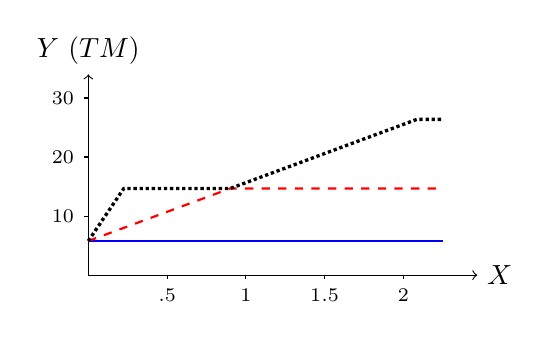
\begin{tikzpicture}[x=2cm,y=.075cm]
\draw[->] (0,0)--(2.47,0) node[right] {$X$};
\draw[->] (0,0)--(0,34) node[above] {$Y\ (TM)$};
\foreach \a in {.5,1,1.5,2} {\draw (\a,0)--(\a,-.7) node[below,font=\scriptsize] {$\a$};}
\foreach \a in {10,20,30} {\draw (0,\a)--(-.03,\a) node[left,font=\scriptsize] {$\a$};}
\draw[blue,thick] (0.0000000,5.7831860)--(2.2500000,5.7831860);
\draw[red,dashed,thick] (0.0000000,5.7831860)--(0.9016354,14.6819706)--(2.2500000,14.6819706);
\draw[black,densely dotted,very thick] (0.0000000,5.7831860)--(0.2254088,14.6819706)--(0.9016354,14.6819706)--(2.0863481,26.3746164)--(2.2500000,26.3746164);
\end{tikzpicture}\hspace{.35cm}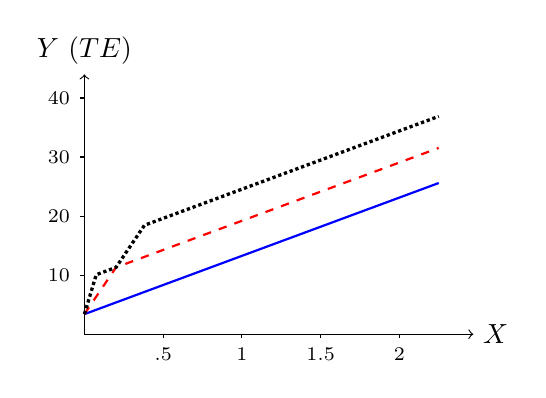
\begin{tikzpicture}[x=2cm,y=.075cm]
\draw[->] (0,0)--(2.47,0) node[right] {$X$};
\draw[->] (0,0)--(0,44) node[above] {$Y\ (TE)$};
\foreach \a in {.5,1,1.5,2} {\draw (\a,0)--(\a,-.7) node[below,font=\scriptsize] {$\a$};}
\foreach \a in {10,20,30,40} {\draw (0,\a)--(-.03,\a) node[left,font=\scriptsize] {$\a$};}
\draw[blue,thick] (0.0000000,3.3899577)--(2.2500000,25.5965676);
\draw[red,dashed,thick] (0.0000000,3.3899577)--(0.2005621,11.3078317)--(2.2500000,31.5349731);
\draw[black,densely dotted,very thick] (0.0000000,3.3899577)--(0.0752108,10.0706639)--(0.2005621,11.3078317)--(0.3813734,18.4459750)--(2.2500000,36.8885805);
\end{tikzpicture}
\end{center}
The transverse ordering used above can also be checked without
surveying indefinitely many roots. The radial eigenvalues for given
$m$ are the min--max values of the Rayleigh quotient
$\int_0^a(|P'|^2+m^2|P|^2/\rho^2)\rho\,d\rho\big/\int_0^a|P|^2\rho\,d\rho$.
Increasing $m^2$ increases the nonnegative term
$m^2\int |P|^2d\rho/\rho$, so each radial eigenvalue increases with
$m$; each fixed-$m$ sequence increases with its radial index.
For TM, the third-lowest value is at most $C$, since $A$, $B$, $C$
are all modes. Every other branch has either $n\ge2$, so
$\alpha_{mn}\ge\alpha_{02}=5.520078$, or $n=1$ and $m\ge3$, so
$\alpha_{m1}\ge\alpha_{31}=6.380162$. Both exceed
$\alpha_{21}=5.135622$, so these branches lie above $C$.
For TE, the zero Neumann eigenvalue is excluded as in
Exercise~14.1.25, and the third-lowest value is at most $F+\pi^2X$.
Every other branch has $n=1$ and $m\ge3$, so
$\beta_{m1}\ge\beta_{31}=4.201189$, or $n\ge2$, so
$\beta_{0n}\ge\beta_{02}>\beta_{01}$ and, for $m\ge1$,
$\beta_{mn}\ge\beta_{12}=5.331443$. All exceed $\beta_{01}$, so with
$p\ge1$ these branches lie above $F+\pi^2X$. In all
these labels $n=1$ means the first \emph{positive} root; in
particular $\beta_{01}=3.831706$, not zero.

\Needspace{5\baselineskip}
\par\bigskip
\noindent\textbf{14.1.28}\quad Show that the integral
\[
\int_{0}^{a}x^{m}J_{n}(x)\,dx,\quad m\ge n\ge0,
\]
\begin{enumerate}
\item[(a)] is integrable for $m+n$ odd in terms of Bessel functions and
powers of $x$, i.e., is expressible as linear combinations of
$a^{p}J_{q}(a)$;
\item[(b)] may be reduced for $m+n$ even to integrated terms plus
$\displaystyle\int_{0}^{a}J_{0}(x)\,dx$.
\end{enumerate}
\par\erratum{Here $m,n$ are nonnegative integers with $m\ge n$.}
\solution
The parity language presumes nonnegative integer $m,n$. Define
$I_{m,n}(a)=\int_0^a x^mJ_n(x)dx$. Since
$[x^{n+1}J_{n+1}(x)]'=x^{n+1}J_n(x)$, integration by parts gives
\begin{align*}
I_{m,n}
&=\int_0^a x^{m-n-1}\,d[x^{n+1}J_{n+1}(x)]\\
&=a^mJ_{n+1}(a)-(m-n-1)I_{m-1,n+1}(a).
\tag{*}
\end{align*}
Explicitly, for $x>0$ the product rule gives
\[
\frac d{dx}\bigl[x^mJ_{n+1}\bigr]
=\frac d{dx}\bigl[x^{m-n-1}\cdot x^{n+1}J_{n+1}\bigr]
=(m-n-1)x^{m-1}J_{n+1}+x^mJ_n,
\]
and integrating from $0$ to $a$ gives (*) for every $m\ge1$, $n\ge0$,
including $m-n-1<0$, which occurs in (b).
The lower boundary term is zero because
$x^mJ_{n+1}(x)=O(x^{m+n+1})$. Every repetition decreases the
power by one, increases the order by one, and leaves their sum
$N=m+n$ unchanged.

(a) If $N$ is odd, then $m-n$ is odd. After $r$ repetitions the
indices are $(m-r,n+r)$, and the next coefficient in (*) is
$(m-r)-(n+r)-1=m-n-1-2r$. After $r=(m-n-1)/2$ repetitions the
remaining indices therefore satisfy $m-r=(n+r)+1$, and at that stage
the coefficient of the remaining integral in (*) is zero. Thus the
procedure ends with the antiderivative $I_{j+1,j}=a^{j+1}J_{j+1}(a)$,
$j=n+r$, and all earlier terms are constants times
$a^{m-r}J_{n+r+1}(a)$. For example, $m-n-1=2$ for $I_{n+3,n}$, so
\[
I_{n+3,n}=a^{n+3}J_{n+1}(a)-2I_{n+2,n+1}
=a^{n+3}J_{n+1}(a)-2a^{n+2}J_{n+2}(a).
\]
This supplies a finite constructive expression of the required type.

(b) If $N$ is even, each coefficient $m-n-1-2r$ in (*) is odd
and cannot vanish. Continue until the power becomes zero, i.e.,
$m$ repetitions, after which the order is $n+m=N$. All the
terms already integrated have the desired form, and only a constant
multiple of $I_{0,N}$ remains. For even $N=2h$, the recurrence
$J_{2j}=J_{2j-2}-2J_{2j-1}'$ (Eq.~(14.8) with $n=2j-1$), integrated
from $0$ to $a$ with $J_{2j-1}(0)=0$, gives
$I_{0,2j}=I_{0,2j-2}-2J_{2j-1}(a)$; applying this for
$j=h,h-1,\ldots,1$,
\begin{align*}
I_{0,2h}(a)
&=I_{0,2h-2}(a)-2J_{2h-1}(a)\\
&=\boxed{\int_0^a J_0(x)dx-2\sum_{j=1}^{h}J_{2j-1}(a)}.
\end{align*}
All odd-order Bessel functions vanish at zero, so no omitted lower
boundary constants occur. Inserting this into the repeated formula
(*) proves the requested reduction.

\Needspace{5\baselineskip}
\par\bigskip
\noindent\textbf{14.1.29}\quad Show that
\[
\int_{0}^{\alpha_{0n}}\left(1-\frac{y}{\alpha_{0n}}\right)J_{0}(y)y\,dy
=\frac{1}{\alpha_{0n}}\int_{0}^{\alpha_{0n}}J_{0}(y)\,dy.
\]
Here $\alpha_{0n}$ is the $n$th zero of $J_{0}(y)$. This relation is
useful (see Exercise~14.2.9): The expression on the right is easier
and quicker to evaluate, and is much more accurate. Taking the
difference of two terms in the expression on the left leads to a large
relative error.
\solution
Set $A=\alpha_{0n}>0$, so $J_0(A)=0$. First use
$[yJ_1(y)]'=yJ_0(y)$:
\begin{align*}
\int_0^A(1-y/A)yJ_0(y)dy
&=\left[(1-y/A)yJ_1(y)\right]_0^A
+\frac1A\int_0^A yJ_1(y)dy\\
&=\frac1A\int_0^A yJ_1(y)dy.
\end{align*}
The upper boundary vanishes because $1-A/A=0$, and the lower
boundary because $yJ_1(y)=O(y^2)$. Now $J_1=-J_0'$ and a second
integration by parts gives
\begin{align*}
\frac1A\int_0^A yJ_1(y)dy
&=-\frac1A[yJ_0(y)]_0^A+\frac1A\int_0^A J_0(y)dy\\
&=\boxed{\frac1A\int_0^A J_0(y)dy}.
\end{align*}
The last boundary term is zero by the defining root condition.
The identity avoids separately evaluating the two oscillatory
moments $\int yJ_0$ and $A^{-1}\int y^2J_0$ and then subtracting
them; the smaller final quantity is computed directly.

\Needspace{9\baselineskip}
\subsection*{14.2 Orthogonality}

\Needspace{5\baselineskip}
\par\bigskip
\noindent\textbf{14.2.1}\quad Show that
\[
\int_{0}^{a}J_{\nu}(kx)J_{\nu}(k'x)x\,dx
=\frac{a[k'J_{\nu}(ka)J'_{\nu}(k'a)-kJ'_{\nu}(ka)J_{\nu}(k'a)]}
{(k^{2}-k'^{2})},
\]
where $J'_{\nu}(ka)=\dfrac{d}{d(kx)}J_{\nu}(kx)\Big|_{x=a}$, and that
\[
\int_{0}^{a}[J_{\nu}(kx)]^{2}x\,dx
=\frac{a^{2}}{2}\left\{[J'_{\nu}(ka)]^{2}
+\left(1-\frac{\nu^{2}}{k^{2}a^{2}}\right)[J_{\nu}(ka)]^{2}\right\},
\qquad\nu>-1.
\]
These two integrals are usually called the first and second Lommel
integrals.
\par\erratum{Take real $\nu>-1$, $a>0$, and $k,k'>0$. The first displayed quotient requires $k^2\ne k'^2$; its coincident limit is the second integral.}
\solution
Let $y(x)=J_\nu(kx)$ and $z(x)=J_\nu(k'x)$, initially with
$k,k'>0$, $k^2\ne k'^2$. Their equations in self-adjoint form are
\[
(xy')'+(k^2x-\nu^2/x)y=0,\qquad
(xz')'+(k'^2x-\nu^2/x)z=0.
\]
Multiply the second by $y$, the first by $z$, and subtract:
\[
\frac d{dx}\{x(yz'-y'z)\}=(k^2-k'^2)xyz.
\]
Integrate first from $\epsilon>0$ to $a$, so no individually
divergent origin terms have been introduced. To take $\epsilon\to0$,
write
\[
y=A x^\nu\left[1-\frac{k^2x^2}{4(\nu+1)}+O(x^4)\right],\quad
z=B x^\nu\left[1-\frac{k'^2x^2}{4(\nu+1)}+O(x^4)\right].
\]
The leading powers cancel in the bracket, leaving
\[
x(yz'-y'z)=\frac{AB(k^2-k'^2)}{2(\nu+1)}x^{2\nu+2}
+O(x^{2\nu+4})\longrightarrow0\qquad(\nu>-1).
\]
At $a$, the chain rule gives $y'=kJ_\nu'(ka)$ and
$z'=k'J_\nu'(k'a)$. Hence
\[
\boxed{\int_0^a xyz\,dx=
\frac{a[k'J_\nu(ka)J_\nu'(k'a)-kJ_\nu'(ka)J_\nu(k'a)]}
{k^2-k'^2}}.
\]
For the second integral let $k'\to k$ and apply l'H\^opital's rule.
Writing $J=J_\nu(ka)$ and using primes for argument derivatives,
\[
\int_0^a xJ_\nu(kx)^2dx
=\frac{a[J(J'+kaJ'')-ka(J')^2]}{-2k}.
\]
Bessel's equation at $ka$ says
$kaJ''=-J'-(ka-\nu^2/(ka))J$. Therefore
\[
J(J'+kaJ'')-ka(J')^2
=-ka\left[(J')^2+\left(1-\frac{\nu^2}{k^2a^2}\right)J^2\right],
\]
which gives
\[
\boxed{\int_0^a xJ_\nu(kx)^2dx
=\frac{a^2}{2}\left[J_\nu'(ka)^2+
\left(1-\frac{\nu^2}{k^2a^2}\right)J_\nu(ka)^2\right]}.
\]
The condition $\nu>-1$ also makes the integrand
$O(x^{2\nu+1})$ integrable. Coincident wave numbers use the second
formula; any zero-parameter value must be taken as an existing
limit, not inserted into the displayed denominators.

\Needspace{5\baselineskip}
\par\bigskip
\noindent\textbf{14.2.2}
\begin{enumerate}
\item[(a)] If $\beta_{\nu m}$ is the $m$th \erratum{positive zero of $J_\nu^\prime$}, so that
\erratum{$(d/d\rho)J_\nu(\beta_{\nu m}\rho/a)|_{\rho=a}=0$}, show that the Bessel functions
are orthogonal over the interval $[0,a]$ with an orthogonality
integral
\[
\int_{0}^{a}J_{\nu}\left(\beta_{\nu m}\frac{\rho}{a}\right)
J_{\nu}\left(\beta_{\nu n}\frac{\rho}{a}\right)\rho\,d\rho=0,
\qquad m\neq n,\quad\nu>-1.
\]
\item[(b)] Derive the corresponding normalization integral ($m=n$).
\end{enumerate}
\par\nobreak\hfill\emph{ANS.}\enspace
(b) $\dfrac{a^{2}}{2}\left(1-\dfrac{\nu^{2}}{\beta_{\nu m}^{2}}\right)
[J_{\nu}(\beta_{\nu m})]^{2}$, $\nu>-1$.
\par\erratum{These formulas refer to positive derivative roots. For $\nu=0$ the additional constant mode has norm $a^2/2$.}
\solution
Interpret $\beta_{\nu m}$ as a positive argument satisfying
$J_\nu'(\beta_{\nu m})=0$, so the derivative with respect to $\rho$
vanishes at $\rho=a$. Put $k=\beta_{\nu m}/a$ and
$k'=\beta_{\nu n}/a$ in the first Lommel integral. For $m\ne n$
the denominator is nonzero, while both terms in its numerator
contain a vanishing derivative. Thus
\[
\boxed{\int_0^a \rho J_\nu(\beta_{\nu m}\rho/a)
J_\nu(\beta_{\nu n}\rho/a)d\rho=0\quad(m\ne n)}.
\]
For $m=n$, use the second Lommel integral instead. The squared
derivative term is zero, and $k^2a^2=\beta_{\nu m}^2$, giving
\[
\boxed{N_{\nu m}=\frac{a^2}{2}
\left(1-\frac{\nu^2}{\beta_{\nu m}^2}\right)
J_\nu(\beta_{\nu m})^2}.
\]
The origin terms vanish for $\nu>-1$ by the calculation in
Exercise~14.2.1. The integral defining $N_{\nu m}$ is positive,
so this also implies $\beta_{\nu m}>|\nu|$ for every positive
derivative zero under consideration.
\erratum{For $\nu=0$ the Neumann problem has the additional
constant mode $J_0(0\rho/a)=1$, of norm $a^2/2$. It is not one
of the positive roots, and the displayed expression containing
$\nu^2/\beta^2$ must not be used as $0/0$. Its orthogonality to
the positive modes follows from
$\int_0^a\rho J_0(\beta\rho/a)d\rho=a^2J_1(\beta)/\beta=0$.}

\Needspace{5\baselineskip}
\par\bigskip
\noindent\textbf{14.2.3}\quad Verify that the orthogonality equation,
Eq.~(14.44), and the normalization equation, Eq.~(14.46), hold for
$\nu>-1$.
\par\emph{Hint.}~Using power-series expansions, examine the behavior of
Eq.~(14.43) as $\rho\to0$.
\solution
The two equations to be checked are the Dirichlet orthogonality
and normalization formulas
\[
\int_0^a\rho J_\nu(\alpha_{\nu m}\rho/a)
J_\nu(\alpha_{\nu n}\rho/a)d\rho=0\quad(m\ne n),
\]
\[
\int_0^a\rho J_\nu(\alpha_{\nu n}\rho/a)^2d\rho
=\frac{a^2}{2}J_{\nu+1}(\alpha_{\nu n})^2.
\]
The only possible issue when $-1<\nu<0$ is the singular-looking
origin. Put $k=\alpha_{\nu m}/a$, $k'=\alpha_{\nu n}/a$.
The series begin
\[
J_\nu(k\rho)=\frac{(k/2)^\nu}{\Gamma(\nu+1)}\rho^\nu
\left[1-\frac{k^2\rho^2}{4(\nu+1)}+O(\rho^4)\right].
\]
In the boundary expression
$\rho[J_\nu(k\rho)\partial_\rho J_\nu(k'\rho)
-\partial_\rho J_\nu(k\rho)J_\nu(k'\rho)]$, the terms of order
$\rho^{2\nu}$ cancel exactly. The next term is
\[
\frac{(kk'/4)^\nu(k^2-k'^2)}
{2(\nu+1)\Gamma(\nu+1)^2}\rho^{2\nu+2},
\]
which vanishes for precisely the stated range $\nu>-1$.
At $\rho=a$ both function values vanish for distinct Dirichlet
roots, so the first Lommel formula gives orthogonality. For a
repeated root, the second formula reduces to
$a^2J_\nu'(\alpha_{\nu n})^2/2$. The recurrence
$J_\nu'=\nu J_\nu/x-J_{\nu+1}$ yields
$J_\nu'(\alpha_{\nu n})=-J_{\nu+1}(\alpha_{\nu n})$, proving
normalization. All relevant integrals converge because their
origin integrands behave as $\rho^{2\nu+1}$.

\Needspace{5\baselineskip}
\par\bigskip
\noindent\textbf{14.2.4}\quad From Eq.~\erratum{(14.44)}, develop a
proof that $J_{\nu}(z)$, $\nu>-1$ has no complex roots (with a nonzero
imaginary part).
\par\emph{Hint.}
\begin{enumerate}
\item[(a)] Use the series form of $J_{\nu}(z)$ to exclude pure
imaginary roots.
\item[(b)] Assume $\alpha_{\nu m}$ to be complex and take
$\alpha_{\nu n}$ to be $\alpha_{\nu m}^{\,*}$.
\end{enumerate}
\solution
Take real $\nu>-1$ and consider nonzero roots on a fixed
branch. The factor $z^\nu$ can be removed by defining the entire
even function
\[
F_\nu(z)=\Gamma(\nu+1)(2/z)^\nu J_\nu(z)
=\sum_{r=0}^\infty
\frac{(-1)^r\Gamma(\nu+1)(z^2/4)^r}
{r!\Gamma(\nu+r+1)}.
\]
(a) If $z=iy$ with real $y\ne0$, every term of $F_\nu(iy)$
is positive, because $(-1)^r(iy)^{2r}=y^{2r}$ and all gamma
arguments $\nu+r+1$ are positive. Thus $F_\nu(iy)>0$, excluding
nonzero pure imaginary roots.

(b) The series coefficients are real, so if $z_0$ is a root then
$z_0^*$ is also a root. Suppose both its real and imaginary parts
are nonzero. Then $z_0^2\ne(z_0^*)^2$. Apply the first Lommel
identity on $0\le x\le1$ with $k=z_0$, $k'=z_0^*$.
The upper boundary term vanishes because both arguments are roots;
the lower boundary vanishes by the same $x^{2\nu+2}$ estimate as
before. With conjugate branches for the two factors, this says
\[
0=\int_0^1 xJ_\nu(z_0x)J_\nu(z_0^*x)dx
=\int_0^1 x|J_\nu(z_0x)|^2dx.
\]
But the integrand is nonnegative and the series shows that the
function is not identically zero on $(0,1)$, so the integral is
strictly positive. This contradiction excludes every remaining
nonreal possibility. Therefore all nonzero zeros are real.
The corrected reference is Eq.~(14.44), the orthogonality identity;
the original reference to (11.49) is unrelated.

\Needspace{5\baselineskip}
\par\bigskip
\noindent\textbf{14.2.5}
\begin{enumerate}
\item[(a)] In the series expansion
\[
f(\rho)=\sum_{m=1}^{\infty}c_{\nu m}J_{\nu}\left(\alpha_{\nu m}
\frac{\rho}{a}\right),\quad0\le\rho\le a,\quad\nu>-1,
\]
with $J_{\nu}(\alpha_{\nu m})=0$, show that the coefficients are given
by
\[
c_{\nu m}=\frac{2}{a^{2}[J_{\nu+1}(\alpha_{\nu m})]^{2}}
\int_{0}^{a}f(\rho)J_{\nu}\left(\alpha_{\nu m}\frac{\rho}{a}\right)
\rho\,d\rho.
\]
\item[(b)] In the series expansion
\[
f(\rho)=\erratum{f_{\rm extra}(\rho)+}\sum_{m=1}^{\infty}d_{\nu m}J_{\nu}\left(\beta_{\nu m}
\frac{\rho}{a}\right),\quad0\le\rho\le a,\quad\nu>-1,
\]
with $(d/d\rho)J_{\nu}(\beta_{\nu m}\rho/a)\big|_{\rho=a}=0$, show
that the coefficients are given by
\[
d_{\nu m}=\frac{2}{a^{2}(1-\nu^{2}/\beta_{\nu m}^{2})
[J_{\nu}(\beta_{\nu m})]^{2}}
\int_{0}^{a}f(\rho)J_{\nu}\left(\beta_{\nu m}\frac{\rho}{a}\right)
\rho\,d\rho.
\]
\end{enumerate}
\par\erratum{Use real $\nu>-1$ and convergence in $L^2((0,a),\rho\,d\rho)$; the roots are positive. In (b), include $f_{\rm extra}=0$ for $\nu>0$, a constant mode for $\nu=0$, and the mode proportional to $I_\nu(\kappa\rho/a)$ with $I_\nu^\prime(\kappa)=0$ for $-1<\nu<0$. Its coefficient is determined below.}
\solution
Use the weighted inner product
$\langle g,h\rangle=\int_0^a g(\rho)^*h(\rho)\rho\,d\rho$.
The coefficient formulas hold whenever the stated expansions
converge in this weighted $L^2$ space.

(a) Multiply the Dirichlet expansion by
$J_\nu(\alpha_{\nu n}\rho/a)\rho$ and integrate. Orthogonality
removes every term except $m=n$:
\[
\int_0^a f(\rho)J_\nu(\alpha_{\nu n}\rho/a)\rho d\rho
=c_{\nu n}\frac{a^2}{2}J_{\nu+1}(\alpha_{\nu n})^2.
\]
Division gives the asserted $c_{\nu n}$.

(b) Repeat with $J_\nu(\beta_{\nu n}\rho/a)\rho$ instead.
The Neumann orthogonality and norm from Exercise~14.2.2 give
\[
\int_0^a f(\rho)J_\nu(\beta_{\nu n}\rho/a)\rho d\rho
=d_{\nu n}\frac{a^2}{2}
\left(1-\frac{\nu^2}{\beta_{\nu n}^2}\right)
J_\nu(\beta_{\nu n})^2.
\]
Solving for $d_{\nu n}$ proves the second displayed coefficient
formula for each positive root.

\erratum{Positive derivative roots alone do not give an expansion
of an arbitrary function throughout the stated range $\nu>-1$.
For $\nu=0$ one must add the constant mode with coefficient
$d_{00}=2a^{-2}\int_0^a f(\rho)\rho\,d\rho$.
For $-1<\nu<0$ one must also include a negative-eigenvalue mode
$I_\nu(\kappa\rho/a)$, where $I_\nu'(\kappa)=0$, $\kappa>0$.
These omissions do not change the coefficient formulas for the
positive-root terms.}
Here is a direct check of the latter qualification. For $-1<\nu<0$,
$I_\nu(x)>0$ by its series, its derivative is negative near zero
($I_\nu\sim(x/2)^\nu/\Gamma(\nu+1)$), and positive for large
$x$. Thus it has a positive derivative zero. If
$w=xI_\nu'/I_\nu$, the modified Bessel equation gives
$xw'=x^2+\nu^2-w^2$. At every zero of $w$ its derivative is
positive, so it crosses zero only once. The corresponding radial
function has eigenvalue $-\kappa^2/a^2$ and is orthogonal to all
positive-eigenvalue modes by the same boundary-bracket argument.
For clarity, derive its norm rather than assuming a modified Lommel
formula. Put $y(x)=I_\nu(x)$ and
\[
F(x)=\frac12\{x^2[y(x)^2-y'(x)^2]+\nu^2y(x)^2\}.
\]
Differentiation gives
\[
F'=x(y^2-y'^2)+(x^2+\nu^2)yy'-x^2y'y''.
\]
The modified equation says
$x^2y''=(x^2+\nu^2)y-xy'$. Substitution cancels the two
$yy'$ terms and the two $xy'^2$ terms, leaving $F'=xy^2$.
Near zero, the leading $x^{2\nu}$ contributions cancel in $F$,
so $F=O(x^{2\nu+2})\to0$ for $\nu>-1$.
Now set $x=\kappa\rho/a$ and use $I_\nu^\prime(\kappa)=0$:
\[
N_-=\frac{a^2}{\kappa^2}\int_0^\kappa xI_\nu(x)^2\,dx
=\frac{a^2}{\kappa^2}[F(\kappa)-F(0)].
\]
Thus its norm is
\[
N_-=\frac{a^2}{2}\left(1+\frac{\nu^2}{\kappa^2}\right)
I_\nu(\kappa)^2,
\]
so its coefficient is
$N_-^{-1}\int_0^a f(\rho)I_\nu(\kappa\rho/a)\rho d\rho$.
At the Dirichlet endpoint $\rho=a$, a series of zero-valued basis
functions is zero; nonzero prescribed endpoint values are understood
as interior limits or in $L^2$, rather than equality at that single
point.

\Needspace{5\baselineskip}
\par\bigskip
\noindent\textbf{14.2.6}\quad A right circular cylinder has an
electrostatic potential of $\psi(\rho,\varphi)$ on both ends. The
potential on the curved cylindrical surface is zero. Find the
potential at all interior points.
\par\emph{Hint.}~Choose your coordinate system and adjust your $z$
dependence to exploit the symmetry of your potential.
\par\erratum{Assume bounded, piecewise smooth end data, and seek the bounded harmonic interior solution. At an incompatible rim, impose the face limits away from the junction.}
\solution
Let the cylinder have radius $a$ and length $l$, with its ends
at $z=\pm l/2$. Denote the sought interior potential by $V$ and
the identical prescribed end potential by $\psi(\rho,\varphi)$.
Separation of $\nabla^2V=0$ gives the angular factors $e^{im\varphi}$,
regular radial factors $J_{|m|}(k\rho)$, and axial equation
$Z''-k^2Z=0$. The side condition forces
$k=\alpha_{|m|n}/a$, where $J_{|m|}(\alpha_{|m|n})=0$.
Identical end data are even in $z$; hence use $\cosh(kz)$ rather
than the odd $\sinh(kz)$. Normalize the axial factor to one on
both ends:
\[
\boxed{V(\rho,\varphi,z)=\sum_{m=-\infty}^{\infty}
\sum_{n=1}^{\infty}A_{mn}J_{|m|}(\alpha_{|m|n}\rho/a)
e^{im\varphi}
\frac{\cosh(\alpha_{|m|n}z/a)}
{\cosh(\alpha_{|m|n}l/(2a))}}.
\]
At either end this is the double Fourier--Bessel expansion of
$\psi$. Multiply it by
$e^{-im\varphi}J_{|m|}(\alpha_{|m|n}\rho/a)\rho$ and integrate
over the disk. The angular norm is $2\pi$ and the radial norm is
$a^2J_{|m|+1}(\alpha_{|m|n})^2/2$. Therefore
\[
\boxed{A_{mn}=\frac{\displaystyle\int_0^{2\pi}\!\int_0^a
\psi(\rho,\varphi)e^{-im\varphi}
J_{|m|}(\alpha_{|m|n}\rho/a)\rho\,d\rho\,d\varphi}
{\pi a^2J_{|m|+1}(\alpha_{|m|n})^2}}.
\]
Every term satisfies Laplace's equation, the grounded side, and
reflection symmetry; the coefficient projection supplies both end
conditions. For real data $A_{-m,n}=A_{mn}^*$, making the potential
real. For compatible boundary data and finite-energy solutions,
the difference $U=V_1-V_2$ has zero boundary values. Green's
identity gives $\int|\nabla U|^2d^3x=0$, hence $U=0$.

\erratum{A discontinuous rim need not give a finite-energy field,
so that energy argument should not be applied to each such field
without qualification.} Uniqueness still holds among bounded
harmonic solutions with the specified face limits. To see this,
let $\Gamma$ be the two rim circles and introduce the positive
harmonic barrier
\[
B(\mathbf x)=\int_\Gamma\frac{d\ell_{\mathbf y}}{|\mathbf x-\mathbf y|}.
\]
It is finite in the interior, harmonic there, and diverges to
$+\infty$ at the rim: the local line integral is comparable to
$\int_{-\delta}^{\delta}(d^2+s^2)^{-1/2}ds
=2\operatorname{arsinh}(\delta/d)\to\infty$.
For any $\epsilon>0$, both $U-\epsilon B$ and
$-U-\epsilon B$ have nonpositive boundary upper limits, including
the rim because $U$ is bounded. The maximum principle gives
$|U(\mathbf x)|\le\epsilon B(\mathbf x)$ in the interior.
Letting $\epsilon\downarrow0$ proves $U=0$.
The series therefore supplies the bounded interior solution and,
at incompatible rims, the face limits away from the junction.

\Needspace{5\baselineskip}
\par\bigskip
\noindent\textbf{14.2.7}\quad A function $f(x)$ is expressed as a
Bessel series:
\[
f(x)=\sum_{n=1}^{\infty}a_{n}J_{m}(\alpha_{mn}x),
\]
with $\alpha_{mn}$ the $n$th root of $J_{m}$. Prove the Parseval
relation,
\[
\int_{0}^{1}[f(x)]^{2}x\,dx
=\frac{1}{2}\sum_{n=1}^{\infty}a_{n}^{2}[J_{m+1}(\alpha_{mn})]^{2}.
\]
\par\erratum{Let $m>-1$ be real, let $\alpha_{mn}$ enumerate the positive zeros, and assume convergence to $f$ in $L^2((0,1),x\,dx)$.}
\solution
First take a finite partial sum
$S_N(x)=\sum_{n=1}^N a_nJ_m(\alpha_{mn}x)$. Expanding its square,
then using orthogonality and the Dirichlet norm, gives
\begin{align*}
\int_0^1 S_N(x)^2x\,dx
&=\sum_{n=1}^N\sum_{j=1}^N a_na_j
\int_0^1J_m(\alpha_{mn}x)J_m(\alpha_{mj}x)x\,dx\\
&=\frac12\sum_{n=1}^N a_n^2J_{m+1}(\alpha_{mn})^2.
\end{align*}
\erratum{To pass to an infinite series, the expansion must converge
to $f$ in $L^2((0,1),x\,dx)$; merely writing a formal series does
not justify Parseval's equality.}
Under that assumption, the Cauchy--Schwarz inequality gives
\[
\left|\int_0^1(f^2-S_N^2)x\,dx\right|
\le\|f-S_N\|\,\|f+S_N\|\longrightarrow0.
\]
The finite identity therefore tends to the formula in the question.
For real $f$ and coefficients this is the usual Parseval identity.
For complex functions, the norm version is
\[
\int_0^1|f(x)|^2x\,dx
=\frac12\sum_{n=1}^{\infty}|a_n|^2J_{m+1}(\alpha_{mn})^2;
\]
the bilinear square identity also follows by the same limiting
argument. Completeness of the Dirichlet Bessel basis identifies the
limit with $f$, rather than merely its orthogonal projection.

\Needspace{5\baselineskip}
\par\bigskip
\noindent\textbf{14.2.8}\quad Prove that
\[
\sum_{n=1}^{\infty}(\alpha_{mn})^{-2}=\frac{1}{4(m+1)}.
\]
\par\emph{Hint.}~Expand $x^{m}$ in a Bessel series and apply the
Parseval relation.
\par\erratum{Here $m>-1$ is real and $\alpha_{mn}$ is the $n$th positive zero of $J_m$.}
\solution
Expand $f(x)=x^m$ on $0<x<1$ in the Dirichlet Bessel basis.
For $m>-1$, $\int_0^1|x^m|^2x\,dx=1/[2(m+1)]$ is finite.
The coefficient formula gives
\[
a_n=\frac{2}{J_{m+1}(\alpha_{mn})^2}
\int_0^1x^{m+1}J_m(\alpha_{mn}x)dx.
\]
Set $\alpha=\alpha_{mn}$. The recurrence implies
\[
\frac d{dx}[x^{m+1}J_{m+1}(\alpha x)]
=\alpha x^{m+1}J_m(\alpha x).
\]
Its lower boundary vanishes as $x^{2m+2}$; hence
\[
\int_0^1x^{m+1}J_m(\alpha x)dx
=\frac{J_{m+1}(\alpha)}\alpha,
\qquad a_n=\frac{2}{\alpha_{mn}J_{m+1}(\alpha_{mn})}.
\]
Insert these coefficients into Parseval's relation:
\begin{align*}
\frac1{2(m+1)}
&=\frac12\sum_{n=1}^{\infty}
\frac{4J_{m+1}(\alpha_{mn})^2}
{\alpha_{mn}^2J_{m+1}(\alpha_{mn})^2}
=2\sum_{n=1}^{\infty}\alpha_{mn}^{-2}.
\end{align*}
Thus
\[
\boxed{\sum_{n=1}^{\infty}\frac1{\alpha_{mn}^2}
=\frac1{4(m+1)}}.
\]
The expansion is used in the weighted $L^2$ sense. At $x=1$ every
basis function is zero whereas $x^m=1$; that single endpoint has
zero measure and does not affect the integral or Parseval's
identity.

\Needspace{5\baselineskip}
\par\bigskip
\noindent\textbf{14.2.9}\quad A right circular cylinder of length $l$
and radius $a$ has on its end caps a potential
\[
\psi\Big|_{z=\pm\frac{l}{2}}=100\left(1-\frac{\rho}{a}\right).
\]
The potential on the curved surface (the side) is zero. Using the
Bessel series from Exercise~14.2.6, calculate the electrostatic
potential for $\rho/a=0.0(0.2)1.0$ and $z/l=0.0(0.1)0.5$. Take
$a/l=0.5$.
\par\emph{Hint.}~From Exercise~14.1.29 you have
\[
\int_{0}^{\alpha_{0n}}\left(1-\frac{y}{\alpha_{0n}}\right)J_{0}(y)y\,dy.
\]
Show that this equals
\[
\frac{1}{\alpha_{0n}}\int_{0}^{\alpha_{0n}}J_{0}(y)\,dy.
\]
Numerical evaluation of this latter form rather than the former is
both faster and more accurate.
\par\emph{Note.}~For $\rho/a=0.0$ and $z/l=0.5$ the convergence is
slow, 20 terms giving only 98.4 rather than 100.
\par\nobreak\hfill\emph{Check value.}\enspace
For $\rho/a=0.4$ and $z/l=0.3$, $\psi=\erratum{24.559}$.
\solution
The end data are independent of $\varphi$, so only $m=0$ remains
in Exercise~14.2.6. Put $r=\rho/a$, $s=z/l$, and
$\alpha_n=\alpha_{0n}$. Since $l/(2a)=1$,
\[
\boxed{V(r,s)=\sum_{n=1}^{\infty}A_nJ_0(\alpha_n r)
\frac{\cosh(2\alpha_n s)}{\cosh\alpha_n}},
\qquad
A_n=\frac{200}{J_1(\alpha_n)^2}
\int_0^1(1-r)J_0(\alpha_n r)r\,dr.
\]
With $y=\alpha_n r$, the last integral is
\[
\frac1{\alpha_n^2}\int_0^{\alpha_n}
(1-y/\alpha_n)yJ_0(y)dy
=\frac1{\alpha_n^3}\int_0^{\alpha_n}J_0(y)dy,
\]
where the final equality is proved by the two integrations by
parts in Exercise~14.1.29. Consequently the stable coefficients are
\[
\boxed{A_n=\frac{200}{\alpha_n^3J_1(\alpha_n)^2}
\int_0^{\alpha_n}J_0(y)dy}.
\]
\Needspace{12\baselineskip}
The resulting potentials are:
\begin{center}
\begin{tabular}{c r r r r r r}
\toprule
$\rho/a\backslash z/l$ & $0.0$ & $0.1$ & $0.2$ & $0.3$ & $0.4$ & $0.5$\\
\midrule
0.0 & 14.108 & 15.805 & 21.353 & 32.341 & 52.640 & 100.000 \\
0.2 & 13.290 & 14.881 & 20.061 & 30.213 & 48.293 & 80.000 \\
0.4 & 10.989 & 12.287 & 16.485 & 24.559 & 38.270 & 60.000 \\
0.6 & 7.617 & 8.504 & 11.359 & 16.786 & 25.844 & 40.000 \\
0.8 & 3.747 & 4.179 & 5.568 & 8.204 & 12.648 & 20.000 \\
1.0 & 0.000 & 0.000 & 0.000 & 0.000 & 0.000 & 0.000 \\
\bottomrule
\end{tabular}
\end{center}
The last column is the prescribed boundary value $100(1-r)$;
the last row is the grounded side. For the interior entries, the
integrals were accumulated between consecutive zeros of $J_0$,
and 120 modes were summed. Comparing 80 and 120 modes changed
every interior entry by less than $10^{-20}$, comfortably below
the $0.001$ displayed precision. This convergence comparison is a
numerical check, not a universal truncation-error theorem.
\erratum{The printed check value $24.558$ is not correctly rounded
to three decimals: the converged value is
$V(0.4,0.3)=24.5585639709\ldots$, hence $24.559$.}
At the top center, a 20-mode sum is $98.424595978\ldots$; prescribing
the exact boundary value avoids reporting its slowly convergent
truncation as the boundary potential. Symmetry gives
$V(r,-s)=V(r,s)$ for the lower half of the cylinder.

\Needspace{9\baselineskip}
\subsection*{14.3 Neumann Functions, Bessel Functions of the Second Kind}

\Needspace{5\baselineskip}
\par\bigskip
\noindent\textbf{14.3.1}\quad Prove that the Neumann functions $Y_{n}$
(with $n$ an integer) satisfy the recurrence relations
\begin{align*}
Y_{n-1}(x)+Y_{n+1}(x)&=\frac{2n}{x}Y_{n}(x),\\
Y_{n-1}(x)-Y_{n+1}(x)&=2Y'_{n}(x).
\end{align*}
\par\emph{Hint.}~These relations may be proved by differentiating the
recurrence relations for $J_{\nu}$ or by using the limit form of
$Y_{\nu}$ but not dividing everything by zero.
\solution
Begin with noninteger $\nu$, where the defining denominator is
nonzero. Abbreviate $C=\cos\pi\nu$ and $S=\sin\pi\nu$.
Since $\cos\pi(\nu\pm1)=-C$ and $\sin\pi(\nu\pm1)=-S$,
\[
Y_{\nu-1}=\frac{CJ_{\nu-1}+J_{-\nu+1}}S,\qquad
Y_{\nu+1}=\frac{CJ_{\nu+1}+J_{-\nu-1}}S.
\]
Add these and apply the $J$ recurrence at both orders $\nu$ and
$-\nu$:
\begin{align*}
Y_{\nu-1}+Y_{\nu+1}
&=\frac{C(2\nu J_\nu/x)-2\nu J_{-\nu}/x}S
=\frac{2\nu}{x}\frac{CJ_\nu-J_{-\nu}}S
=\frac{2\nu}{x}Y_\nu.
\end{align*}
Subtracting instead gives
\begin{align*}
Y_{\nu-1}-Y_{\nu+1}
&=\frac{C(J_{\nu-1}-J_{\nu+1})
 +(J_{-\nu+1}-J_{-\nu-1})}S\\
&=\frac{2CJ_\nu'-2J_{-\nu}'}S=2Y_\nu'.
\end{align*}
Now let $\nu\to n$. The defining removable limits give
$Y_\nu\to Y_n$, $Y_{\nu\pm1}\to Y_{n\pm1}$, and the same
limits hold after $x$ differentiation away from the branch point
$x=0$. Both recurrences therefore hold for integer $n$, with no
division by $\sin\pi n=0$.

\Needspace{5\baselineskip}
\par\bigskip
\noindent\textbf{14.3.2}\quad Show that for integer $n$
\[
Y_{-n}(x)=(-1)^{n}Y_{n}(x).
\]
\solution
For noninteger $\nu$, solve the definition for the opposite-order
first-kind function:
\[
J_{-\nu}=\cos\pi\nu\,J_\nu-\sin\pi\nu\,Y_\nu.
\]
Apply the definition once more with order $-\nu$:
\begin{align*}
Y_{-\nu}
&=\frac{\cos\pi\nu\,J_{-\nu}-J_\nu}{-\sin\pi\nu}\\
&=\frac{(\cos^2\pi\nu-1)J_\nu
-\cos\pi\nu\sin\pi\nu\,Y_\nu}{-\sin\pi\nu}\\
&=\sin\pi\nu\,J_\nu+\cos\pi\nu\,Y_\nu.
\end{align*}
Taking the removable limit $\nu\to n\in\mathbb Z$ gives
\[
\boxed{Y_{-n}(x)=(-1)^nY_n(x)}.
\]
This also includes $n=0$, where the equality is immediate.

\Needspace{5\baselineskip}
\par\bigskip
\noindent\textbf{14.3.3}\quad Show that
\[
Y'_{0}(x)=-Y_{1}(x).
\]
\solution
Set $n=0$ in the derivative recurrence:
\[
2Y_0'=Y_{-1}-Y_1.
\]
Exercise~14.3.2 gives $Y_{-1}=-Y_1$, and hence
\[
2Y_0'=-2Y_1,\qquad\boxed{Y_0'=-Y_1}.
\]
\erratum{The manual's last equation in this exercise, p.~209,
prints $J_1,J_0'$ where $Y_1,Y_0'$ are required. The latter are
the functions used in the recurrence above.}

\Needspace{5\baselineskip}
\par\bigskip
\noindent\textbf{14.3.4}\quad If $X$ and $Z$ are any two solutions of
Bessel's equation, show that
\[
X_{\nu}(x)Z'_{\nu}(x)-X'_{\nu}(x)Z_{\nu}(x)=\frac{A_{\nu}}{x},
\]
in which $A_{\nu}$ may depend on $\nu$ but is independent of $x$. This
is a special case of Exercise~7.6.11.
\solution
Define $W=X_\nu Z_\nu'-X_\nu'Z_\nu$ on an interval not
containing $x=0$. Differentiation cancels the mixed terms:
\[
W'=X_\nu Z_\nu''-X_\nu''Z_\nu.
\]
Both functions satisfy
$y''=-y'/x-(1-\nu^2/x^2)y$. Substitution therefore gives
\begin{align*}
W'&=X_\nu\left[-\frac{Z_\nu'}x-
\left(1-\frac{\nu^2}{x^2}\right)Z_\nu\right]
-\left[-\frac{X_\nu'}x-
\left(1-\frac{\nu^2}{x^2}\right)X_\nu\right]Z_\nu\\
&=-\frac1x(X_\nu Z_\nu'-X_\nu'Z_\nu)=-\frac Wx.
\end{align*}
Thus $(xW)'=W+xW'=0$, proving
\[
\boxed{W(x)=\frac{A_\nu}{x}}.
\]
The constant depends on the chosen solutions and their order, but
not on $x$. It is zero for linearly dependent solutions.

\Needspace{5\baselineskip}
\par\bigskip
\noindent\textbf{14.3.5}\quad Verify the Wronskian formulas
\begin{align*}
J_{\nu}(x)J_{-\nu+1}(x)+J_{-\nu}(x)J_{\nu-1}(x)
&=\frac{2\sin\nu\pi}{\pi x},\\
J_{\nu}(x)Y'_{\nu}(x)-J'_{\nu}(x)Y_{\nu}(x)&=\frac{2}{\pi x}.
\end{align*}
\solution
For noninteger $\nu$, the derivative recurrences give
\[
J_{1-\nu}=-J_{-\nu}'-\frac\nu xJ_{-\nu},\qquad
J_{\nu-1}=J_\nu'+\frac\nu xJ_\nu.
\]
Multiplying and adding cancels the terms proportional to $\nu/x$:
\[
J_\nu J_{1-\nu}+J_{-\nu}J_{\nu-1}
=-J_\nu J_{-\nu}'+J_\nu'J_{-\nu}
=-W[J_\nu,J_{-\nu}].
\]
\erratum{The manual's corresponding line on p.~209 has a minus
sign before the second product; it must be plus, as the cancellation
above shows.}
By Exercise~14.3.4, $W=A/x$. The leading series terms are
\[
J_\nu=\frac{(x/2)^\nu}{\Gamma(\nu+1)}[1+O(x^2)],\qquad
J_{-\nu}=\frac{(x/2)^{-\nu}}{\Gamma(1-\nu)}[1+O(x^2)].
\]
Their derivatives give
\[
A=-\frac{2\nu}{\Gamma(\nu+1)\Gamma(1-\nu)}
=-\frac{2}{\Gamma(\nu)\Gamma(1-\nu)}
=-\frac{2\sin\pi\nu}{\pi}.
\]
Therefore
\[
\boxed{J_\nu J_{1-\nu}+J_{-\nu}J_{\nu-1}
=\frac{2\sin\pi\nu}{\pi x}}.
\]
Finally $Y_\nu=(\cos\pi\nu\,J_\nu-J_{-\nu})/\sin\pi\nu$,
so bilinearity of the Wronskian gives
\[
W[J_\nu,Y_\nu]=-
\frac{W[J_\nu,J_{-\nu}]}{\sin\pi\nu}
=\boxed{\frac2{\pi x}}.
\]
Both formulas extend to integer orders by their removable order
limits. In the first, both sides then vanish because $J_{-n}$ is
proportional to $J_n$; the second remains nonzero.

\Needspace{5\baselineskip}
\par\bigskip
\noindent\textbf{14.3.6}\quad As an alternative to letting $x$ approach
zero in the evaluation of the Wronskian constant, we may invoke the
uniqueness of power-series expansions. The coefficient of $x^{-1}$ in
the series expansion of $u_{\nu}(x)v'_{\nu}(x)-u'_{\nu}(x)v_{\nu}(x)$
is then $A_{\nu}$. Show by series expansion that the coefficients of
$x^{0}$ and $x^{1}$ of
$J_{\nu}(x)J'_{-\nu}(x)-J'_{\nu}(x)J_{-\nu}(x)$ are each zero.
\solution
For noninteger $\nu$, write the first two series terms as
\[
J_\nu=A x^\nu(1-ax^2+O(x^4)),\quad
J_{-\nu}=B x^{-\nu}(1-bx^2+O(x^4)),
\]
where
\[
A=\frac{2^{-\nu}}{\Gamma(\nu+1)},\quad
B=\frac{2^\nu}{\Gamma(1-\nu)},\quad
a=\frac1{4(\nu+1)},\quad b=\frac1{4(1-\nu)}.
\]
All powers in either product $J_\nu J_{-\nu}'$ or
$J_\nu'J_{-\nu}$ are $x^{2r-1}$ with integer $r\ge0$.
Consequently an $x^0$ term cannot occur. For $x^1$, differentiate
the two displayed series and multiply:
\begin{align*}
J_\nu J_{-\nu}'
&=AB\left[-\frac\nu x+
\{a\nu-b(2-\nu)\}x+O(x^3)\right],\\
J_\nu'J_{-\nu}
&=AB\left[\frac\nu x+
\{-b\nu-a(\nu+2)\}x+O(x^3)\right].
\end{align*}
Subtracting, the $x$ coefficient is
\[
2AB[(\nu+1)a+(\nu-1)b]
=2AB\left[\frac14-\frac14\right]=0.
\]
Thus both requested coefficients vanish, leaving
$-2\nu AB/x+O(x^3)$ at this order. At integer $\nu=n$ the
negative-order relation makes the entire Wronskian identically
zero, so the same coefficient conclusion holds there without
using intermediate gamma factors at their poles.

\Needspace{5\baselineskip}
\par\bigskip
\noindent\textbf{14.3.7}
\begin{enumerate}
\item[(a)] By differentiating and substituting into Bessel's ODE for
$\nu=0$, show that $\displaystyle\int_{0}^{\infty}\cos(x\cosh t)\,dt$
is a solution.
\par\emph{Hint.}~Rearrange the final integral to
$\displaystyle\int_{0}^{\infty}\frac{d}{dt}
\big[x\sin(x\cosh t)\sinh t\big]\,dt$.
\item[(b)] Show that
$Y_{0}(x)=-\dfrac{2}{\pi}\displaystyle\int_{0}^{\infty}
\cos(x\cosh t)\,dt$ is linearly independent of $J_{0}(x)$.
\end{enumerate}
\par\erratum{Take $x>0$. Justify differentiation through an upper-half-plane convergence factor before taking its real-axis boundary limit.}
\solution
\erratum{For real $x>0$, the integral is conditionally convergent.
Its formal $x$ derivatives are not convergent ordinary improper
integrals, and the proposed boundary term
$x\sin(x\cosh t)\sinh t$ does not vanish as $t\to\infty$.
The manual's unregularized integration by parts on p.~211 therefore
needs the limiting argument below.}

(a) Begin in the upper half-plane, with
\[
H(z)=\int_0^\infty e^{iz\cosh t}dt,\qquad\Im z>0.
\]
The factor $e^{-\Im z\cosh t}$ makes the integral and all local
$z$ derivatives absolutely convergent. Direct differentiation gives
\begin{align*}
z^2H''+zH'+z^2H
&=\int_0^\infty[-z^2\sinh^2t+iz\cosh t]e^{iz\cosh t}dt\\
&=\int_0^\infty\frac d{dt}
\left[iz\sinh t\,e^{iz\cosh t}\right]dt=0.
\end{align*}
At $t=0$ the bracket is zero, and at infinity exponential damping
overcomes $\sinh t$. Thus $H$ solves the order-zero Bessel equation.
Its coefficients are analytic near every positive real $x$, so its
solutions continue analytically across that regular part of the
axis. Equivalently, write $H$ locally as a linear combination of
the analytic solutions $J_0$ and $Y_0$ and continue those functions.

Now put $u=\cosh t$. The real part of the boundary value is
\[
F(x)=\int_1^\infty\frac{\cos(xu)}{\sqrt{u^2-1}}du
=\int_0^\infty\cos(x\cosh t)dt.
\]
The singularity at $u=1$ is integrable and the tail converges by
Dirichlet's test. Abel convergence therefore identifies it with
$\lim_{\epsilon\downarrow0}\Re H(x+i\epsilon)$. The analytic
continuation just established makes this limit a smooth solution:
\[
\boxed{x^2F''+xF'+x^2F=0\quad(x>0)}.
\]

(b) To compare it with $J_0$, split off an elementary logarithmic
integral:
\[
F(x)=\int_1^\infty\frac{\cos(xu)}u\,du
+\int_1^\infty\cos(xu)
\left(\frac1{\sqrt{u^2-1}}-\frac1u\right)du.
\]
The first is $-\operatorname{Ci}(x)=-\gamma-\ln x+o(1)$.
The difference in parentheses is absolutely integrable; dominated
convergence gives for the second integral
\[
\lim_{R\to\infty}[\operatorname{arcosh}R-\ln R]=\ln2.
\]
Consequently
\[
-\frac2\pi F(x)=\frac2\pi[\ln(x/2)+\gamma]+o(1).
\]
This diverges logarithmically as $x\downarrow0$, whereas $J_0(x)$
tends to one. They are linearly independent. The logarithmic
coefficient and constant also agree with the defining series of
$Y_0$; a difference of two such solutions would be a multiple of
$J_0$ tending to zero, so that multiple is zero. Hence
$Y_0(x)=-2F(x)/\pi$ with the stated normalization.

\Needspace{5\baselineskip}
\par\bigskip
\noindent\textbf{14.3.8}\quad Verify the expansion formula for $Y_{n}(x)$
given in Eq.~(14.61).
\par\emph{Hint.}~Start from Eq.~(14.60) and perform the indicated
differentiations on the power-series expansions of $J_{\nu}$ and
$J_{-\nu}$. The digamma functions $\psi$ arise from the
differentiation of the gamma function. You will need the identity (not
derived in this book)
$\displaystyle\lim_{z\to-n}\psi(z)/\Gamma(z)=(-1)^{n-1}n!$, where $n$
is a positive integer.
\par\erratum{Take a nonnegative integer $n$ and $x>0$ initially; a complex continuation uses a consistent logarithm branch.}
\solution
Let $L=\ln(x/2)$, take integer $n\ge0$, and use a fixed
branch of the logarithm. Equation (14.60) reads
\[
Y_n=\frac1\pi\left[
\left.\partial_\nu J_\nu\right|_n
-(-1)^n\left.\partial_\nu J_{-\nu}\right|_n\right].
\]
The first order derivative of the series is
\[
\left.\partial_\nu J_\nu\right|_n
=J_nL-\sum_{r=0}^\infty
\frac{(-1)^r(x/2)^{n+2r}\psi(n+r+1)}{r!(n+r)!}.
\tag{1}
\]
For the second, the power $(x/2)^{-\nu}$ contributes $-L$, while
the derivative of $1/\Gamma(r-\nu+1)$ contributes
$+\psi(r-\nu+1)/\Gamma(r-\nu+1)$. Thus
\[
\left.\partial_\nu J_{-\nu}\right|_n
=-J_{-n}L+\sum_{r=0}^\infty
\frac{(-1)^r(x/2)^{2r-n}}{r!}
\left.\frac{\psi(z)}{\Gamma(z)}\right|_{z=r-n+1}.
\tag{2}
\]
The values at gamma poles are limits. To derive them, set
$z=-q+\epsilon$, $q=0,1,\ldots$. The simple pole of gamma gives
\[
\frac1{\Gamma(-q+\epsilon)}=(-1)^q q!\epsilon+O(\epsilon^2),
\quad
\frac\psi\Gamma=-\left(\frac1\Gamma\right)'
\longrightarrow(-1)^{q+1}q!.
\]
Split (2) at $r=n$. For $r<n$, $q=n-r-1$, and its summands
become $(-1)^n(n-r-1)!(x/2)^{2r-n}/r!$. For $r\ge n$,
put $r=n+k$ and use $\Gamma(k+1)=k!$. Since
$J_{-n}=(-1)^nJ_n$, this yields
\begin{align*}
\left.\partial_\nu J_{-\nu}\right|_n
={}&(-1)^{n+1}J_nL
+(-1)^n\sum_{r=0}^{n-1}\frac{(n-r-1)!}{r!}(x/2)^{2r-n}\\
&+(-1)^n\sum_{k=0}^\infty
\frac{(-1)^k(x/2)^{n+2k}\psi(k+1)}{k!(n+k)!}.
\end{align*}
Substitute this and (1) into the order-limit formula. The logarithms
add, and both sums are subtracted:
\begin{align*}
\boxed{Y_n(x)={}}&\boxed{\frac2\pi J_n(x)\ln(x/2)
-\frac1\pi\sum_{r=0}^{n-1}\frac{(n-r-1)!}{r!}(x/2)^{2r-n}}\\
&\boxed{\quad-\frac1\pi\sum_{k=0}^\infty
\frac{(-1)^k[\psi(k+1)+\psi(n+k+1)]}{k!(n+k)!}
(x/2)^{n+2k}.}
\end{align*}
This is Eq.~(14.61). When $n=0$ the finite sum is empty; negative
integer orders follow from $Y_{-n}=(-1)^nY_n$. The gamma-pole
limit above also supplies $q=0$, needed by the last finite-sum term.

\Needspace{5\baselineskip}
\par\bigskip
\noindent\textbf{14.3.9}\quad If Bessel's ODE (with solution $J_{\nu}$)
is differentiated with respect to $\nu$, one obtains
\[
x^{2}\frac{d^{2}}{dx^{2}}\left(\frac{\partial J_{\nu}}{\partial\nu}\right)
+x\frac{d}{dx}\left(\frac{\partial J_{\nu}}{\partial\nu}\right)
+(x^{2}-\nu^{2})\frac{\partial J_{\nu}}{\partial\nu}=2\nu J_{\nu}.
\]
Use the above equation to show that $Y_{n}(x)$ is a solution to
Bessel's ODE.
\par\emph{Hint.}~Equation (14.60) will be useful.
\solution
Denote the Bessel operator by
$L_\nu=x^2\partial_x^2+x\partial_x+x^2-\nu^2$.
Differentiate $L_\nu J_\nu=0$ with respect to order:
\[
L_\nu(\partial_\nu J_\nu)-2\nu J_\nu=0.
\]
Because $J_{-\nu}$ satisfies the same equation with the same
$\nu^2$, differentiating $L_\nu J_{-\nu}=0$ likewise gives
\[
L_\nu(\partial_\nu J_{-\nu})=2\nu J_{-\nu}.
\]
At $\nu=n$, apply $L_n$ to Eq.~(14.60):
\begin{align*}
L_nY_n
&=\frac1\pi L_n\left[
\left.\partial_\nu J_\nu\right|_n
-(-1)^n\left.\partial_\nu J_{-\nu}\right|_n\right]\\
&=\frac{2n}{\pi}[J_n-(-1)^nJ_{-n}]\\
&=\frac{2n}{\pi}[J_n-(-1)^{2n}J_n]=0.
\end{align*}
Thus $\boxed{x^2Y_n''+xY_n'+(x^2-n^2)Y_n=0}$, including
$n=0$, for which both inhomogeneous terms already vanish.

\Needspace{5\baselineskip}
\par\bigskip
\noindent\textbf{14.3.10}\quad For the case $m=0$, $a=1$, and $b=2$,
the coaxial wave-guide TM boundary conditions become $f(\lambda)=0$,
with
\[
f(x)=\frac{J_{0}(2x)}{Y_{0}(2x)}-\frac{J_{0}(x)}{Y_{0}(x)}.
\]
This function is plotted in Fig.~14.9.
\begin{enumerate}
\item[(a)] Calculate $f(x)$ for $x=0.0(0.1)10.0$ and plot $f(x)$
vs.\ $x$ to find the approximate location of the roots.
\item[(b)] Call a root-finding program to determine the first three
roots to higher precision.
\end{enumerate}
\par\nobreak\hfill\emph{ANS.}\enspace
(b) 3.1230, 6.2734, 9.4182.
\par\emph{Note.}~The higher roots can be expected to appear at intervals
whose length approaches $\pi$. Why? AMS-55 (see Additional Readings)
gives an approximate formula for the roots. The function
$g(x)=J_{0}(x)Y_{0}(2x)-J_{0}(2x)Y_{0}(x)$ is much better behaved than
the $f(x)$ previously discussed.
\par\erratum{Tabulate $x=0$ as undefined and use the values $0.1,0.2,\ldots,10.0$ elsewhere. The limiting zero at the origin is not an annular eigenvalue.}
\solution
\erratum{At $x=0$ the quoted ratios are undefined. Their difference
has limiting value zero, but this is not an eigenvalue of the
annular Dirichlet problem. Poles of either denominator must also be
distinguished from roots; a sign change across a pole is not a zero.}

(a) The requested grid values, rounded to four decimals, are below.
The origin entry is undefined; its right-hand limit is zero.
\begin{center}\small
\begin{tabular}{r r r r r r r r}
\toprule
$x$ & $f(x)$ & $x$ & $f(x)$ & $x$ & $f(x)$ & $x$ & $f(x)$\\
\midrule
0.0 & $\mathrm{undef.}$ & 2.6 & 0.5341 & 5.2 & 5.2300 & 7.8 & -1.9419 \\
0.1 & -0.2656 & 2.7 & 0.4305 & 5.3 & 2.2930 & 7.9 & -2.1253 \\
0.2 & -0.6690 & 2.8 & 0.3441 & 5.4 & 1.4109 & 8.0 & -2.5934 \\
0.3 & -1.7451 & 2.9 & 0.2613 & 5.5 & 0.9937 & 8.1 & -3.8402 \\
0.4 & -8.1648 & 3.0 & 0.1673 & 5.6 & 0.7530 & 8.2 & -10.3590 \\
0.5 & 10.7813 & 3.1 & 0.0388 & 5.7 & 0.5959 & 8.3 & 9.6855 \\
0.6 & 5.8986 & 3.2 & -0.1741 & 5.8 & 0.4827 & 8.4 & 2.9820 \\
0.7 & 6.2993 & 3.3 & -0.6075 & 5.9 & 0.3925 & 8.5 & 1.6783 \\
0.8 & 10.8328 & 3.4 & -1.8044 & 6.0 & 0.3110 & 8.6 & 1.1349 \\
0.9 & -142.7633 & 3.5 & -9.5528 & 6.1 & 0.2248 & 8.7 & 0.8408 \\
1.0 & -8.2314 & 3.6 & 11.3692 & 6.2 & 0.1151 & 8.8 & 0.6571 \\
1.1 & -4.2257 & 3.7 & 6.8360 & 6.3 & -0.0542 & 8.9 & 0.5298 \\
1.2 & -2.9376 & 3.8 & 8.0074 & 6.4 & -0.3728 & 9.0 & 0.4326 \\
1.3 & -2.3652 & 3.9 & 18.3403 & 6.5 & -1.1445 & 9.1 & 0.3496 \\
1.4 & -2.1021 & 4.0 & -22.6755 & 6.6 & -4.2622 & 9.2 & 0.2677 \\
1.5 & -2.0284 & 4.1 & -6.4402 & 6.7 & 28.1279 & 9.3 & 0.1711 \\
1.6 & -2.1260 & 4.2 & -3.7568 & 6.8 & 7.4939 & 9.4 & 0.0333 \\
1.7 & -2.4670 & 4.3 & -2.7318 & 6.9 & 7.4278 & 9.5 & -0.2061 \\
1.8 & -3.3644 & 4.4 & -2.2430 & 7.0 & 12.9089 & 9.6 & -0.7246 \\
1.9 & -6.8081 & 4.5 & -2.0077 & 7.1 & -70.6154 & 9.7 & -2.3274 \\
2.0 & 23.0048 & 4.6 & -1.9344 & 7.2 & -8.1293 & 9.8 & -21.9636 \\
2.1 & 3.6951 & 4.7 & -2.0067 & 7.3 & -4.2476 & 9.9 & 9.2367 \\
2.2 & 1.8835 & 4.8 & -2.2745 & 7.4 & -2.9405 & 10.0 & 7.0840 \\
2.3 & 1.2180 & 4.9 & -2.9403 & 7.5 & -2.3396 &  &  \\
2.4 & 0.8780 & 5.0 & -4.9933 & 7.6 & -2.0424 &  &  \\
2.5 & 0.6728 & 5.1 & -45.1412 & 7.7 & -1.9218 &  &  \\
\bottomrule
\end{tabular}\normalsize
\end{center}
The plot separates each interval between poles; vertical values
outside $[-6,6]$ are clipped. Red points mark the first three roots.
\begin{center}
\begin{tikzpicture}[x=1.05cm,y=.34cm]
\draw[->] (0,0)--(10.4,0) node[right] {$x$};
\draw[->] (0,-6.3)--(0,6.7) node[above] {$f(x)$};
\foreach \a in {2,4,6,8,10} {\draw (\a,.12)--(\a,-.12) node[below,font=\small] {$\a$};}
\foreach \a in {-6,-3,3,6} {\draw (.06,\a)--(-.06,\a) node[left,font=\small] {$\a$};}
\draw[blue,thin] plot coordinates {(0.00059,-0.02106) (0.00356,-0.03741) (0.00654,-0.04751) (0.00951,-0.05595) (0.01248,-0.06358) (0.01545,-0.07072) (0.01842,-0.07755) (0.02139,-0.08418) (0.02436,-0.09066) (0.02733,-0.09705) (0.03030,-0.10338) (0.03327,-0.10967) (0.03624,-0.11595) (0.03921,-0.12223) (0.04218,-0.12853) (0.04515,-0.13485) (0.04812,-0.14121) (0.05110,-0.14762) (0.05407,-0.15408) (0.05704,-0.16061) (0.06001,-0.16720) (0.06298,-0.17387) (0.06595,-0.18062) (0.06892,-0.18746) (0.07189,-0.19439) (0.07486,-0.20142) (0.07783,-0.20856) (0.08080,-0.21580) (0.08377,-0.22316) (0.08674,-0.23063) (0.08971,-0.23824) (0.09268,-0.24597) (0.09566,-0.25383) (0.09863,-0.26184) (0.10160,-0.26999) (0.10457,-0.27830) (0.10754,-0.28676) (0.11051,-0.29538) (0.11348,-0.30417) (0.11645,-0.31313) (0.11942,-0.32228) (0.12239,-0.33161) (0.12536,-0.34114) (0.12833,-0.35086) (0.13130,-0.36079) (0.13427,-0.37094) (0.13724,-0.38131) (0.14022,-0.39190) (0.14319,-0.40273) (0.14616,-0.41381) (0.14913,-0.42514) (0.15210,-0.43674) (0.15507,-0.44860) (0.15804,-0.46075) (0.16101,-0.47319) (0.16398,-0.48593) (0.16695,-0.49898) (0.16992,-0.51236) (0.17289,-0.52607) (0.17586,-0.54013) (0.17883,-0.55455) (0.18180,-0.56935) (0.18478,-0.58453) (0.18775,-0.60012) (0.19072,-0.61612) (0.19369,-0.63255) (0.19666,-0.64944) (0.19963,-0.66680) (0.20260,-0.68464) (0.20557,-0.70299) (0.20854,-0.72186) (0.21151,-0.74128) (0.21448,-0.76128) (0.21745,-0.78186) (0.22042,-0.80307) (0.22339,-0.82492) (0.22636,-0.84745) (0.22934,-0.87067) (0.23231,-0.89463) (0.23528,-0.91936) (0.23825,-0.94488) (0.24122,-0.97125) (0.24419,-0.99848) (0.24716,-1.02664) (0.25013,-1.05576) (0.25310,-1.08588) (0.25607,-1.11706) (0.25904,-1.14934) (0.26201,-1.18279) (0.26498,-1.21746) (0.26795,-1.25342) (0.27092,-1.29074) (0.27390,-1.32948) (0.27687,-1.36972) (0.27984,-1.41155) (0.28281,-1.45506) (0.28578,-1.50034) (0.28875,-1.54750) (0.29172,-1.59664) (0.29469,-1.64788) (0.29766,-1.70136) (0.30063,-1.75722) (0.30360,-1.81560) (0.30657,-1.87668) (0.30954,-1.94062) (0.31251,-2.00763) (0.31548,-2.07791) (0.31846,-2.15170) (0.32143,-2.22926) (0.32440,-2.31085) (0.32737,-2.39680) (0.33034,-2.48743) (0.33331,-2.58312) (0.33628,-2.68429) (0.33925,-2.79138) (0.34222,-2.90493) (0.34519,-3.02550) (0.34816,-3.15372) (0.35113,-3.29033) (0.35410,-3.43613) (0.35707,-3.59205) (0.36004,-3.75914) (0.36302,-3.93858) (0.36599,-4.13177) (0.36896,-4.34027) (0.37193,-4.56594) (0.37490,-4.81089) (0.37787,-5.07765) (0.38084,-5.36916) (0.38381,-5.68896)};
\draw[blue,thin] plot coordinates {(0.59295,5.97233) (0.59592,5.93921) (0.59889,5.90915) (0.60186,5.88203) (0.60483,5.85775) (0.60780,5.83620) (0.61077,5.81730) (0.61374,5.80095) (0.61671,5.78709) (0.61968,5.77566) (0.62265,5.76658) (0.62562,5.75982) (0.62859,5.75532) (0.63156,5.75304) (0.63453,5.75295) (0.63751,5.75503) (0.64048,5.75924) (0.64345,5.76557) (0.64642,5.77401) (0.64939,5.78454) (0.65236,5.79717) (0.65533,5.81189) (0.65830,5.82870) (0.66127,5.84762) (0.66424,5.86865) (0.66721,5.89183) (0.67018,5.91715) (0.67315,5.94467) (0.67612,5.97440)};
\draw[blue,thin] plot coordinates {(1.03934,-5.97292) (1.04655,-5.68843) (1.05377,-5.43063) (1.06098,-5.19607) (1.06820,-4.98185) (1.07542,-4.78555) (1.08263,-4.60509) (1.08985,-4.43874) (1.09706,-4.28499) (1.10428,-4.14254) (1.11150,-4.01025) (1.11871,-3.88717) (1.12593,-3.77242) (1.13314,-3.66525) (1.14036,-3.56500) (1.14757,-3.47108) (1.15479,-3.38297) (1.16201,-3.30021) (1.16922,-3.22236) (1.17644,-3.14907) (1.18365,-3.08000) (1.19087,-3.01484) (1.19809,-2.95332) (1.20530,-2.89519) (1.21252,-2.84023) (1.21973,-2.78824) (1.22695,-2.73903) (1.23416,-2.69242) (1.24138,-2.64827) (1.24860,-2.60643) (1.25581,-2.56678) (1.26303,-2.52919) (1.27024,-2.49355) (1.27746,-2.45977) (1.28468,-2.42775) (1.29189,-2.39740) (1.29911,-2.36865) (1.30632,-2.34143) (1.31354,-2.31566) (1.32075,-2.29129) (1.32797,-2.26826) (1.33519,-2.24651) (1.34240,-2.22601) (1.34962,-2.20669) (1.35683,-2.18853) (1.36405,-2.17149) (1.37127,-2.15552) (1.37848,-2.14061) (1.38570,-2.12671) (1.39291,-2.11381) (1.40013,-2.10188) (1.40734,-2.09089) (1.41456,-2.08084) (1.42178,-2.07170) (1.42899,-2.06345) (1.43621,-2.05609) (1.44342,-2.04960) (1.45064,-2.04398) (1.45786,-2.03922) (1.46507,-2.03530) (1.47229,-2.03224) (1.47950,-2.03002) (1.48672,-2.02865) (1.49393,-2.02813) (1.50115,-2.02847) (1.50837,-2.02966) (1.51558,-2.03173) (1.52280,-2.03467) (1.53001,-2.03850) (1.53723,-2.04324) (1.54445,-2.04890) (1.55166,-2.05550) (1.55888,-2.06307) (1.56609,-2.07162) (1.57331,-2.08119) (1.58052,-2.09181) (1.58774,-2.10351) (1.59496,-2.11632) (1.60217,-2.13030) (1.60939,-2.14548) (1.61660,-2.16192) (1.62382,-2.17966) (1.63104,-2.19878) (1.63825,-2.21934) (1.64547,-2.24141) (1.65268,-2.26508) (1.65990,-2.29042) (1.66711,-2.31755) (1.67433,-2.34656) (1.68155,-2.37758) (1.68876,-2.41074) (1.69598,-2.44619) (1.70319,-2.48408) (1.71041,-2.52459) (1.71763,-2.56794) (1.72484,-2.61433) (1.73206,-2.66402) (1.73927,-2.71730) (1.74649,-2.77447) (1.75371,-2.83590) (1.76092,-2.90200) (1.76814,-2.97322) (1.77535,-3.05009) (1.78257,-3.13323) (1.78978,-3.22333) (1.79700,-3.32120) (1.80422,-3.42780) (1.81143,-3.54422) (1.81865,-3.67179) (1.82586,-3.81206) (1.83308,-3.96691) (1.84030,-4.13858) (1.84751,-4.32983) (1.85473,-4.54407) (1.86194,-4.78553) (1.86916,-5.05956) (1.87637,-5.37302) (1.88359,-5.73486)};
\draw[blue,thin] plot coordinates {(2.06412,5.40193) (2.07452,4.77427) (2.08492,4.27055) (2.09532,3.85755) (2.10572,3.51293) (2.11612,3.22115) (2.12652,2.97100) (2.13692,2.75427) (2.14732,2.56475) (2.15772,2.39768) (2.16812,2.24934) (2.17852,2.11681) (2.18892,1.99771) (2.19932,1.89014) (2.20972,1.79253) (2.22012,1.70358) (2.23052,1.62222) (2.24092,1.54752) (2.25132,1.47873) (2.26172,1.41518) (2.27212,1.35631) (2.28252,1.30162) (2.29292,1.25071) (2.30332,1.20319) (2.31372,1.15876) (2.32413,1.11711) (2.33453,1.07801) (2.34493,1.04124) (2.35533,1.00658) (2.36573,0.97388) (2.37613,0.94296) (2.38653,0.91369) (2.39693,0.88594) (2.40733,0.85960) (2.41773,0.83456) (2.42813,0.81073) (2.43853,0.78801) (2.44893,0.76634) (2.45933,0.74563) (2.46973,0.72583) (2.48013,0.70687) (2.49053,0.68870) (2.50093,0.67126) (2.51133,0.65451) (2.52173,0.63840) (2.53213,0.62290) (2.54253,0.60796) (2.55293,0.59354) (2.56333,0.57963) (2.57373,0.56617) (2.58413,0.55316) (2.59453,0.54055) (2.60493,0.52832) (2.61533,0.51645) (2.62573,0.50492) (2.63613,0.49370) (2.64653,0.48277) (2.65693,0.47211) (2.66733,0.46171) (2.67773,0.45154) (2.68813,0.44159) (2.69853,0.43184) (2.70893,0.42228) (2.71933,0.41288) (2.72973,0.40364) (2.74013,0.39453) (2.75053,0.38555) (2.76093,0.37668) (2.77133,0.36790) (2.78173,0.35920) (2.79213,0.35057) (2.80253,0.34199) (2.81293,0.33344) (2.82333,0.32492) (2.83373,0.31640) (2.84413,0.30788) (2.85453,0.29933) (2.86493,0.29075) (2.87533,0.28211) (2.88573,0.27340) (2.89613,0.26460) (2.90653,0.25569) (2.91693,0.24665) (2.92734,0.23748) (2.93774,0.22813) (2.94814,0.21859) (2.95854,0.20884) (2.96894,0.19886) (2.97934,0.18861) (2.98974,0.17807) (3.00014,0.16720) (3.01054,0.15598) (3.02094,0.14437) (3.03134,0.13233) (3.04174,0.11983) (3.05214,0.10681) (3.06254,0.09322) (3.07294,0.07902) (3.08334,0.06415) (3.09374,0.04854) (3.10414,0.03213) (3.11454,0.01484) (3.12494,-0.00343) (3.13534,-0.02275) (3.14574,-0.04323) (3.15614,-0.06500) (3.16654,-0.08817) (3.17694,-0.11289) (3.18734,-0.13933) (3.19774,-0.16766) (3.20814,-0.19809) (3.21854,-0.23086) (3.22894,-0.26623) (3.23934,-0.30450) (3.24974,-0.34602) (3.26014,-0.39119) (3.27054,-0.44048) (3.28094,-0.49442) (3.29134,-0.55365) (3.30174,-0.61892) (3.31214,-0.69110) (3.32254,-0.77125) (3.33294,-0.86064) (3.34334,-0.96079) (3.35374,-1.07360) (3.36414,-1.20137) (3.37454,-1.34702) (3.38494,-1.51423) (3.39534,-1.70771) (3.40574,-1.93365) (3.41614,-2.20024) (3.42654,-2.51866) (3.43694,-2.90446) (3.44734,-3.38000) (3.45774,-3.97858) (3.46814,-4.75203) (3.47854,-5.78569)};
\draw[blue,thin] plot coordinates {(4.11260,-5.89945) (4.12027,-5.61307) (4.12794,-5.35368) (4.13561,-5.11775) (4.14328,-4.90237) (4.15095,-4.70508) (4.15862,-4.52379) (4.16629,-4.35673) (4.17396,-4.20237) (4.18163,-4.05940) (4.18930,-3.92669) (4.19697,-3.80324) (4.20464,-3.68819) (4.21231,-3.58077) (4.21998,-3.48031) (4.22765,-3.38622) (4.23531,-3.29797) (4.24298,-3.21508) (4.25065,-3.13714) (4.25832,-3.06378) (4.26599,-2.99464) (4.27366,-2.92944) (4.28133,-2.86788) (4.28900,-2.80972) (4.29667,-2.75473) (4.30434,-2.70272) (4.31201,-2.65348) (4.31968,-2.60685) (4.32735,-2.56268) (4.33502,-2.52081) (4.34269,-2.48113) (4.35036,-2.44350) (4.35803,-2.40782) (4.36570,-2.37399) (4.37337,-2.34192) (4.38104,-2.31151) (4.38870,-2.28268) (4.39637,-2.25538) (4.40404,-2.22952) (4.41171,-2.20504) (4.41938,-2.18189) (4.42705,-2.16002) (4.43472,-2.13937) (4.44239,-2.11991) (4.45006,-2.10158) (4.45773,-2.08435) (4.46540,-2.06819) (4.47307,-2.05306) (4.48074,-2.03894) (4.48841,-2.02579) (4.49608,-2.01360) (4.50375,-2.00234) (4.51142,-1.99198) (4.51909,-1.98253) (4.52676,-1.97394) (4.53443,-1.96623) (4.54209,-1.95936) (4.54976,-1.95334) (4.55743,-1.94816) (4.56510,-1.94380) (4.57277,-1.94027) (4.58044,-1.93756) (4.58811,-1.93568) (4.59578,-1.93461) (4.60345,-1.93438) (4.61112,-1.93497) (4.61879,-1.93640) (4.62646,-1.93869) (4.63413,-1.94183) (4.64180,-1.94584) (4.64947,-1.95073) (4.65714,-1.95654) (4.66481,-1.96327) (4.67248,-1.97094) (4.68015,-1.97959) (4.68782,-1.98924) (4.69549,-1.99993) (4.70315,-2.01168) (4.71082,-2.02455) (4.71849,-2.03856) (4.72616,-2.05377) (4.73383,-2.07023) (4.74150,-2.08800) (4.74917,-2.10714) (4.75684,-2.12772) (4.76451,-2.14982) (4.77218,-2.17352) (4.77985,-2.19890) (4.78752,-2.22609) (4.79519,-2.25517) (4.80286,-2.28629) (4.81053,-2.31958) (4.81820,-2.35519) (4.82587,-2.39330) (4.83354,-2.43408) (4.84121,-2.47776) (4.84888,-2.52456) (4.85654,-2.57477) (4.86421,-2.62866) (4.87188,-2.68660) (4.87955,-2.74895) (4.88722,-2.81616) (4.89489,-2.88873) (4.90256,-2.96723) (4.91023,-3.05232) (4.91790,-3.14478) (4.92557,-3.24550) (4.93324,-3.35553) (4.94091,-3.47611) (4.94858,-3.60872) (4.95625,-3.75512) (4.96392,-3.91747) (4.97159,-4.09835) (4.97926,-4.30100) (4.98693,-4.52941) (4.99460,-4.78866) (5.00227,-5.08524) (5.00994,-5.42762) (5.01760,-5.82703)};
\draw[blue,thin] plot coordinates {(5.19674,5.44296) (5.20717,4.81316) (5.21761,4.30766) (5.22804,3.89315) (5.23848,3.54723) (5.24891,3.25430) (5.25935,3.00315) (5.26978,2.78551) (5.28021,2.59517) (5.29065,2.42735) (5.30108,2.27833) (5.31152,2.14516) (5.32195,2.02548) (5.33239,1.91736) (5.34282,1.81925) (5.35326,1.72983) (5.36369,1.64802) (5.37413,1.57291) (5.38456,1.50373) (5.39500,1.43981) (5.40543,1.38059) (5.41587,1.32557) (5.42630,1.27435) (5.43673,1.22654) (5.44717,1.18182) (5.45760,1.13991) (5.46804,1.10055) (5.47847,1.06353) (5.48891,1.02865) (5.49934,0.99573) (5.50978,0.96461) (5.52021,0.93514) (5.53065,0.90721) (5.54108,0.88069) (5.55152,0.85548) (5.56195,0.83149) (5.57239,0.80862) (5.58282,0.78681) (5.59325,0.76597) (5.60369,0.74604) (5.61412,0.72696) (5.62456,0.70868) (5.63499,0.69114) (5.64543,0.67429) (5.65586,0.65809) (5.66630,0.64250) (5.67673,0.62748) (5.68717,0.61300) (5.69760,0.59901) (5.70804,0.58550) (5.71847,0.57243) (5.72891,0.55977) (5.73934,0.54751) (5.74978,0.53560) (5.76021,0.52404) (5.77064,0.51279) (5.78108,0.50185) (5.79151,0.49118) (5.80195,0.48077) (5.81238,0.47060) (5.82282,0.46066) (5.83325,0.45092) (5.84369,0.44137) (5.85412,0.43200) (5.86456,0.42278) (5.87499,0.41371) (5.88543,0.40477) (5.89586,0.39594) (5.90630,0.38722) (5.91673,0.37858) (5.92716,0.37001) (5.93760,0.36150) (5.94803,0.35303) (5.95847,0.34459) (5.96890,0.33616) (5.97934,0.32774) (5.98977,0.31930) (6.00021,0.31082) (6.01064,0.30230) (6.02108,0.29372) (6.03151,0.28505) (6.04195,0.27628) (6.05238,0.26740) (6.06282,0.25838) (6.07325,0.24920) (6.08368,0.23984) (6.09412,0.23028) (6.10455,0.22048) (6.11499,0.21044) (6.12542,0.20011) (6.13586,0.18947) (6.14629,0.17849) (6.15673,0.16712) (6.16716,0.15534) (6.17760,0.14311) (6.18803,0.13037) (6.19847,0.11708) (6.20890,0.10319) (6.21934,0.08865) (6.22977,0.07338) (6.24021,0.05732) (6.25064,0.04040) (6.26107,0.02253) (6.27151,0.00361) (6.28194,-0.01644) (6.29238,-0.03776) (6.30281,-0.06046) (6.31325,-0.08470) (6.32368,-0.11062) (6.33412,-0.13841) (6.34455,-0.16828) (6.35499,-0.20045) (6.36542,-0.23519) (6.37586,-0.27280) (6.38629,-0.31363) (6.39673,-0.35808) (6.40716,-0.40660) (6.41759,-0.45974) (6.42803,-0.51812) (6.43846,-0.58248) (6.44890,-0.65371) (6.45933,-0.73286) (6.46977,-0.82117) (6.48020,-0.92019) (6.49064,-1.03179) (6.50107,-1.15828) (6.51151,-1.30255) (6.52194,-1.46828) (6.53238,-1.66018) (6.54281,-1.88440) (6.55325,-2.14913) (6.56368,-2.46552) (6.57411,-2.84910) (6.58455,-3.32217) (6.59498,-3.91796) (6.60542,-4.68824) (6.61585,-5.71818)};
\draw[blue,thin] plot coordinates {(7.24244,-5.84833) (7.25018,-5.56374) (7.25793,-5.30599) (7.26567,-5.07159) (7.27341,-4.85763) (7.28115,-4.66165) (7.28889,-4.48158) (7.29664,-4.31567) (7.30438,-4.16238) (7.31212,-4.02042) (7.31986,-3.88866) (7.32760,-3.76610) (7.33535,-3.65189) (7.34309,-3.54526) (7.35083,-3.44555) (7.35857,-3.35217) (7.36631,-3.26460) (7.37406,-3.18235) (7.38180,-3.10503) (7.38954,-3.03224) (7.39728,-2.96365) (7.40503,-2.89897) (7.41277,-2.83791) (7.42051,-2.78023) (7.42825,-2.72570) (7.43599,-2.67411) (7.44374,-2.62529) (7.45148,-2.57906) (7.45922,-2.53526) (7.46696,-2.49376) (7.47470,-2.45442) (7.48245,-2.41712) (7.49019,-2.38176) (7.49793,-2.34822) (7.50567,-2.31643) (7.51341,-2.28630) (7.52116,-2.25774) (7.52890,-2.23068) (7.53664,-2.20506) (7.54438,-2.18081) (7.55212,-2.15788) (7.55987,-2.13621) (7.56761,-2.11576) (7.57535,-2.09648) (7.58309,-2.07833) (7.59084,-2.06127) (7.59858,-2.04527) (7.60632,-2.03029) (7.61406,-2.01631) (7.62180,-2.00330) (7.62955,-1.99123) (7.63729,-1.98008) (7.64503,-1.96984) (7.65277,-1.96048) (7.66051,-1.95200) (7.66826,-1.94437) (7.67600,-1.93758) (7.68374,-1.93163) (7.69148,-1.92651) (7.69922,-1.92221) (7.70697,-1.91873) (7.71471,-1.91607) (7.72245,-1.91421) (7.73019,-1.91318) (7.73793,-1.91296) (7.74568,-1.91357) (7.75342,-1.91501) (7.76116,-1.91729) (7.76890,-1.92042) (7.77665,-1.92441) (7.78439,-1.92928) (7.79213,-1.93505) (7.79987,-1.94174) (7.80761,-1.94936) (7.81536,-1.95795) (7.82310,-1.96754) (7.83084,-1.97815) (7.83858,-1.98981) (7.84632,-2.00258) (7.85407,-2.01648) (7.86181,-2.03158) (7.86955,-2.04791) (7.87729,-2.06554) (7.88503,-2.08453) (7.89278,-2.10494) (7.90052,-2.12686) (7.90826,-2.15036) (7.91600,-2.17554) (7.92375,-2.20250) (7.93149,-2.23135) (7.93923,-2.26221) (7.94697,-2.29522) (7.95471,-2.33053) (7.96246,-2.36832) (7.97020,-2.40876) (7.97794,-2.45207) (7.98568,-2.49848) (7.99342,-2.54825) (8.00117,-2.60169) (8.00891,-2.65913) (8.01665,-2.72096) (8.02439,-2.78759) (8.03213,-2.85954) (8.03988,-2.93737) (8.04762,-3.02173) (8.05536,-3.11340) (8.06310,-3.21325) (8.07084,-3.32233) (8.07859,-3.44187) (8.08633,-3.57334) (8.09407,-3.71848) (8.10181,-3.87942) (8.10956,-4.05875) (8.11730,-4.25964) (8.12504,-4.48608) (8.13278,-4.74310) (8.14052,-5.03711) (8.14827,-5.37653) (8.15601,-5.77248)};
\draw[blue,thin] plot coordinates {(8.33607,5.45127) (8.34651,4.82127) (8.35695,4.31560) (8.36739,3.90093) (8.37783,3.55488) (8.38827,3.26183) (8.39871,3.01056) (8.40915,2.79282) (8.41959,2.60238) (8.43003,2.43448) (8.44047,2.28537) (8.45091,2.15213) (8.46135,2.03237) (8.47179,1.92419) (8.48223,1.82601) (8.49267,1.73653) (8.50311,1.65467) (8.51355,1.57950) (8.52399,1.51027) (8.53443,1.44630) (8.54487,1.38703) (8.55531,1.33197) (8.56575,1.28070) (8.57619,1.23285) (8.58663,1.18809) (8.59707,1.14615) (8.60751,1.10676) (8.61795,1.06971) (8.62839,1.03480) (8.63883,1.00185) (8.64927,0.97070) (8.65971,0.94121) (8.67015,0.91326) (8.68059,0.88672) (8.69103,0.86149) (8.70147,0.83748) (8.71191,0.81460) (8.72235,0.79277) (8.73279,0.77192) (8.74323,0.75198) (8.75367,0.73289) (8.76411,0.71460) (8.77456,0.69705) (8.78500,0.68019) (8.79544,0.66399) (8.80588,0.64840) (8.81632,0.63338) (8.82676,0.61890) (8.83720,0.60492) (8.84764,0.59141) (8.85808,0.57834) (8.86852,0.56569) (8.87896,0.55343) (8.88940,0.54154) (8.89984,0.52999) (8.91028,0.51875) (8.92072,0.50782) (8.93116,0.49717) (8.94160,0.48678) (8.95204,0.47663) (8.96248,0.46670) (8.97292,0.45699) (8.98336,0.44746) (8.99380,0.43811) (9.00424,0.42893) (9.01468,0.41988) (9.02512,0.41097) (9.03556,0.40218) (9.04600,0.39349) (9.05644,0.38488) (9.06688,0.37635) (9.07732,0.36788) (9.08776,0.35946) (9.09820,0.35106) (9.10864,0.34268) (9.11908,0.33431) (9.12952,0.32591) (9.13996,0.31749) (9.15040,0.30903) (9.16084,0.30050) (9.17128,0.29190) (9.18172,0.28319) (9.19216,0.27438) (9.20260,0.26542) (9.21304,0.25632) (9.22348,0.24703) (9.23392,0.23755) (9.24436,0.22783) (9.25480,0.21787) (9.26524,0.20763) (9.27568,0.19709) (9.28612,0.18620) (9.29656,0.17493) (9.30700,0.16326) (9.31744,0.15113) (9.32788,0.13850) (9.33832,0.12533) (9.34876,0.11157) (9.35920,0.09715) (9.36964,0.08201) (9.38008,0.06609) (9.39052,0.04931) (9.40096,0.03159) (9.41140,0.01283) (9.42184,-0.00706) (9.43228,-0.02821) (9.44272,-0.05073) (9.45316,-0.07478) (9.46360,-0.10051) (9.47404,-0.12810) (9.48448,-0.15775) (9.49492,-0.18971) (9.50536,-0.22422) (9.51580,-0.26159) (9.52624,-0.30216) (9.53668,-0.34634) (9.54712,-0.39458) (9.55756,-0.44743) (9.56800,-0.50550) (9.57844,-0.56954) (9.58888,-0.64043) (9.59932,-0.71922) (9.60976,-0.80715) (9.62020,-0.90577) (9.63064,-1.01695) (9.64108,-1.14299) (9.65152,-1.28679) (9.66197,-1.45201) (9.67241,-1.64338) (9.68285,-1.86703) (9.69329,-2.13116) (9.70373,-2.44690) (9.71417,-2.82978) (9.72461,-3.30210) (9.73505,-3.89709) (9.74549,-4.66648) (9.75593,-5.69545)};
\fill[red] (3.12303092,0) circle[radius=1.6pt];
\fill[red] (6.27343571,0) circle[radius=1.6pt];
\fill[red] (9.41820754,0) circle[radius=1.6pt];
\end{tikzpicture}
\end{center}
The grid brackets them in $(3.1,3.2)$, $(6.2,6.3)$, and
$(9.4,9.5)$, but root finding should use the continuous determinant
\[
g(x)=J_0(x)Y_0(2x)-J_0(2x)Y_0(x),\qquad
f(x)=-\frac{g(x)}{Y_0(x)Y_0(2x)}.
\]
(b) Solving $g(x)=0$ inside those intervals gives
\[
\boxed{\lambda_1=3.1230309196,\qquad
\lambda_2=6.2734357140,\qquad
\lambda_3=9.4182075423}.
\]
At these roots both denominators in $f$ are nonzero, and direct
substitution verifies both $g(\lambda_j)=0$ and $f(\lambda_j)=0$.
The corresponding radial eigenfunction
\[
R_j(\rho)=J_0(\lambda_j\rho)Y_0(\lambda_j)
-Y_0(\lambda_j\rho)J_0(\lambda_j)
\]
vanishes at $\rho=1$ identically and at $\rho=2$ by $g=0$.
At zero parameter the radial equation has solution $A+B\ln\rho$;
both boundary values zero force $A=B=0$. Consistently,
$g(0^+)=2\ln2/\pi\ne0$, although $f(0^+)=0$ because each
$Y_0$ grows logarithmically.

For large $x$, substitute
$J_0(x)\sim\sqrt{2/(\pi x)}\cos(x-\pi/4)$ and
$Y_0(x)\sim\sqrt{2/(\pi x)}\sin(x-\pi/4)$. The sine subtraction
identity gives
\[
g(x)=\frac{\sqrt2}{\pi x}
\{\sin[(2x-\pi/4)-(x-\pi/4)]+O(x^{-1})\}
=\frac{\sqrt2}{\pi x}\{\sin x+O(x^{-1})\}.
\]
To justify the ordering of the roots as well as the spacing, set
$u(\rho)=\sqrt{\rho}\,R(\rho)$. Differentiating
$R=\rho^{-1/2}u$ in $R''+\rho^{-1}R'+\lambda^2R=0$ gives
\[
-u''-\frac{u}{4\rho^2}=\lambda^2u,\qquad u(1)=u(2)=0.
\]
On $[1,2]$, $-1/4\le-1/(4\rho^2)\le-1/16$.
Compare its Rayleigh quotient with that of $-u''$, whose
Dirichlet eigenvalues on an interval of length one are $(j\pi)^2$.
The minimum--maximum characterization therefore gives, for every $j\ge1$,
\[
\sqrt{(j\pi)^2-\tfrac14}\le\lambda_j
\le\sqrt{(j\pi)^2-\tfrac1{16}}.
\]
These disjoint intervals contain the three computed roots for
$j=1,2,3$, so they are indeed the first three. The same bounds
give $\lambda_j=j\pi+O(j^{-1})$, hence
$\lambda_{j+1}-\lambda_j\to\pi$.

\Needspace{9\baselineskip}
\subsection*{14.4 Hankel Functions}

\Needspace{5\baselineskip}
\par\bigskip
\noindent\textbf{14.4.1}\quad Verify the Wronskian formulas
\begin{enumerate}
\item[(a)] $J_{\nu}(x)H_{\nu}^{(1)\prime}(x)-J'_{\nu}(x)H_{\nu}^{(1)}(x)
=\dfrac{2i}{\pi x}$,
\item[(b)] $J_{\nu}(x)H_{\nu}^{(2)\prime}(x)-J'_{\nu}(x)H_{\nu}^{(2)}(x)
=-\dfrac{2i}{\pi x}$,
\item[(c)] $Y_{\nu}(x)H_{\nu}^{(1)\prime}(x)-Y'_{\nu}(x)H_{\nu}^{(1)}(x)
=-\dfrac{2}{\pi x}$,
\item[(d)] $Y_{\nu}(x)H_{\nu}^{(2)\prime}(x)-Y'_{\nu}(x)H_{\nu}^{(2)}(x)
=-\dfrac{2}{\pi x}$,
\item[(e)] $H_{\nu}^{(1)}(x)H_{\nu}^{(2)\prime}(x)
-H_{\nu}^{(1)\prime}(x)H_{\nu}^{(2)}(x)=-\dfrac{4i}{\pi x}$,
\item[(f)] $H_{\nu}^{(2)}(x)H_{\nu+1}^{(1)}(x)
-H_{\nu}^{(1)}(x)H_{\nu+1}^{(2)}(x)=\dfrac{4}{i\pi x}$,
\item[(g)] $J_{\nu-1}(x)H_{\nu}^{(1)}(x)-J_{\nu}(x)H_{\nu-1}^{(1)}(x)
=\dfrac{2}{i\pi x}$.
\end{enumerate}
\solution
Write $J=J_\nu$, $Y=Y_\nu$,
$H^{(1)}=J+iY$, $H^{(2)}=J-iY$, and
$W[J,Y]=JY'-J'Y=2/(\pi x)$. Expand each requested expression:
\begin{align*}
\text{(a)}\quad W[J,H^{(1)}]
&=J(J'+iY')-J'(J+iY)=iW[J,Y]=\frac{2i}{\pi x},\\
\text{(b)}\quad W[J,H^{(2)}]
&=J(J'-iY')-J'(J-iY)=-iW[J,Y]=-\frac{2i}{\pi x},\\
\text{(c)}\quad W[Y,H^{(1)}]
&=YJ'-Y'J+i(YY'-Y'Y)=-W[J,Y]=-\frac2{\pi x},\\
\text{(d)}\quad W[Y,H^{(2)}]
&=YJ'-Y'J-i(YY'-Y'Y)=-\frac2{\pi x},\\
\text{(e)}\quad W[H^{(1)},H^{(2)}]
&=(J+iY)(J'-iY')-(J'+iY')(J-iY)\\
&=-2i(JY'-J'Y)=-\frac{4i}{\pi x}.
\end{align*}
For (f), the derivative recurrence gives
$H_{\nu+1}^{(j)}=\nu H_\nu^{(j)}/x-H_\nu^{(j)\prime}$.
Substitute in the left side; its two $\nu/x$ products cancel:
\begin{align*}
H_\nu^{(2)}H_{\nu+1}^{(1)}-H_\nu^{(1)}H_{\nu+1}^{(2)}
&=-H_\nu^{(2)}H_\nu^{(1)\prime}
+H_\nu^{(1)}H_\nu^{(2)\prime}\\
&=W[H^{(1)},H^{(2)}]=-\frac{4i}{\pi x}
=\frac4{i\pi x}.
\end{align*}
For (g), use $J_{\nu-1}=J_\nu'+\nu J_\nu/x$ and
$H_{\nu-1}^{(1)}=H_\nu^{(1)\prime}+\nu H_\nu^{(1)}/x$:
\[
J_{\nu-1}H_\nu^{(1)}-J_\nu H_{\nu-1}^{(1)}
=J_\nu'H_\nu^{(1)}-J_\nu H_\nu^{(1)\prime}
=-\frac{2i}{\pi x}=\frac2{i\pi x}.
\]
This verifies all seven signs with the same Wronskian convention.

\Needspace{5\baselineskip}
\par\bigskip
\noindent\textbf{14.4.2}\quad Show that the integral forms
\begin{enumerate}
\item[(a)] $\displaystyle\frac{1}{i\pi}
\int_{0C_{1}}^{\infty e^{i\pi}}e^{(x/2)(t-1/t)}
\frac{dt}{t^{\nu+1}}=H_{\nu}^{(1)}(x)$,
\item[(b)] $\displaystyle\frac{1}{i\pi}
\int_{\infty e^{-i\pi}C_{2}}^{0}e^{(x/2)(t-1/t)}
\frac{dt}{t^{\nu+1}}=H_{\nu}^{(2)}(x)$
\end{enumerate}
satisfy Bessel's ODE. The contours $C_{1}$ and $C_{2}$ are shown in
Fig.~14.10.
\par\erratum{Take $x>0$ and $-\pi<\arg t<\pi$. Approach zero from positive $t$ and the negative-real endpoints on their indicated banks.}
\solution
Take $x>0$ and the branch $-\pi<\arg t<\pi$, with limiting
values on either bank of the negative axis. Put
$f=e^{x(t-t^{-1})/2}t^{-\nu-1}$. The computation in
Exercise~14.1.15 gives the exact identity
\[
(x^2\partial_x^2+x\partial_x+x^2-\nu^2)f
=\frac{\partial}{\partial t}Q(t,x),
\]
\[
Q(t,x)=e^{x(t-t^{-1})/2}t^{-\nu}
\left[\nu+\frac x2(t+t^{-1})\right].
\]
We now check the different endpoints of these contours.
On the positive axis as $t\downarrow0$, the exponential is
$e^{-x/(2t)+O(t)}$; it dominates every power of $t^{-1}$ and
makes $Q\to0$. On either bank $t=Re^{\pm i\pi}$ as
$R\to\infty$, it is $e^{-xR/2+O(R^{-1})}$ and again
$Q\to0$. These estimates also justify differentiation under
the integrals on compact positive $x$ intervals.

(a) Integrating the identity from $0^+$ along $C_1$ to the upper
negative-real infinity gives $[Q]_{0^+}^{\infty e^{i\pi}}=0$.
After multiplication by $1/(\pi i)$, the first integral therefore
satisfies Bessel's equation.

(b) Along $C_2$ the orientation is from the lower negative-real
infinity to $0^+$. Both endpoint values still vanish, so the second
integral satisfies the same equation. These endpoint estimates
establish the ODE, while Exercises~14.4.3--14.4.4 establish that
their normalizations are precisely $J_\nu\pm iY_\nu$.

\Needspace{5\baselineskip}
\par\bigskip
\noindent\textbf{14.4.3}\quad Show that the substitution $t=e^{i\pi}/s$
into Eq.~(14.90) for $H_{\nu}^{(1)}(x)$ not only produces the integrand
for the similar integral representation of $H_{-\nu}^{(1)}(x)$ but that
the contour in $s$ is \erratum{the same geometric contour up to deformation, but with reversed orientation}.
\solution
Choose a convenient representative of $C_1$: the positive segment
$0<t\le1$, the upper unit semicircle, and the upper bank of the
negative ray from $-1$ to $-\infty$. This can be deformed to the
contour in Fig.~14.10 without crossing the cut or the origin.
Under $s=e^{i\pi}/t=-1/t$,
\[
t:0^+\longmapsto s:\infty e^{i\pi},\qquad
t:i\longmapsto s:i,\qquad
t:\infty e^{i\pi}\longmapsto s:0^+.
\]
The two rays are exchanged. On the semicircle, $t=e^{i\theta}$
maps to $s=e^{i(\pi-\theta)}$, so that arc is also unchanged as
a set but traversed backwards. Thus the entire transformed
contour is $C_1$ with reversed orientation.

On this branch, $\log t=i\pi-\log s$, so
\[
t-t^{-1}=s-s^{-1},\qquad
t^{-\nu-1}dt=-e^{-i\pi\nu}s^{\nu-1}ds.
\]
The minus sign from the differential cancels the reversed contour.
Therefore
\begin{align*}
H_\nu^{(1)}(x)
&=\frac{e^{-i\pi\nu}}{\pi i}\int_{C_1}
e^{x(s-s^{-1})/2}s^{\nu-1}ds\\
&=\boxed{e^{-i\pi\nu}H_{-\nu}^{(1)}(x)}.
\end{align*}
For any other admissible representative, ``the same contour'' means
the same deformable contour class with the same branch and endpoints;
the representative just chosen makes the reversal explicit.

\Needspace{5\baselineskip}
\par\bigskip
\noindent\textbf{14.4.4}\quad Using the integrals and contours given in
Exercise~14.4.2, show that
\[
\frac{1}{2i}\big[H_{\nu}^{(1)}(x)-H_{\nu}^{(2)}(x)\big]=Y_{\nu}(x).
\]
\solution
Temporarily denote the two contour integrals by $A_\nu$ and
$B_\nu$, without using their algebraic Hankel definitions. Joining
$C_2$ to $C_1$ gives the Schlaefli contour: the paths approaching
the positive origin can be joined through the exponentially
decaying region. Its prefactor is half the Hankel prefactor, so
\[
2J_\nu=A_\nu+B_\nu.
\tag{1}
\]
Exercise~14.4.3 gives $A_{-\nu}=e^{i\pi\nu}A_\nu$.
The same inversion on the lower contour, now with
$t=e^{-i\pi}/s$, gives $B_{-\nu}=e^{-i\pi\nu}B_\nu$.
Applying (1) at order $-\nu$ therefore yields
\[
2J_{-\nu}=e^{i\pi\nu}A_\nu+e^{-i\pi\nu}B_\nu.
\tag{2}
\]
For noninteger $\nu$, insert these into the definition of $Y_\nu$:
\begin{align*}
Y_\nu
&=\frac{\cos\pi\nu\,(A_\nu+B_\nu)
-e^{i\pi\nu}A_\nu-e^{-i\pi\nu}B_\nu}{2\sin\pi\nu}\\
&=\frac{-i\sin\pi\nu\,A_\nu
+i\sin\pi\nu\,B_\nu}{2\sin\pi\nu}
=\boxed{\frac{A_\nu-B_\nu}{2i}}.
\end{align*}
The limit in order proves the integer case. Combining this result
with (1) gives $A_\nu=J_\nu+iY_\nu$ and
$B_\nu=J_\nu-iY_\nu$, verifying both identifications from the
contours themselves.

\Needspace{5\baselineskip}
\par\bigskip
\noindent\textbf{14.4.5}\quad Show that the integrals in
Exercise~14.4.2 may be transformed to yield
\begin{enumerate}
\item[(a)] $H_{\nu}^{(1)}(x)=\displaystyle\frac{1}{\pi i}
\int_{C_{3}}e^{x\sinh\gamma-\nu\gamma}\,d\gamma$,
\item[(b)] $H_{\nu}^{(2)}(x)=\displaystyle\frac{1}{\pi i}
\int_{C_{4}}e^{x\sinh\gamma-\nu\gamma}\,d\gamma$,
\end{enumerate}
where $C_{3}$ and $C_{4}$ are the contours in Fig.~14.11.
\par\erratum{Take $x>0$ initially and retain the upper/lower logarithm branches and the orientations of $C_1,C_2$.}
\solution
Put $t=e^\gamma$ using a continuous logarithm on each contour.
Then
\[
\frac{dt}{t}=d\gamma,\qquad
t-t^{-1}=2\sinh\gamma,\qquad t^{-\nu}=e^{-\nu\gamma}.
\]
The transformed integrand is consequently
\[
e^{x(t-t^{-1})/2}t^{-\nu-1}dt
=e^{x\sinh\gamma-\nu\gamma}d\gamma.
\]
(a) For $C_1$, positive $t\downarrow0$ corresponds to
$\gamma\to-\infty$ on the real axis, and the upper negative ray
corresponds to $\gamma\to+\infty+i\pi$. A representative is
\[
C_3:\quad -\infty\ \longrightarrow\ 0\
\longrightarrow\ i\pi\ \longrightarrow\ +\infty+i\pi.
\]
Thus $H_\nu^{(1)}=(\pi i)^{-1}\int_{C_3}
e^{x\sinh\gamma-\nu\gamma}d\gamma$.

(b) The lower negative ray of $C_2$ begins at
$\gamma=+\infty-i\pi$, and the positive-origin endpoint is
$\gamma=-\infty$. Its orientation is
\[
C_4:\quad +\infty-i\pi\ \longrightarrow\ -i\pi\
\longrightarrow\ 0\ \longrightarrow\ -\infty.
\]
This gives the second requested integral with its stated sign.
The integrand is entire in $\gamma$, so these piecewise paths may
be smoothed to those in Fig.~14.11. For $x>0$, it decays at
$\Re\gamma\to-\infty$ on height zero and at
$\Re\gamma\to+\infty$ on heights $\pm\pi$, validating the
endpoint deformations.

\Needspace{5\baselineskip}
\par\bigskip
\noindent\textbf{14.4.6}
\begin{enumerate}
\item[(a)] Transform $H_{0}^{(1)}(x)$, Eq.~(14.90), into
\[
H_{0}^{(1)}(x)=\frac{1}{i\pi}\int_{C}e^{ix\cosh s}\,ds,
\]
where the contour $C$ runs from $-\infty-i\pi/2$ through the origin of
the $s$-plane to $\infty+i\pi/2$.
\item[(b)] Justify rewriting $H_{0}^{(1)}(x)$ as
\[
H_{0}^{(1)}(x)=\frac{2}{i\pi}\int_{0}^{\infty+i\pi/2}
e^{ix\cosh s}\,ds.
\]
\item[(c)] Verify that this integral representation actually satisfies
Bessel's differential equation. (The $i\pi/2$ in the upper limit is
not essential. It serves as a convergence factor. We can replace it
by $ia\pi/2$ and take the limit $a\to0$.)
\end{enumerate}
\par\erratum{Take $x>0$ and keep a positive imaginary contour height, or a positive imaginary part of $x$, during differentiation. Take the damping limit only afterward.}
\solution
(a) In the order-zero contour formula set
$t=ie^s=e^{s+i\pi/2}$. Directly,
\[
t-t^{-1}=i(e^s+e^{-s})=2i\cosh s,\qquad dt/t=ds.
\]
The initial positive-origin endpoint maps to $s=-\infty-i\pi/2$,
the point $t=i$ maps to $s=0$, and the final upper negative
infinity maps to $s=+\infty+i\pi/2$. Therefore
\[
\boxed{H_0^{(1)}(x)=\frac1{\pi i}\int_Ce^{ix\cosh s}ds}.
\]
(b) Choose the contour to consist of a path $C_+$ from $0$ to
$\infty+i\pi/2$ and its reflected path from
$-\infty-i\pi/2$ to $0$. On the reflected half put $u=-s$.
Because $\cosh(-u)=\cosh u$, reversing its limits cancels
$ds=-du$, so its integral equals the integral on $C_+$. Hence
\[
\boxed{H_0^{(1)}(x)=\frac2{\pi i}
\int_0^{\infty+i\pi/2}e^{ix\cosh s}ds}.
\]
(c) For $x>0$, choose a contour whose final ray has fixed height
$\eta$, $0<\eta\le\pi/2$. On that ray
\[
|e^{ix\cosh(R+i\eta)}|=e^{-x\sinh R\sin\eta},
\]
which decays faster than the hyperbolic factors from any two
derivatives. Differentiation under the integral is now legitimate:
\begin{align*}
(x^2\partial_x^2+x\partial_x+x^2)e^{ix\cosh s}
&=[-x^2\sinh^2s+ix\cosh s]e^{ix\cosh s}\\
&=\frac d{ds}[ix\sinh s\,e^{ix\cosh s}].
\end{align*}
The lower boundary is zero since $\sinh0=0$; the upper is zero
by the damping estimate. Thus the integral solves the Bessel ODE.
\erratum{The real-axis form is a boundary limit, not a license to
discard an undamped boundary term after differentiating. Take
$\eta\downarrow0$ only after the convergent-contour calculation,
or use $x+i\epsilon$ and Abel convergence as in
Exercise~14.3.7.}

\Needspace{5\baselineskip}
\par\bigskip
\noindent\textbf{14.4.7}\quad From
\[
H_{0}^{(1)}(x)=\frac{2}{i\pi}\int_{0}^{\infty}e^{ix\cosh s}\,ds
\]
show that
\begin{enumerate}
\item[(a)] $J_{0}(x)=\displaystyle\frac{2}{\pi}
\int_{0}^{\infty}\sin(x\cosh s)\,ds$,
\item[(b)] $J_{0}(x)=\displaystyle\frac{2}{\pi}
\int_{1}^{\infty}\frac{\sin(xt)}{\sqrt{t^{2}-1}}\,dt$.
\end{enumerate}
This last result is a Fourier sine transform.
\par\erratum{These ordinary oscillatory integrals hold for $x>0$; the value at zero is obtained after integration by a limit.}
\solution
\erratum{These real integrals are for $x>0$. The sine-transform
formula cannot be extended to $x<0$ unchanged, since its right
side is odd in $x$ whereas $J_0$ is even. At $x=0$ the limit
must be taken after integration.}
For $x>0$, expand the exponential and retain its prefactor:
\begin{align*}
H_0^{(1)}(x)
&=-\frac{2i}{\pi}\int_0^\infty
[\cos(x\cosh s)+i\sin(x\cosh s)]ds\\
&=\frac2\pi\int_0^\infty\sin(x\cosh s)ds
-\frac{2i}{\pi}\int_0^\infty\cos(x\cosh s)ds.
\end{align*}
(a) Since $H_0^{(1)}=J_0+iY_0$ and both $J_0,Y_0$ are real
on the positive axis, its real part is
\[
\boxed{J_0(x)=\frac2\pi\int_0^\infty\sin(x\cosh s)ds}.
\]
(b) Put $t=\cosh s$. The limits become $1,\infty$, and
$dt=\sinh s\,ds=\sqrt{t^2-1}\,ds$. Thus
\[
\boxed{J_0(x)=\frac2\pi\int_1^\infty
\frac{\sin(xt)}{\sqrt{t^2-1}}dt}.
\]
The square-root singularity at $t=1$ is integrable and the
oscillatory $1/t$ tail converges by Dirichlet's test. These facts
also identify the ordinary improper integral with its Abel limit.

\Needspace{5\baselineskip}
\par\bigskip
\noindent\textbf{14.4.8}\quad From
$H_{0}^{(1)}(x)=\displaystyle\frac{2}{i\pi}\int_{0}^{\infty}
e^{ix\cosh s}\,ds$ (see Exercises 14.4.5 and 14.4.6), show that
\begin{enumerate}
\item[(a)] $Y_{0}(x)=-\displaystyle\frac{2}{\pi}
\int_{0}^{\infty}\cos(x\cosh s)\,ds$,
\item[(b)] $Y_{0}(x)=-\displaystyle\frac{2}{\pi}
\int_{1}^{\infty}\frac{\cos(xt)}{\sqrt{t^{2}-1}}\,dt$.
\end{enumerate}
These are the integral representations in Eq.~(14.63). This last
result is a Fourier cosine transform.
\par\erratum{Take $x>0$ for both ordinary oscillatory integrals.}
\solution
For $x>0$, multiplication by $2/(i\pi)=-2i/\pi$ gives
\[
H_0^{(1)}(x)=\frac2\pi\int_0^\infty\sin(x\cosh s)ds
-\frac{2i}{\pi}\int_0^\infty\cos(x\cosh s)ds.
\]
(a) Equating imaginary parts with $J_0+iY_0$ therefore yields
\[
\boxed{Y_0(x)=-\frac2\pi\int_0^\infty\cos(x\cosh s)ds}.
\]
(b) With $t=\cosh s$, use $ds=dt/\sqrt{t^2-1}$ and the
limits $t=1,\infty$:
\[
\boxed{Y_0(x)=-\frac2\pi\int_1^\infty
\frac{\cos(xt)}{\sqrt{t^2-1}}dt}.
\]
As in Exercise~14.4.7, the finite endpoint is integrable and the
tail converges conditionally. Thus taking the imaginary part of
the Abel boundary value is consistent with the displayed
ordinary improper integrals. In particular the prefactor changes
the cosine integral's sign; omitting $1/i$ would interchange the
first- and second-kind identifications.

\Needspace{9\baselineskip}
\subsection*{14.5 Modified Bessel Functions, $I_{\nu}(x)$ and $K_{\nu}(x)$}

\Needspace{5\baselineskip}
\par\bigskip
\noindent\textbf{14.5.1}\quad Show that
$e^{(x/2)(t+1/t)}=\displaystyle\sum_{n=-\infty}^{\infty}I_{n}(x)t^{n}$,
thus generating modified Bessel functions, $I_{n}(x)$.
\solution
Start from
$\exp[X(T-T^{-1})/2]=\sum_{n\in\mathbb Z}J_n(X)T^n$ and
put $X=ix$, $T=-it$. Since $T^{-1}=i/t$,
\[
\frac{ix}{2}(-it-i/t)=\frac x2(t+t^{-1}),\qquad
J_n(ix)(-it)^n=i^{-n}J_n(ix)t^n=I_n(x)t^n.
\]
Thus, for $t\ne0$,
\[
\boxed{e^{x(t+t^{-1})/2}=\sum_{n=-\infty}^{\infty}I_n(x)t^n}.
\]
The equality $(-i)^n=i^{-n}$ holds for all integers $n$.
Absolute convergence on compact annuli follows either from the
original generating series or from the product of the two
exponential series $e^{xt/2}e^{x/(2t)}$.

\Needspace{5\baselineskip}
\par\bigskip
\noindent\textbf{14.5.2}\quad Verify the following identities
\begin{enumerate}
\item[(a)] $1=I_{0}(x)+2\displaystyle\sum_{n=1}^{\infty}
(-1)^{n}I_{2n}(x)$,
\item[(b)] $e^{x}=I_{0}(x)+2\displaystyle\sum_{n=1}^{\infty}I_{n}(x)$,
\item[(c)] $e^{-x}=I_{0}(x)+2\displaystyle\sum_{n=1}^{\infty}
(-1)^{n}I_{n}(x)$,
\item[(d)] $\cosh x=I_{0}(x)+2\displaystyle\sum_{n=1}^{\infty}
I_{2n}(x)$,
\item[(e)] $\sinh x=2\displaystyle\sum_{n=1}^{\infty}I_{2n-1}(x)$.
\end{enumerate}
\solution
Invariance of the generating function under $t\mapsto1/t$
gives $I_{-n}=I_n$. Pair positive and negative orders:
\[
e^{x(t+t^{-1})/2}=I_0+
\sum_{n=1}^\infty I_n(t^n+t^{-n}).
\]
(a) Put $t=i$. Odd-$n$ pairs cancel, while for $n=2j$,
$i^{2j}+i^{-2j}=2(-1)^j$. Since $i+i^{-1}=0$,
\[
\boxed{1=I_0+2\sum_{j=1}^\infty(-1)^jI_{2j}}.
\]
(b) Put $t=1$; all pairs equal two, so
\[
\boxed{e^x=I_0+2\sum_{n\ge1}I_n}.
\]

(c) Put $t=-1$; each pair is $2(-1)^n$, giving
\[
\boxed{e^{-x}=I_0+2\sum_{n\ge1}(-1)^nI_n}.
\]

(d) Add (b) and (c) and divide by two. Odd orders cancel and
even orders double, so
\[
\boxed{\cosh x=I_0+2\sum_{n\ge1}I_{2n}}.
\]

(e) Subtract (c) from (b) and divide by two. The constant and
even orders cancel, giving
\[
\boxed{\sinh x=2\sum_{n\ge1}I_{2n-1}}.
\]
All these substitutions are on the unit circle, where the
generating series converges absolutely.

\Needspace{5\baselineskip}
\par\bigskip
\noindent\textbf{14.5.3}
\begin{enumerate}
\item[(a)] From the generating function of Exercise~14.5.1 show that
\[
I_{n}(x)=\frac{1}{2\pi i}\oint e^{(x/2)(t+1/t)}\frac{dt}{t^{n+1}}.
\]
\item[(b)] For $n=\nu$, not an integer, show that the preceding
integral representation may be generalized to
\[
I_{\nu}(x)=\frac{1}{2\pi i}\erratum{\int}_{C}e^{(x/2)(t+1/t)}
\frac{dt}{t^{\nu+1}}.
\]
The contour $C$ is the same as that for $J_{\nu}(x)$ (Fig.~14.5).
\end{enumerate}
\par\erratum{In (b) use $x>0$ initially and the open Hankel contour with $-\pi<\arg t<\pi$.}
\solution
(a) Divide the Laurent expansion from Exercise~14.5.1 by
$t^{n+1}$ and integrate counterclockwise around any circle centered
at zero. The integral of $t^{m-n-1}$ is $2\pi i$ if $m=n$ and
zero otherwise. Thus coefficient extraction gives
\[
\boxed{I_n(x)=\frac1{2\pi i}\oint
e^{x(t+t^{-1})/2}t^{-n-1}dt}.
\]
The exponential has an essential singularity at zero, but its
Laurent coefficient is extracted exactly as for any isolated
singularity.

\erratum{For noninteger order in (b), the contour is the open
Hankel contour of Fig.~14.5, not an ordinary closed circle. Use
the two banks of the negative-real cut and a fixed circle about
zero, with $-\pi<\arg t<\pi$; take $x>0$ initially.}
Put $s=xt/2$. The proposed integral becomes
\[
\frac{(x/2)^\nu}{2\pi i}\int_C
e^{s+x^2/(4s)}s^{-\nu-1}ds.
\]
Expand only the second exponential and use the reciprocal-gamma
Hankel integral:
\begin{align*}
\frac{(x/2)^\nu}{2\pi i}\sum_{r=0}^\infty
\frac{(x^2/4)^r}{r!}\int_Ce^ss^{-\nu-r-1}ds
&=\sum_{r=0}^\infty
\frac{(x/2)^{\nu+2r}}{r!\Gamma(\nu+r+1)}\\
&=\boxed{I_\nu(x)}.
\end{align*}
A fixed-radius contour stays away from zero, so the expanded
factor is uniformly bounded; its tails have the decaying factor
$e^s$. This justifies termwise integration. The equality then
continues to compatible complex $x$ branches.

\Needspace{5\baselineskip}
\par\bigskip
\noindent\textbf{14.5.4}\quad For $\nu>-\frac{1}{2}$ show that
$I_{\nu}(z)$ may be represented by
\begin{align*}
I_{\nu}(z)&=\frac{1}{\pi^{1/2}\Gamma(\nu+\frac{1}{2})}
\left(\frac{z}{2}\right)^{\nu}
\int_{0}^{\pi}e^{\pm z\cos\theta}\sin^{2\nu}\theta\,d\theta\\[2pt]
&=\frac{1}{\pi^{1/2}\Gamma(\nu+\frac{1}{2})}
\left(\frac{z}{2}\right)^{\nu}
\int_{-1}^{1}e^{\pm zp}(1-p^{2})^{\nu-1/2}\,dp\\[2pt]
&=\frac{2}{\pi^{1/2}\Gamma(\nu+\frac{1}{2})}
\left(\frac{z}{2}\right)^{\nu}
\int_{0}^{\pi/2}\cosh(z\cos\theta)\sin^{2\nu}\theta\,d\theta.
\end{align*}
\par\erratum{Use one consistent branch of $z^\nu$ and of $I_\nu(z)$; at zero use an existing limit.}
\solution
For $\nu>-1/2$ the endpoint weight is integrable. Expand
$e^{z\cos\theta}$ in its uniformly convergent series. Reflection
$\theta\mapsto\pi-\theta$ cancels every odd power of
$\cos\theta$, leaving
\[
\int_0^\pi e^{z\cos\theta}\sin^{2\nu}\theta d\theta
=\sum_{r=0}^\infty\frac{z^{2r}}{(2r)!}
\int_0^\pi\cos^{2r}\theta\sin^{2\nu}\theta d\theta.
\]
The remaining integral is
$B(r+1/2,\nu+1/2)$, so multiplication by the prescribed
prefactor gives
\begin{align*}
\frac{(z/2)^\nu}{\sqrt\pi\Gamma(\nu+1/2)}
\sum_{r=0}^\infty\frac{z^{2r}}{(2r)!}
\frac{\Gamma(r+1/2)\Gamma(\nu+1/2)}{\Gamma(r+\nu+1)}
&=\sum_{r=0}^\infty
\frac{(z/2)^{\nu+2r}}{r!\Gamma(r+\nu+1)}\\
&=I_\nu(z),
\end{align*}
where $\Gamma(r+1/2)/[\sqrt\pi(2r)!]=1/(4^rr!)$.
Changing $z$ to $-z$ inside the exponential does not change any
surviving even term, proving both signs in the first integral.

With $p=\cos\theta$, $dp=-\sin\theta d\theta$, and hence
\[
\sin^{2\nu}\theta d\theta=-(1-p^2)^{\nu-1/2}dp.
\]
Reversing the limits gives the second representation. Finally the
reflection symmetry averages the two exponentials to
$\cosh(z\cos\theta)$, whose integral over $[0,\pi]$ is twice
its integral over $[0,\pi/2]$. This proves the third form.
All factors $z^\nu$ use the same branch as $I_\nu(z)$.

\Needspace{5\baselineskip}
\par\bigskip
\noindent\textbf{14.5.5}\quad The cylindrical cavity depicted in
Fig.~14.4 has radius $a$ and height $h$. For this exercise, the end
caps $z=0$ and $h$ are at zero potential, while the cylindrical wall
$\rho=a$ has a potential of functional form $V=V(\varphi,z)$.
\begin{enumerate}
\item[(a)] Show that the electrostatic potential
$\Phi(\rho,\varphi,z)$ has the functional form
\[
\Phi(\rho,\varphi,z)=\sum_{m=0}^{\infty}\sum_{n=1}^{\infty}
I_{m}(k_{n}\rho)\,(a_{mn}\sin m\varphi+b_{mn}\cos m\varphi)\sin k_{n}z,
\]
where $k_{n}=n\pi/h$.
\item[(b)] Show that the coefficients $a_{mn}$ and $b_{mn}$ are given by
\[
\left\{\begin{array}{c}a_{mn}\\b_{mn}\end{array}\right\}
=\frac{2-\delta_{m0}}{\pi \erratum{h}\,I_{m}(k_{n}a)}
\int_{0}^{2\pi}\!\!\int_{0}^{\erratum{h}}V(\varphi,z)
\left\{\begin{array}{c}\sin m\varphi\\\cos m\varphi\end{array}\right\}
\sin k_{n}z\,dz\,d\varphi.
\]
\end{enumerate}
\par\emph{Hint.}~Expand $V(\varphi,z)$ as a double series and use the
orthogonality of the trigonometric functions.
\par\erratum{Set $a_{0n}=0$ by convention, since the zero angular sine contributes nothing.}
\solution
(a) Set $\Phi=P(\rho)F(\varphi)Z(z)$ in Laplace's equation.
The separated angular and axial equations and boundary conditions
give
\[
F''+m^2F=0,\quad F= a\sin m\varphi+b\cos m\varphi,
\quad m=0,1,\ldots,
\]
\[
Z''+k_n^2Z=0,\quad Z(0)=Z(h)=0,
\quad Z=\sin k_nz,\quad k_n=n\pi/h,
\quad n\ge1.
\]
The radial equation is then
\[
\rho^2P''+\rho P'-(k_n^2\rho^2+m^2)P=0.
\]
Its regular solution is $I_m(k_n\rho)$; $K_m$ is singular at
the axis. Adding all separated solutions gives precisely the
double series in part (a).

(b) Evaluate it at $\rho=a$, multiply by the desired sine or
cosine in $\varphi$ and by $\sin k_nz$, and integrate over the
wall. Distinct indices vanish by orthogonality. The axial norm is
\[
\int_0^h\sin^2(n\pi z/h)dz=h/2.
\]
For $m>0$ both angular norms are $\pi$; for $m=0$ the constant
cosine has norm $2\pi$. Dividing by the product of norms and
by $I_m(k_na)$ gives
\[
\boxed{\begin{pmatrix}a_{mn}\\b_{mn}\end{pmatrix}
=\frac{2-\delta_{m0}}{\pi h I_m(k_na)}
\int_0^{2\pi}\!\int_0^hV(\varphi,z)
\begin{pmatrix}\sin m\varphi\\\cos m\varphi\end{pmatrix}
\sin k_nz\,dz\,d\varphi}.
\]
\erratum{The height is $h$ throughout, as in the published erratum;
the original $l$ in the coefficient formula must be replaced by
$h$. Also $\sin0\varphi=0$, so $a_{0n}$ is not determined by
orthogonality and has no effect on the solution. The displayed
formula makes the convenient choice $a_{0n}=0$.}

\Needspace{5\baselineskip}
\par\bigskip
\noindent\textbf{14.5.6}\quad Verify that $K_{\nu}(x)$ as defined in
Eq.~(14.106) is equivalent to
\[
K_{\nu}(x)=\frac{\pi}{2}\,\frac{I_{-\nu}(x)-I_{\nu}(x)}{\sin\nu\pi}
\]
and from this show that
\[
K_{\nu}(x)=K_{-\nu}(x).
\]
\par\erratum{Take $x>0$ initially; at integer order interpret the quotient by its removable order limit.}
\solution
For noninteger $\nu$, put $S=\sin\pi\nu$ and
$C=\cos\pi\nu$. The definitions imply
\begin{align*}
H_\nu^{(1)}(ix)
&=J_\nu(ix)+i\frac{CJ_\nu(ix)-J_{-\nu}(ix)}S\\
&=\frac{i}{S}[e^{-i\pi\nu}J_\nu(ix)-J_{-\nu}(ix)],
\end{align*}
because $S+iC=i e^{-i\pi\nu}$. Using the branch-compatible
relations $J_\nu(ix)=i^\nu I_\nu(x)$ and
$J_{-\nu}(ix)=i^{-\nu}I_{-\nu}(x)$,
\begin{align*}
K_\nu(x)&=\frac\pi2i^{\nu+1}H_\nu^{(1)}(ix)\\
&=\frac\pi{2S}
\left[i^{2\nu+2}e^{-i\pi\nu}I_\nu-i^2I_{-\nu}\right]
=\boxed{\frac\pi2\frac{I_{-\nu}-I_\nu}{\sin\pi\nu}}.
\end{align*}
Changing $\nu$ to $-\nu$ reverses the signs of both numerator
and denominator, so
\[
\boxed{K_{-\nu}=K_\nu}.
\]
At integer order both quotients are understood through their
removable limits in $\nu$, which preserves the same equality.

\Needspace{5\baselineskip}
\par\bigskip
\noindent\textbf{14.5.7}\quad Show that $K_{\nu}(x)$ satisfies the
following recurrence relations:
\begin{align*}
K_{\nu-1}(x)-K_{\nu+1}(x)&=-\frac{2\nu}{x}K_{\nu}(x),\\
K_{\nu-1}(x)+K_{\nu+1}(x)&=-2K'_{\nu}(x).
\end{align*}
\par\emph{Note.}~These differ from the recurrence relations for
$I_{\nu}$.
\solution
Let $c=\pi/(2\sin\pi\nu)$ and first take noninteger $\nu$.
Since the sine changes sign when the order changes by one,
\[
K_{\nu-1}=-c(I_{-\nu+1}-I_{\nu-1}),\qquad
K_{\nu+1}=-c(I_{-\nu-1}-I_{\nu+1}).
\]
For the difference, the $I$ recurrence at orders $\nu$ and
$-\nu$ gives
\begin{align*}
K_{\nu-1}-K_{\nu+1}
&=-c[(I_{-\nu+1}-I_{-\nu-1})
 -(I_{\nu-1}-I_{\nu+1})]\\
&=-c\left[\frac{2\nu}{x}I_{-\nu}
-\frac{2\nu}{x}I_\nu\right]
=\boxed{-\frac{2\nu}{x}K_\nu}.
\end{align*}
For the sum, use $I_{\mu-1}+I_{\mu+1}=2I_\mu'$:
\begin{align*}
K_{\nu-1}+K_{\nu+1}
&=-c[(I_{-\nu+1}+I_{-\nu-1})
 -(I_{\nu-1}+I_{\nu+1})]\\
&=-2c(I_{-\nu}'-I_\nu')=\boxed{-2K_\nu'}.
\end{align*}
Taking order limits gives the same relations for integer $\nu$.
The opposite signs relative to the $I$ recurrences arise from the
sign reversal of $\sin\pi\nu$, not from a change in the ODE.

\Needspace{5\baselineskip}
\par\bigskip
\noindent\textbf{14.5.8}\quad If $\mathcal{K}_{\nu}=e^{\nu\pi i}K_{\nu}$,
show that $\mathcal{K}_{\nu}$ satisfies the same recurrence relations
as $I_{\nu}$.
\solution
The neighboring phase factors satisfy
$e^{i\pi(\nu-1)}=e^{i\pi(\nu+1)}=-e^{i\pi\nu}$.
Multiplying the $K$ recurrences by this common negative phase
therefore gives
\begin{align*}
\mathcal K_{\nu-1}-\mathcal K_{\nu+1}
&=-e^{i\pi\nu}(K_{\nu-1}-K_{\nu+1})
=\frac{2\nu}{x}e^{i\pi\nu}K_\nu
=\boxed{\frac{2\nu}{x}\mathcal K_\nu},\\
\mathcal K_{\nu-1}+\mathcal K_{\nu+1}
&=-e^{i\pi\nu}(K_{\nu-1}+K_{\nu+1})
=2e^{i\pi\nu}K_\nu'
=\boxed{2\mathcal K_\nu'}.
\end{align*}
The order-dependent phase is constant with respect to $x$, so it
passes through the derivative. These are exactly the recurrences
for $I_\nu$.

\Needspace{5\baselineskip}
\par\bigskip
\noindent\textbf{14.5.9}\quad Show that when $K_{0}$ is evaluated from
its series expansion about $x=0$, the formula given as Eq.~(14.110)
only follows if a specific branch of its logarithmic term is chosen.
\solution
For positive $x$, the small-argument Hankel expansion is
\[
H_0^{(1)}(z)=1+\frac{2i}{\pi}[\ln(z/2)+\gamma]
+O(z^2\ln z).
\]
Insert $z=ix$ in $K_0(x)=(\pi i/2)H_0^{(1)}(ix)$:
\begin{align*}
K_0(x)&=\frac{\pi i}{2}-\ln(ix/2)-\gamma
+O(x^2\ln x)\\
&=-\ln(x/2)-\gamma-2\pi i k+O(x^2\ln x),
\end{align*}
where $\ln(ix/2)=\ln(x/2)+i\pi/2+2\pi ik$.
Thus the real expression in Eq.~(14.110) requires
\[
\boxed{\arg(ix)=\pi/2,\qquad k=0}.
\]
On this branch the $+\pi i/2$ prefactor contribution cancels the
imaginary part of the logarithm, leaving
$K_0=-\ln x-\gamma+\ln2+\cdots$.
The full logarithmic series has coefficient $-I_0(x)$; selecting
another logarithm branch changes the full function by
$-2\pi ikI_0(x)$, not merely its leading constant. This is why
the branch is part of the definition of the real positive-axis
function $K_0$.

\Needspace{5\baselineskip}
\par\bigskip
\noindent\textbf{14.5.10}\quad For $\nu>-\frac{1}{2}$ show that
$K_{\nu}(z)$ may be represented by
\begin{align*}
K_{\nu}(z)&=\frac{\pi^{1/2}}{\Gamma(\nu+\frac{1}{2})}
\left(\frac{z}{2}\right)^{\nu}
\int_{0}^{\infty}e^{-z\cosh t}\sinh^{2\nu}t\,dt,
\qquad-\frac{\pi}{2}<\arg z<\frac{\pi}{2}\\[2pt]
&=\frac{\pi^{1/2}}{\Gamma(\nu+\frac{1}{2})}
\left(\frac{z}{2}\right)^{\nu}
\int_{1}^{\infty}e^{-zp}(p^{2}-1)^{\nu-1/2}\,dp.
\end{align*}
\solution
Let $\nu>-1/2$ and initially $z>0$. Denote the second proposed
expression by $F(z)$, and put
$c=\sqrt\pi/[2^\nu\Gamma(\nu+1/2)]$. Thus
\[
F(z)=c z^\nu\int_1^\infty e^{-zp}(p^2-1)^{\nu-1/2}dp.
\]
Both endpoints are integrable: at $p=1$ the power is
$\nu-1/2>-1$, and at infinity the exponential dominates.
Differentiation under the integral gives
\begin{align*}
z^2F''+zF'-(z^2+\nu^2)F
&=cz^\nu\int_1^\infty e^{-zp}(p^2-1)^{\nu-1/2}
[z^2(p^2-1)-(2\nu+1)zp]dp\\
&=-cz^{\nu+1}\int_1^\infty\frac d{dp}
[e^{-zp}(p^2-1)^{\nu+1/2}]dp=0.
\end{align*}
The boundary at $p=1$ vanishes because $\nu+1/2>0$.
Thus $F$ solves the modified Bessel equation.

Its scale is fixed by the large-positive-$z$ limit. Put
$p=1+u/z$; after collecting powers,
\[
F(z)=\sqrt{\frac\pi{2z}}\frac{e^{-z}}{\Gamma(\nu+1/2)}
\int_0^\infty e^{-u}u^{\nu-1/2}
\left(1+\frac{u}{2z}\right)^{\nu-1/2}du.
\]
Dominated convergence makes the integral tend to
$\Gamma(\nu+1/2)$, so
$F(z)\sim\sqrt{\pi/(2z)}e^{-z}$.
This is the normalization of $K_\nu$ from its Hankel definition:
\[
\frac\pi2i^{\nu+1}
\sqrt{\frac2{\pi iz}}
e^{i(iz-\pi\nu/2-\pi/4)}
=\sqrt{\frac\pi{2z}}e^{-z}.
\]
Here the leading Hankel asymptotic form, established independently
in Section~14.6, is used only to fix the multiplicative constant.
Two decaying modified-Bessel solutions are proportional: their
Wronskian is $A/z$, and exponential decay of the functions and
their derivatives forces $A=0$. The common leading coefficient
then gives $F=K_\nu$.

Finally, substitute $p=\cosh t$, $dp=\sinh t\,dt$:
\[
(p^2-1)^{\nu-1/2}dp=\sinh^{2\nu}t\,dt,
\]
which gives the first representation. Absolute convergence and
analyticity extend both formulas to $\Re z>0$, equivalently
$-\pi/2<\arg z<\pi/2$, with a consistent branch of $z^\nu$.

\Needspace{5\baselineskip}
\par\bigskip
\noindent\textbf{14.5.11}\quad Show that $I_{\nu}(x)$ and $K_{\nu}(x)$
satisfy the Wronskian relation
\[
I_{\nu}(x)K'_{\nu}(x)-I'_{\nu}(x)K_{\nu}(x)=-\frac{1}{x}.
\]
\solution
Use the definitions at argument $w=ix$:
\[
I_\nu(x)=i^{-\nu}J_\nu(w),\qquad
K_\nu(x)=\frac\pi2i^{\nu+1}H_\nu^{(1)}(w).
\]
Each $x$ derivative supplies an additional factor $i$ from
$dw/dx=i$. Thus
\begin{align*}
I_\nu K_\nu'-I_\nu'K_\nu
&=\frac\pi2 i^{-\nu}i^{\nu+1}i
[J_\nu(w)H_\nu^{(1)\prime}(w)-J_\nu'(w)H_\nu^{(1)}(w)]\\
&=-\frac\pi2\frac{2i}{\pi w}
=-\frac i{ix}=\boxed{-\frac1x}.
\end{align*}
The derivative primes inside the brackets refer to the argument
$w$, whereas those on $I,K$ refer to $x$; keeping that distinction
is essential for the sign and normalization.

\Needspace{5\baselineskip}
\par\bigskip
\noindent\textbf{14.5.12}\quad Verify that the coefficient in the axial
Green's function of Eq.~(14.117) is $-1$.
\par\erratum{Use the cylindrical unit-source convention, whose radial equation has source $\delta(\rho_1-\rho_2)/\rho_1$. The inconsistent source factors in Eqs.~(14.114) and (14.116) are corrected below.}
\solution
\erratum{The coefficient $-1$ is correct for the cylindrical
point-source normalization. On p.~684, Eq.~(14.114) must have
$\rho_1^{-1}$, not $\rho_1^{-2}$, multiplying the three coordinate
delta functions. Equation~(14.116) must have
$\delta(\rho_1-\rho_2)/\rho_1$ on its right, not the unweighted
delta function printed there.}
Indeed the cylindrical volume element is
$\rho_1d\rho_1d\varphi_1dz_1$, so a unit point source is
$\delta(\rho_1-\rho_2)\delta(\varphi_1-\varphi_2)
\delta(z_1-z_2)/\rho_1$.
After the angular and axial expansions, put $r=\rho_1$,
$b=\rho_2>0$. The correct radial equation is
\[
\left[\frac{d^2}{dr^2}+\frac1r\frac d{dr}
-\frac{m^2}{r^2}-k^2\right]g(r,b)=\frac{\delta(r-b)}r,
\qquad k>0.
\]
Write a continuous candidate
$g=A I_m(kr_<)K_m(kr_>)$. Its derivative jump is
\begin{align*}
g'(b^+)-g'(b^-)
&=Ak[I_m(kb)K_m'(kb)-I_m'(kb)K_m(kb)]\\
&=Ak\left(-\frac1{kb}\right)=-\frac Ab.
\end{align*}
Multiplying the ODE by $r$ and integrating across $b$ requires
$[rg']_{b^-}^{b^+}=1$, so $-A=1$. Hence
\[
\boxed{g(r,b)=-I_m(kr_<)K_m(kr_>)}.
\]
It is regular at the axis and decays at infinity. If one instead
uses the literally printed unweighted radial delta, the jump must
be one and the coefficient would be $A=-b$, not $-1$.
The printed $\rho_1^{-2}$ source would require $A=-1/b$.

The proof uses $k>0$. For integer $|m|>0$, its $k\downarrow0$
limit is $-(r_</r_>)^{|m|}/(2|m|)$. For $m=0$ the limit has
an additive logarithmic divergence; the zero-wave-number radial
equation has no solution both regular at the axis and decaying
at infinity. It must be handled as a limiting Fourier component,
not by substituting $I_0(0)K_0(0)$ into the formula.

\Needspace{5\baselineskip}
\par\bigskip
\noindent\textbf{14.5.13}\quad If $r=(x^{2}+y^{2})^{1/2}$, prove that
\[
\frac{1}{r}=\frac{2}{\pi}\int_{0}^{\infty}\cos(xt)K_{0}(yt)\,dt.
\]
This is a Fourier cosine transform of $K_{0}$.
\par\erratum{Take real $x$ and $y>0$. For negative $y$, use $K_0(|y|t)$; $y=0$ is only a limit.}
\solution
\erratum{For the ordinary real integral take $y>0$ and real $x$.
If negative $y$ is to be allowed, replace $K_0(yt)$ by
$K_0(|y|t)$. The case $y=0$ is a limit of the transform, not a
pointwise-defined integral of $K_0(0)$.}
Insert the convergent representation
$K_0(yt)=\int_0^\infty e^{-yt\cosh u}du$:
\[
\int_0^\infty\cos(xt)K_0(yt)dt
=\int_0^\infty\int_0^\infty
\cos(xt)e^{-yt\cosh u}\,dt\,du.
\]
The absolute double integral is bounded by
$\int_0^\infty du/(y\cosh u)=\pi/(2y)$, so changing the
order is justified. The inner elementary Laplace integral is
\[
\int_0^\infty e^{-yt\cosh u}\cos(xt)dt
=\frac{y\cosh u}{y^2\cosh^2u+x^2}.
\]
Now put $v=\sinh u$, $dv=\cosh u\,du$:
\begin{align*}
\int_0^\infty\cos(xt)K_0(yt)dt
&=y\int_0^\infty\frac{dv}{y^2v^2+x^2+y^2}\\
&=\frac1{\sqrt{x^2+y^2}}
\left[\arctan\frac{yv}{\sqrt{x^2+y^2}}\right]_0^\infty\\
&=\frac\pi{2\sqrt{x^2+y^2}}.
\end{align*}
Multiplying by $2/\pi$ proves the formula. For $x\ne0$,
the limit $y\downarrow0$ of this evaluated transform is $1/|x|$.

\Needspace{5\baselineskip}
\par\bigskip
\noindent\textbf{14.5.14}\quad Derive the integral representation
\[
I_{n}(x)=\frac{1}{\pi}\int_{0}^{\pi}e^{x\cos\theta}
\cos(n\theta)\,d\theta,
\]
\erratum{where $n$ is an integer}.
\par\emph{Hint.}~Start with the corresponding integral representation
of $J_{n}(x)$. Equation (14.112) is a special case of this
representation.
\solution
For integer $n$, take the coefficient-extraction contour from
Exercise~14.5.3 to be the unit circle $t=e^{i\theta}$,
$-\pi\le\theta\le\pi$. Since $dt/t=i\,d\theta$,
\begin{align*}
I_n(x)
&=\frac1{2\pi}\int_{-\pi}^{\pi}
e^{x\cos\theta}e^{-in\theta}d\theta\\
&=\frac1{2\pi}\int_{-\pi}^{\pi}
e^{x\cos\theta}[\cos n\theta-i\sin n\theta]d\theta.
\end{align*}
The sine term is odd and integrates to zero; the cosine term is
even. Therefore
\[
\boxed{I_n(x)=\frac1\pi\int_0^\pi
e^{x\cos\theta}\cos(n\theta)d\theta}.
\]
This holds for negative integers too, because both $I_{-n}=I_n$
and $\cos(-n\theta)=\cos(n\theta)$.
The published qualification that $n$ is an integer is necessary:
noninteger order has the additional branch-cut contribution, so
an ordinary closed-circle coefficient extraction is unavailable.

\Needspace{5\baselineskip}
\par\bigskip
\noindent\textbf{14.5.15}\quad Show that
\[
K_{0}(z)=\int_{0}^{\infty}e^{-z\cosh t}\,dt
\]
satisfies the modified Bessel equation. How can you establish that
this form is linearly independent of $I_{0}(z)$?
\par\erratum{Take $\Re z>0$ for the integral and its differentiated forms.}
\solution
Take $\Re z>0$, which ensures absolute convergence and allows
two derivatives under the integral. With
$F(z)=\int_0^\infty e^{-z\cosh t}dt$,
\begin{align*}
z^2F''+zF'-z^2F
&=\int_0^\infty[z^2\sinh^2t-z\cosh t]e^{-z\cosh t}dt\\
&=-\int_0^\infty\frac d{dt}
[z\sinh t\,e^{-z\cosh t}]dt=0.
\end{align*}
At zero the bracket vanishes because $\sinh0=0$; at infinity
the exponential dominates the hyperbolic factor. Hence $F$ solves
the order-zero modified Bessel equation. Exercise~14.5.10 at
$\nu=0$ has prefactor one and identifies its normalization as
$F=K_0$.

To prove independence from $I_0$, take positive real $z$ and fix
any $T>0$. Positivity gives
\[
F(z)\ge\int_0^T e^{-z\cosh t}dt\longrightarrow T
\quad(z\downarrow0).
\]
Since $T$ is arbitrary, $F(z)\to\infty$, whereas
$I_0(z)=1+O(z^2)$. No constant multiple of $I_0$ can therefore
equal $F$, so the two solutions are linearly independent.

\Needspace{5\baselineskip}
\par\bigskip
\noindent\textbf{14.5.16}\quad The cylindrical cavity of
Exercise~14.5.5 has along the cylinder walls the potential walls:
\[
V(z)=\begin{cases}
100\,\dfrac{z}{h}, & 0\le\dfrac{z}{h}\le1/2,\\[8pt]
100\left(1-\dfrac{z}{h}\right), & 1/2\le\dfrac{z}{h}\le1.
\end{cases}
\]
With the radius-height ratio $a/h=0.5$, calculate the potential for
$z/h=0.1(0.1)0.5$ and $\rho/a=0.0(0.2)1.0$.
\par\nobreak\hfill\emph{Check value.}\enspace
For $z/h=0.3$ and $\rho/a=0.8$, $V=26.396$.
\solution
The boundary data are independent of $\varphi$, so only the
$m=0$ cosine modes of Exercise~14.5.5 survive. Put
$r=\rho/a$, $s=z/h$. Write the wall data as
$V(s)=\sum_{n\ge1}B_n\sin n\pi s$, where
\[
B_n=2\int_0^1V(s)\sin n\pi s\,ds.
\]
Reflection $s\mapsto1-s$ leaves $V$ unchanged and multiplies the
sine by $(-1)^{n+1}$. Therefore even-$n$ coefficients vanish.
For odd $n$ the two halves add, and integration by parts gives
\begin{align*}
B_n&=400\int_0^{1/2}s\sin n\pi s\,ds\\
&=400\left[-\frac{s\cos n\pi s}{n\pi}
+\frac{\sin n\pi s}{n^2\pi^2}\right]_0^{1/2}
=\frac{400\sin(n\pi/2)}{n^2\pi^2}.
\end{align*}
The final expression also gives zero for even $n$. Since $a/h=1/2$,
the potential is
\[
\boxed{\Phi(r,s)=\frac{400}{\pi^2}\sum_{n=1}^{\infty}
\frac{\sin(n\pi/2)\sin(n\pi s)}{n^2}
\frac{I_0(n\pi r/2)}{I_0(n\pi/2)}}.
\]
It vanishes on $s=0,1$, stays regular at $r=0$, and at $r=1$
reproduces the triangular wall potential, whose maximum is $50$.
The numerical results are
\begin{center}
\begin{tabular}{c r r r r r}
\toprule
$\rho/a\backslash z/h$ & $0.1$ & $0.2$ & $0.3$ & $0.4$ & $0.5$\\
\midrule
0.0 & 7.118 & 13.657 & 19.006 & 22.551 & 23.798 \\
0.2 & 7.262 & 13.954 & 19.461 & 23.138 & 24.437 \\
0.4 & 7.682 & 14.836 & 20.843 & 24.958 & 26.441 \\
0.6 & 8.345 & 16.261 & 23.180 & 28.212 & 30.130 \\
0.8 & 9.165 & 18.088 & 26.396 & 33.252 & 36.364 \\
1.0 & 10.000 & 20.000 & 30.000 & 40.000 & 50.000 \\
\bottomrule
\end{tabular}
\end{center}
The wall row uses the prescribed boundary values. The interior
entries sum the modes through $n=160$; comparison with $n=100$
changes them by less than $10^{-14}$. The series is evaluated
through the ratio of the two $I_0$ values, which prevents a large
coefficient and a small normalizing factor from being stored
separately. The requested check is
$\Phi(0.8,0.3)=26.3955684295\ldots\simeq26.396$, and the symmetry
$\Phi(r,1-s)=\Phi(r,s)$ determines the other half of the cylinder.

\Needspace{9\baselineskip}
\subsection*{14.6 Asymptotic Expansions}

\Needspace{5\baselineskip}
\par\bigskip
\noindent\textbf{14.6.1}\quad Determine the asymptotic dependence of
the modified Bessel functions $I_{\nu}(x)$, given
\[
I_{\nu}(x)=\frac{1}{2\pi i}\erratum{\int}_{C}e^{(x/2)(t+1/t)}
\frac{dt}{t^{\nu+1}}.
\]
The contour starts and ends at $t=-\infty$, encircling the origin in a
positive sense. There are two saddle points. Only the one at $z=+1$
contributes significantly to the asymptotic form.
\par\erratum{Find the leading form as $x\to+\infty$ with $\nu$ fixed; use the open contour and branch of Exercise~14.5.3.}
\solution
Take $x\to+\infty$ with order $\nu$ fixed. The rapidly varying
exponent is $w(t)=x(t+t^{-1})/2$, with
\[
w'(t)=\frac x2(1-t^{-2}),\qquad w''(t)=xt^{-3}.
\]
Thus the saddles are $t=\pm1$, not $\pm x$.
\erratum{The manual, p.~219, prints $t=\pm x$ in identifying
the saddles; the differentiated exponent gives $t=\pm1$.}
Their exponential factors are $e^x$ and $e^{-x}$, so the positive
saddle supplies the dominant positive-real-axis asymptotic form.
Near it, put $t=1+iu$ along the upward local descent direction:
\[
w(1+iu)=x-\frac{x u^2}{2}+O(xu^3),\quad
t^{-\nu-1}=1+O(u),\quad dt=i\,du.
\]
The contributing width is $u=O(x^{-1/2})$. Keeping the leading
terms and extending the local Gaussian integral to the real line,
\begin{align*}
I_\nu(x)&\sim\frac1{2\pi i}e^x i
\int_{-\infty}^{\infty}e^{-xu^2/2}du\\
&=\frac{e^x}{2\pi}\sqrt{\frac{2\pi}{x}}
=\boxed{\frac{e^x}{\sqrt{2\pi x}}}.
\end{align*}
The next relative terms are powers of $1/x$ for fixed order;
this leading approximation is not uniform when $\nu$ grows with
$x$. The branch-cut contour is understood as in Exercise~14.5.3.

\Needspace{5\baselineskip}
\par\bigskip
\noindent\textbf{14.6.2}\quad Determine the asymptotic dependence of
the modified Bessel function of the second kind, $K_{\nu}(x)$, by using
\[
K_{\nu}(x)=\frac{1}{2}\int_{0}^{\infty}
e^{(-x/2)(s+1/s)}\frac{ds}{s^{1-\nu}}.
\]
\par\erratum{Find the leading form as $x\to+\infty$ with $\nu$ fixed.}
\solution
For $x\to+\infty$ and fixed $\nu$, write the given integral as
\[
K_\nu(x)=\frac12\int_0^\infty e^{w(s)}s^{\nu-1}ds,
\qquad w(s)=-\frac x2(s+s^{-1}).
\]
Since $s+s^{-1}\ge2$ for positive $s$, its unique real maximum
is at $s=1$. In detail,
\[
w'(s)=-\frac x2(1-s^{-2}),\quad w''(1)=-x,
\quad w(1)=-x.
\]
Put $s=1+u$. Then
$w=-x-xu^2/2+O(xu^3)$ and $s^{\nu-1}=1+O(u)$.
Only a neighborhood of width $x^{-1/2}$ contributes at leading
order, so the endpoints can be extended to the full Gaussian
line in the local variable:
\begin{align*}
K_\nu(x)&\sim\frac12e^{-x}
\int_{-\infty}^{\infty}e^{-xu^2/2}du
=\frac12e^{-x}\sqrt{\frac{2\pi}{x}}\\
&=\boxed{\sqrt{\frac\pi{2x}}e^{-x}}.
\end{align*}
Both original endpoints are exponentially suppressed; no contour
deformation is needed for positive real $x$.

\Needspace{5\baselineskip}
\par\bigskip
\noindent\textbf{14.6.3}\quad Verify that the integral representations
\begin{align*}
I_{n}(z)&=\frac{1}{\pi}\int_{0}^{\pi}e^{z\cos t}\cos(nt)\,dt,\\
K_{\nu}(z)&=\int_{0}^{\infty}e^{-z\cosh t}\cosh(\nu t)\,dt,
\qquad\Re(z)>0,
\end{align*}
satisfy the modified Bessel equation by direct substitution into that
equation \erratum{(the index $n$ is an integer)}. How can you check
the normalization?
\solution
For the $I$ integral put $f(t)=e^{z\cos t}$ and
$c(t)=\cos nt$. Direct differentiation gives
\[
f''=(-z\cos t+z^2\sin^2t)f,
\qquad c''=-n^2c.
\]
Here primes on $f,c$ denote $t$ derivatives. Applying the
modified Bessel operator with respect to $z$ under the integral
therefore gives
\begin{align*}
(z^2\partial_z^2+z\partial_z-z^2-n^2)I_n
&=\frac1\pi\int_0^\pi[-f''c+fc'']dt\\
&=\frac1\pi[fc'-f'c]_0^\pi=0.
\end{align*}
At both endpoints $f'=-z\sin t\,f=0$, and $c'=-n\sin nt=0$
because $n$ is an integer. This explains the published integer
qualification; it is not needed merely for convergence, but for
the boundary terms.

For the $K$ integral use $f(t)=e^{-z\cosh t}$,
$c(t)=\cosh\nu t$. Now
$f''=(-z\cosh t+z^2\sinh^2t)f$ and $c''=\nu^2c$, so
\begin{align*}
(z^2\partial_z^2+z\partial_z-z^2-\nu^2)K_\nu
&=\int_0^\infty[f''c-fc'']dt\\
&=[f'c-fc']_0^\infty=0.
\end{align*}
At zero both first derivatives vanish. At infinity, $\Re z>0$
gives double-exponential damping, stronger than the fixed-order
factors $\cosh\nu t$ and $\sinh\nu t$.

To check normalization, for integer $n\ge1$ the first nonzero
term of the $I$ integral comes from $z^n\cos^nt/n!$.
The coefficient of $\cos nt$ in $\cos^nt$ is $2^{1-n}$,
and $\int_0^\pi\cos^2nt\,dt=\pi/2$. Thus the leading term is
$z^n/(2^nn!)$, exactly the defining $I_n$ coefficient.
For $n=0$ its value at zero is one; negative orders agree by
$I_{-n}=I_n$. For $K$, the dominant large-positive-$z$ region
is $t=0$, where $\cosh t=1+t^2/2+\cdots$ and
$\cosh\nu t=1+\cdots$. Hence
\[
K_\nu(z)\sim e^{-z}\int_0^\infty e^{-zt^2/2}dt
=\sqrt{\frac\pi{2z}}e^{-z},
\]
which fixes the standard decaying normalization.

\Needspace{5\baselineskip}
\par\bigskip
\noindent\textbf{14.6.4}
\begin{enumerate}
\item[(a)] Show that when $K_{\nu}$ is defined by Eq.~(14.128),
\[
\frac{dK_{0}(z)}{dz}=-K_{1}(z).
\]
\item[(b)] Show that the indefinite integral of $-K_{1}(x)$ as defined
by Eq.~(14.128) has in the limit of small $z$ the value $-\ln z+C$,
and therefore, by comparison with Eq.~(14.110), that $K_{0}$ as
defined by Eq.~(14.128) has the correct normalization.
\end{enumerate}
\par\erratum{To identify the full $K_0$ solution, also determine the constant $C$ or require decay at infinity; the logarithmic coefficient alone permits addition of $I_0$.}
\solution
(a) The two instances of Eq.~(14.128) are
\[
K_0(z)=\int_1^\infty\frac{e^{-zp}}{\sqrt{p^2-1}}dp,
\qquad K_1(z)=z\int_1^\infty e^{-zp}\sqrt{p^2-1}\,dp.
\]
For $\Re z>0$, differentiate the first and use
$d\sqrt{p^2-1}/dp=p/\sqrt{p^2-1}$:
\begin{align*}
K_0'(z)&=-\int_1^\infty e^{-zp}\,d\sqrt{p^2-1}\\
&=-[e^{-zp}\sqrt{p^2-1}]_1^\infty
-z\int_1^\infty e^{-zp}\sqrt{p^2-1}dp
=\boxed{-K_1(z)}.
\end{align*}
The boundary bracket vanishes at both ends.

(b) Set $u=zp$ in the $K_1$ integral for positive $z$:
\[
K_1(z)=\frac1z\int_z^\infty e^{-u}\sqrt{u^2-z^2}\,du.
\]
As $z\downarrow0$, the integrand is bounded by $ue^{-u}$
and tends to it; its integral tends to $\Gamma(2)=1$.
Thus $K_1(z)\sim1/z$ and an antiderivative of $-K_1$ has
leading logarithmic term $-\ln z$.
\erratum{That leading coefficient fixes the scale of the singular
solution but does not by itself exclude adding a multiple of
$I_0$. To identify the full normalization, fix the constant or
the decaying behavior as well.}
The constant can be found directly from the $K_0$ integral:
\[
K_0(z)=\int_1^\infty\frac{e^{-zp}}pdp
+\int_1^\infty e^{-zp}
\left(\frac1{\sqrt{p^2-1}}-\frac1p\right)dp.
\]
The first integral is $E_1(z)=-\ln z-\gamma+o(1)$.
The second tends, by absolute integrability, to
\[
\int_1^\infty\left(\frac1{\sqrt{p^2-1}}-\frac1p\right)dp
=\lim_{R\to\infty}(\operatorname{arcosh}R-\ln R)=\ln2.
\]
Therefore
\[
\boxed{K_0(z)=-\ln z+\ln2-\gamma+o(1)},
\]
which reproduces both the logarithmic scale and the constant in
Eq.~(14.110).

\Needspace{5\baselineskip}
\par\bigskip
\noindent\textbf{14.6.5}\quad Verify that Eq.~(14.132) can be
rearranged to the form given as Eq.~(14.133).
\solution
The coefficient of $(2z)^{-r}/r!$ in Eq.~(14.132) is
\[
\frac{\Gamma(\nu+r+1/2)}{\Gamma(\nu-r+1/2)}.
\]
For $r\ge1$, apply the gamma recurrence $2r$ times and pair
factors equidistant from $\nu$:
\begin{align*}
\frac{\Gamma(\nu+r+1/2)}{\Gamma(\nu-r+1/2)}
&=\prod_{j=1}^r
\left(\nu+j-\tfrac12\right)
\left(\nu-j+\tfrac12\right)\\
&=4^{-r}\prod_{j=1}^r[4\nu^2-(2j-1)^2].
\end{align*}
Since $4^r(2z)^r=(8z)^r$, the expansion is
\[
\boxed{K_\nu(z)\sim\sqrt{\frac\pi{2z}}e^{-z}
\sum_{r=0}^\infty
\frac{\prod_{j=1}^r[4\nu^2-(2j-1)^2]}{r!(8z)^r}}.
\]
The empty product at $r=0$ is one. Its first three terms are
\[
1+\frac{4\nu^2-1}{8z}
+\frac{(4\nu^2-1)(4\nu^2-9)}{2!(8z)^2}+\cdots,
\]
as in Eq.~(14.133). At exceptional half-integer orders the
product form also makes the terminating factors explicit. In
general this is an asymptotic series, not a convergent infinite
sum at a fixed $z$.

\Needspace{5\baselineskip}
\par\bigskip
\noindent\textbf{14.6.6}
\begin{enumerate}
\item[(a)] Show that
\[
y(z)=z^{\nu}\int e^{-zt}(t^{2}-1)^{\nu-1/2}\,dt
\]
satisfies the modified Bessel equation, provided the contour is chosen
so that
\[
e^{-zt}(t^{2}-1)^{\nu+1/2}
\]
has the same value at the initial and final points of the contour.
\item[(b)] Verify that the contours shown in Fig.~14.14 are suitable
for this problem.
\end{enumerate}
\par\erratum{Require convergence of the integral and its differentiated forms. For the two endpoint contours in (b), take $\Re\nu>-1/2$; the unbounded contour additionally needs $\Re z>0$.}
\solution
(a) Put $F(z)=\int_C e^{-zt}(t^2-1)^{\nu-1/2}dt$,
so $y=z^\nu F$. The product rule gives
\[
y'=\nu z^{\nu-1}F+z^\nu F',\qquad
y''=\nu(\nu-1)z^{\nu-2}F+2\nu z^{\nu-1}F'+z^\nu F''.
\]
Substitution cancels the terms proportional to $\nu^2F$:
\begin{align*}
z^2y''+zy'-(z^2+\nu^2)y
&=z^{\nu+2}(F''-F)+(2\nu+1)z^{\nu+1}F'\\
&=z^{\nu+1}\int_C e^{-zt}(t^2-1)^{\nu-1/2}
[z(t^2-1)-(2\nu+1)t]dt\\
&=-z^{\nu+1}\int_C\frac d{dt}
[e^{-zt}(t^2-1)^{\nu+1/2}]dt.
\end{align*}
Thus matching the two endpoint values of the bracket makes the
ODE residual zero. Differentiation under the integral requires a
fixed contour with convergent derivatives, as in the examples
below; a formal endpoint condition alone does not ensure the
integral exists.

(b) In Fig.~14.14, contour (1) joins $t=1$ and positive-real
infinity, and contour (2) joins $t=-1$ and $t=1$ on a fixed
bank of the cut. Their orientations change the solution's sign
but not the ODE test.
\erratum{For these endpoint contours take $\Re\nu>-1/2$.
The unbounded contour (1) also requires $\Re z>0$ as drawn;
without these conditions the stated suitability is not automatic.}
Under these assumptions, at $t=\pm1$ the bracket vanishes like
$(t\mp1)^{\nu+1/2}$, and the integrand is locally integrable
like $(t\mp1)^{\nu-1/2}$. On contour (1), exponential decay
makes the bracket and the differentiated integrands vanish at
infinity. On contour (2), both endpoint bracket values are zero,
with a consistent branch of $(t^2-1)^{\nu-1/2}$ along the
upper arc. Hence both contours satisfy the required conditions.

\Needspace{5\baselineskip}
\par\bigskip
\noindent\textbf{14.6.7}\quad Use the asymptotic expansions to verify
the following Wronskian formulas:
\begin{enumerate}
\item[(a)] $J_{\nu}(x)J_{-\nu-1}(x)+J_{-\nu}(x)J_{\nu+1}(x)
=-2\sin\nu\pi/\pi x$,
\item[(b)] $J_{\nu}(x)\erratum{Y_{\nu+1}}(x)
-J_{\nu+1}(x)\erratum{Y_{\nu}}(x)=-2/\pi x$,
\item[(c)] $J_{\nu}(x)H_{\nu-1}^{(2)}(x)-J_{\nu-1}(x)H_{\nu}^{(2)}(x)
=2/i\pi x$,
\item[(d)] $I_{\nu}(x)K'_{\nu}(x)-I'_{\nu}(x)K_{\nu}(x)=-1/x$,
\item[(e)] $I_{\nu}(x)K_{\nu+1}(x)+I_{\nu+1}(x)K_{\nu}(x)=1/x$.
\end{enumerate}
\solution
For fixed real order and $x\to+\infty$, put
$A=\sqrt{2/(\pi x)}$, $\chi=x-\nu\pi/2-\pi/4$. Then
\[
J_\nu\sim A\cos\chi,\quad Y_\nu\sim A\sin\chi,\quad
H_\nu^{(2)}\sim Ae^{-i\chi},
\]
\[
I_\nu\sim\frac{e^x}{\sqrt{2\pi x}},\qquad
K_\nu\sim\sqrt{\frac\pi{2x}}e^{-x},\qquad
I_\nu'\sim I_\nu,\quad K_\nu'\sim-K_\nu.
\]
To exhibit the Wronskians explicitly, use
$J_{-\nu-1}=J_{-\nu}'-\nu J_{-\nu}/x$,
$J_{\nu+1}=\nu J_\nu/x-J_\nu'$,
$Y_{\nu+1}=\nu Y_\nu/x-Y_\nu'$, and
$H_{\nu-1}^{(2)}=H_\nu^{(2)\prime}+\nu H_\nu^{(2)}/x$.
The $\nu/x$ products cancel in each pair, leaving
\[
\text{(a)}\ W[J_\nu,J_{-\nu}],\qquad
\text{(b)}\ -W[J_\nu,Y_\nu],\qquad
\text{(c)}\ W[J_\nu,H_\nu^{(2)}].
\]
Part (d) is already a Wronskian and (e) is its negative. Abel's identity makes each exactly a constant divided
by $x$. Thus computing its leading coefficient at infinity
determines the exact identity, not just an approximation.

(a) The phases for orders $-\nu$, $-\nu-1$, and $\nu+1$
are $\chi+\nu\pi$, $\chi+\nu\pi+\pi/2$, and
$\chi-\pi/2$. Consequently
\begin{align*}
J_\nu J_{-\nu-1}+J_{-\nu}J_{\nu+1}
&\sim A^2[-\cos\chi\sin(\chi+\nu\pi)
+\cos(\chi+\nu\pi)\sin\chi]\\
&=-A^2\sin\nu\pi=\boxed{-\frac{2\sin\nu\pi}{\pi x}}.
\end{align*}
(b) Since $Y_{\nu+1}\sim-A\cos\chi$ and
$J_{\nu+1}\sim A\sin\chi$,
\[
J_\nu Y_{\nu+1}-J_{\nu+1}Y_\nu
\sim-A^2(\cos^2\chi+\sin^2\chi)
=\boxed{-\frac2{\pi x}}.
\]
The $Y$ notation here is the published correction to $N$.

(c) The order-$\nu-1$ phase is $\chi+\pi/2$, so
\begin{align*}
J_\nu H_{\nu-1}^{(2)}-J_{\nu-1}H_\nu^{(2)}
&\sim A^2e^{-i\chi}[-i\cos\chi+\sin\chi]\\
&=-iA^2=\boxed{\frac2{i\pi x}}.
\end{align*}
(d) The product of the two leading modified functions is
$I_\nu K_\nu\sim1/(2x)$. Therefore
\[
I_\nu K_\nu'-I_\nu'K_\nu\sim-2I_\nu K_\nu
=\boxed{-\frac1x}.
\]
(e) Changing the fixed order by one does not alter these leading
factors, giving $I_\nu K_{\nu+1}+I_{\nu+1}K_\nu\sim1/x$.
To confirm its exact Wronskian status, substitute
$K_{\nu+1}=-K_\nu'+\nu K_\nu/x$ and
$I_{\nu+1}=I_\nu'-\nu I_\nu/x$. The order terms cancel,
leaving $-W[I_\nu,K_\nu]$. Thus it is exactly $\boxed{1/x}$.

\Needspace{5\baselineskip}
\par\bigskip
\noindent\textbf{14.6.8}\quad Verify that the Green's function for the
2-D Helmholtz equation (operator $\nabla^{2}+k^{2}$) with
outgoing-wave boundary conditions is
\[
G(\boldsymbol{\rho}_{1},\boldsymbol{\rho}_{2})
=\erratum{-}\frac{i}{4}H_{0}^{(1)}(k|\boldsymbol{\rho}_{1}-\boldsymbol{\rho}_{2}|).
\]
\par\emph{Hint.}~$H_{0}^{(1)}(k\rho)$ is known to be an outgoing-wave
solution to the homogeneous Helmholtz equation.
\par\erratum{Use $k>0$, time dependence $e^{-i\omega t}$, and $(\nabla^2+k^2)G=+\delta^{(2)}$. The displayed minus sign uses this positive-source convention.}
\solution
\erratum{The originally printed $+iH_0^{(1)}/4$ has source $-\delta^{(2)}$.
With the book's Chapter~10 convention $LG=+\delta$, the coefficient
must instead be $-i/4$; the manual, p.~223, derives this minus
sign. Both conventions are common, so the source sign must be
stated explicitly.}
Let $r=|\boldsymbol\rho_1-\boldsymbol\rho_2|$, $k>0$, and
$G=C H_0^{(1)}(kr)$. For $r>0$, the radial Helmholtz equation
is Bessel's equation, so $(\nabla^2+k^2)G=0$ there.
Near the source,
\[
H_0^{(1)}(kr)=1+\frac{2i}{\pi}
[\ln(kr/2)+\gamma]+O(r^2\ln r),
\quad G'(r)=\frac{2iC}{\pi r}+O(r\ln r).
\]
Integrate the operator over a disk of radius $\epsilon$ and use
the divergence theorem:
\begin{align*}
\int_{r<\epsilon}(\nabla^2+k^2)G\,d^2r
&=2\pi\epsilon G'(\epsilon)
+2\pi k^2\int_0^\epsilon G(r)r\,dr\\
&\longrightarrow4iC.
\end{align*}
The last integral tends to zero as $O(\epsilon^2|\ln\epsilon|)$.
A unit positive delta source therefore requires $4iC=1$:
\[
\boxed{G_+(\boldsymbol\rho_1,\boldsymbol\rho_2)
=-\frac i4H_0^{(1)}(kr),\qquad
(\nabla^2+k^2)G_+=\delta^{(2)}(\boldsymbol\rho_1-\boldsymbol\rho_2)}.
\]
Changing the sign gives the expression originally printed in the question and a
negative unit source. Finally the large-$r$ form
$H_0^{(1)}(kr)\sim\sqrt{2/(\pi kr)}e^{i(kr-\pi/4)}$
satisfies $(\partial_r-ik)G=O(r^{-3/2})$, the outgoing condition
for time dependence $e^{-i\omega t}$.

\Needspace{5\baselineskip}
\par\bigskip
\noindent\textbf{14.6.9}\quad From the asymptotic form of $K_{\nu}(z)$,
Eq.~(14.134), derive the asymptotic form of $H_{\nu}^{(1)}(z)$,
Eq.~(14.138). Note particularly the phase, $(\nu+\frac{1}{2})\pi/2$.
\solution
The definition gives
$H_\nu^{(1)}(z)=(2/\pi)i^{-\nu-1}K_\nu(-iz)$.
Take $z>0$ first and rotate clockwise to
$-iz=ze^{-i\pi/2}$, fixing the square-root and power branches.
Equation (14.134) then gives
\[
K_\nu(-iz)\sim\sqrt{\frac\pi{2(-iz)}}e^{iz}
[P_\nu(z)+iQ_\nu(z)],
\]
because $i(-iz)=z$. On this branch
$(-iz)^{-1/2}=z^{-1/2}e^{i\pi/4}$. Combining the prefactors,
\[
\frac2\pi i^{-\nu-1}\sqrt{\frac\pi{2z}}e^{i\pi/4}
=\sqrt{\frac2{\pi z}}
e^{-i(\nu+1)\pi/2+i\pi/4}
=\sqrt{\frac2{\pi z}}e^{-i(\nu+1/2)\pi/2}.
\]
Hence
\[
\boxed{H_\nu^{(1)}(z)\sim\sqrt{\frac2{\pi z}}
e^{i[z-(\nu+1/2)\pi/2]}[P_\nu(z)+iQ_\nu(z)]}.
\]
The additional $\pi/4$ is the phase of the rotated square root;
omitting it would give an incorrect outgoing-wave phase. Extension
to complex $z$ uses this same continuation: the sector
$-3\pi/2<\arg(-iz)<3\pi/2$ becomes
$-\pi<\arg z<2\pi$. The asymptotic estimates hold on closed
subsectors away from their boundary rays, with order fixed.

\Needspace{5\baselineskip}
\par\bigskip
\noindent\textbf{14.6.10}\quad Apply Stokes' method for obtaining an
asymptotic expansion for the Hankel function $H_{\nu}^{(1)}$ as
follows:
\begin{enumerate}
\item[(a)] Replace the Bessel function in Bessel's equation by
$x^{-1/2}y(x)$ and show that $y(x)$ satisfies
\[
y''(x)+\left(1-\frac{\nu^{2}-\frac{1}{4}}{x^{2}}\right)y(x)=0.
\]
\item[(b)] Develop a power-series solution with negative powers of $x$
starting with the assumed form
\[
y(x)\erratum{\sim}e^{ix}\sum_{n=0}^{\infty}a_{n}x^{-n}.
\]
Obtain the recurrence relation giving $a_{n+1}$ in terms of $a_{n}$.
Check your result against the asymptotic series, Eq.~(14.138).
\item[(c)] From Eq.~(14.125), determine the initial coefficient,
$a_{0}$.
\end{enumerate}
\par\erratum{The inverse-power ansatz in (b) is an asymptotic expansion at positive infinity for fixed $\nu$, rather than a generally convergent series.}
\solution
(a) Put $F=x^{-1/2}y$. Its derivatives are
\[
F'=x^{-1/2}y'-\tfrac12x^{-3/2}y,\qquad
F''=x^{-1/2}y''-x^{-3/2}y'+\tfrac34x^{-5/2}y.
\]
Substituting in $x^2F''+xF'+(x^2-\nu^2)F=0$ cancels
the $y'$ terms and gives
\[
x^{3/2}y''+x^{3/2}y+(1/4-\nu^2)x^{-1/2}y=0.
\]
After division by $x^{3/2}$,
$\boxed{y''+[1-(\nu^2-1/4)/x^2]y=0}$.

(b) Write $y=e^{ix}h$, $h\sim\sum_{n\ge0}a_nx^{-n}$,
and put $\mu=\nu^2-1/4$. Since
$y''+y=e^{ix}(h''+2ih')$, the equation becomes
\[
h''+2ih'-\mu x^{-2}h=0.
\]
The coefficient of $x^{-n-2}$ is
\[
[n(n+1)-\mu]a_n-2i(n+1)a_{n+1}=0.
\]
Thus
\[
\boxed{a_{n+1}=\frac{i[4\nu^2-(2n+1)^2]}{8(n+1)}a_n},
\qquad
a_n=a_0\frac{i^n}{8^nn!}
\prod_{j=1}^n[4\nu^2-(2j-1)^2].
\]
Even $n=2r$ have factor $i^{2r}=(-1)^r$ and build $P_\nu$;
odd $n=2r+1$ have $i^{2r+1}=i(-1)^r$ and build $iQ_\nu$.
This reproduces Eq.~(14.138) term by term.

(c) The leading Hankel form is
$H_\nu^{(1)}(x)\sim\sqrt{2/(\pi x)}
e^{i(x-\nu\pi/2-\pi/4)}$. Since $H=x^{-1/2}y$,
\[
\boxed{a_0=\sqrt{\frac2\pi}
e^{-i(\nu+1/2)\pi/2}}.
\]
The formal inverse-power series is generally asymptotic; for
half-integer order a factor in the recurrence can terminate it.

\Needspace{5\baselineskip}
\par\bigskip
\noindent\textbf{14.6.11}\quad Using the method of steepest descents,
evaluate the second Hankel function given by
\[
H_{\nu}^{(2)}(t)=\frac{1}{\pi i}\int_{C_{2}}
e^{(t/2)(z-1/z)}\frac{dz}{z^{\nu+1}},
\]
with contour $C_{2}$ as shown in Fig.~14.10.
\par\nobreak\hfill\emph{ANS.}\enspace
$H_{\nu}^{(2)}(t)\approx\sqrt{\dfrac{2}{\pi t}}\,
e^{-i(t-\pi/4-\nu\pi/2)}$.
\par\erratum{Take $t\to+\infty$ with order $\nu$ fixed.}
\solution
Take positive $t\to\infty$, with $\nu$ fixed. Here
$w(z)=t(z-z^{-1})/2$, $g(z)=z^{-\nu-1}$, and
\[
w'(z)=\frac t2(1+z^{-2}),\qquad w''(z)=-tz^{-3}.
\]
The lower contour goes through $z_0=-i$, where
$w(z_0)=-it$ and $w''(z_0)=it$. Its oriented descent direction
is $e^{i\pi/4}$: writing $z=-i+e^{i\pi/4}u$ gives
\[
w(z)=-it-\frac{tu^2}{2}+O(tu^3),\qquad
dz=e^{i\pi/4}du.
\]
On the lower branch $\arg(-i)=-\pi/2$, so
$g(-i)=e^{i(\nu+1)\pi/2}$. The Gaussian approximation is
\begin{align*}
H_\nu^{(2)}(t)
&\sim\frac1{\pi i}e^{i(\nu+1)\pi/2}e^{-it}
e^{i\pi/4}\sqrt{\frac{2\pi}{t}}\\
&=\boxed{\sqrt{\frac2{\pi t}}
e^{-i(t-\nu\pi/2-\pi/4)}}.
\end{align*}
The factor $1/i=e^{-i\pi/2}$ was included in the last phase
simplification. This is the incoming-wave counterpart of the
upper-contour asymptotic expression.

\Needspace{5\baselineskip}
\par\bigskip
\noindent\textbf{14.6.12}
\begin{enumerate}
\item[(a)] In applying the method of steepest descents to the Hankel
function $H_{\nu}^{(1)}(t)$, show that $w(z,t)$, which appears in
Eq.~(14.121), satisfies
\[
\Re[w(z,t)]<\Re[w(z_{0},t)]=0
\]
for $z$ on the contour $C_{1}$ (Fig.~14.10) but away from the point
$z=z_{0}=i$.
\item[(b)] For general values of $z=re^{i\theta}$, show that
\[
\Re[w(z,t)]>0\quad\text{for }0<r<1,\quad
\begin{cases}\pi/2<\theta\le\pi\\-\pi\le\theta<\erratum{-\pi/2}\end{cases}
\]
and
\[
\Re[w(z,t)]\erratum{>}0\quad\text{for }r>1,\quad-\frac{\pi}{2}<\theta<\frac{\pi}{2}.
\]
Your demonstration verifies that the distribution of the sign of $w$
is as shown schematically in Fig.~14.15.
\item[(c)] Explain why the contour $C_{1}$ (Fig.~14.10) cannot be
deformed to go through both saddle points, and why it may not go
through the saddle point at $-i$ if it is to end at $z=-\infty$ with
argument $+\pi$.
\end{enumerate}
\par\erratum{Take $t>0$. In (a) and (c) use an admissible descending representative of $C_1$; the claimed restriction concerns steepest descent, not arbitrary analytic detours through regions of exponential growth.}
\solution
For $t>0$ and $z=re^{i\theta}$, direct separation into real and
imaginary parts gives
\[
\boxed{\Re w=\frac t2(r-r^{-1})\cos\theta,\qquad
\Im w=\frac t2(r+r^{-1})\sin\theta}.
\]
(a) An explicit upper descent contour is
\[
r=\tan(\theta/2),\qquad0<\theta<\pi.
\]
It starts at $0^+$, passes through $i$, and ends at infinity on
the upper bank of the negative axis. Since
$r+r^{-1}=2/\sin\theta$ and $r-r^{-1}=-2\cot\theta$,
\[
\Im w=t,\qquad
\Re w=-\frac{t\cos^2\theta}{\sin\theta}\le0.
\]
Equality occurs only at $\theta=\pi/2$, namely $z=i$.
Thus the saddle is the unique maximum of the exponential modulus
on this admissible representative of $C_1$.

(b) If $r<1$, the factor $r-r^{-1}$ is negative. Therefore
$\Re w>0$ precisely in the left half-plane,
$\pi/2<\theta\le\pi$ or $-\pi\le\theta<-\pi/2$.
If $r>1$, that factor is positive, so $\Re w>0$ in the
right half-plane $-\pi/2<\theta<\pi/2$.
\erratum{The original second inequality printed $\Re w<0$; it is corrected to $\Re w>0$ in the statement. The lower angular endpoint in the first
pair must also be $-\pi/2$, as marked in the statement.
Both corrected signs agree with Fig.~14.15.}
The remaining open regions have $\Re w<0$; the unit circle
and imaginary axis have $\Re w=0$.

(c) A descending path leaving $0^+$ lies in the right half of
the unit disk, where $\Re w<0$. Its passage through $+i$
connects to the upper part of the exterior left half-plane,
which reaches the upper negative-real endpoint. Passage through
$-i$ instead connects to the lower exterior left half-plane and
the lower bank of the cut. To move from that lower branch to the
upper endpoint one must cross the cut, or leave the decaying
regions through a region with $\Re w>0$. A single steepest path
also has constant $\Im w$, whereas the two saddles have
$\Im w=+t$ and $-t$.
\erratum{The claimed impossibility is about an admissible descent
contour for this saddle approximation. An arbitrary analytic
contour can be deformed to detour through both saddles while
entering growth regions; Cauchy's theorem does not forbid that.
Such a detour cannot be evaluated by retaining only independent
decaying Gaussian neighborhoods of the two saddles.}

\Needspace{5\baselineskip}
\par\bigskip
\noindent\textbf{14.6.13}\quad Calculate the first 15 partial sums of
$P_{0}(x)$ and $Q_{0}(x)$, Eqs.~(14.135) and (14.136). Let $x$ vary
from 4 to 10 in unit steps. Determine the number of terms to be
retained for maximum accuracy and the accuracy achieved as a function
of $x$. Specifically, how small may $x$ be without raising the error
above $3\times10^{-6}$?
\par\nobreak\hfill\emph{ANS.}\enspace$x_{\min}=6$.
\par\erratum{Measure absolute error separately in $P_0$ and $Q_0$ on the stated integer grid; the quoted minimum is a grid minimum.}
\solution
For order zero define the exact coefficients recursively by
\[
a_0=1,\qquad a_{j+1}=-\frac{(2j+1)^2}{8(j+1)}a_j.
\]
The $N$-term partial sums requested are
\[
P_N(x)=\sum_{r=0}^{N-1}\frac{(-1)^ra_{2r}}{x^{2r}},\qquad
Q_N(x)=\sum_{r=0}^{N-1}\frac{(-1)^ra_{2r+1}}{x^{2r+1}}.
\]
For example $P_2=1-9/(128x^2)$ and
$Q_2=-1/(8x)+225/(3072x^3)$. The first fifteen $P_N$ are:
\begin{center}\begingroup\scriptsize\setlength{\tabcolsep}{1.5pt}
\begin{tabular}{r r r r r r r r}
\toprule
$N\backslash x$ & $4$ & $5$ & $6$ & $7$ & $8$ & $9$ & $10$\\
\midrule
1 & 1.0 & 1.0 & 1.0 & 1.0 & 1.0 & 1.0 & 1.0 \\
2 & 0.99560546875 & 0.9971875 & 0.998046875 & 0.99856505102 & 0.99890136719 & 0.99913194444 & 0.999296875 \\
3 & 0.99604356289 & 0.99736694336 & 0.99813341211 & 0.9986117616 & 0.99892874807 & 0.9991490382 & 0.99930809021 \\
4 & 0.99590379203 & 0.99733030327 & 0.99812114142 & 0.99860689542 & 0.99892656415 & 0.99914796093 & 0.99930751771 \\
5 & 0.99599647456 & 0.99734585282 & 0.99812475775 & 0.99860794906 & 0.99892692619 & 0.99914810204 & 0.99930757845 \\
6 & 0.99589155404 & 0.99733458706 & 0.99812293827 & 0.99860755959 & 0.99892682373 & 0.99914807048 & 0.99930756745 \\
7 & 0.99607263834 & 0.99734703108 & 0.99812433395 & 0.99860777908 & 0.99892686794 & 0.99914808124 & 0.99930757049 \\
8 & 0.99562993071 & 0.99732756059 & 0.99812281746 & 0.99860760386 & 0.99892684092 & 0.99914807605 & 0.9993075693 \\
9 & 0.99708580943 & 0.99736853993 & 0.99812503394 & 0.99860779201 & 0.99892686314 & 0.99914807942 & 0.99930756992 \\
10 & 0.99088757806 & 0.99725688252 & 0.99812083998 & 0.99860753045 & 0.99892683949 & 0.99914807658 & 0.9993075695 \\
11 & 1.0240553954 & 0.99763928142 & 0.99813081449 & 0.99860798749 & 0.99892687112 & 0.99914807958 & 0.99930756986 \\
12 & 0.8061441789 & 0.99603138045 & 0.99810168909 & 0.998607007 & 0.99892681917 & 0.99914807569 & 0.99930756948 \\
13 & 2.5306366164 & 1.0041750657 & 0.99820412944 & 0.99860954066 & 0.99892692196 & 0.99914808177 & 0.99930756996 \\
14 & -13.649436996 & 0.95527379385 & 0.99777695255 & 0.99860177835 & 0.99892668085 & 0.9991480705 & 0.99930756923 \\
15 & 163.94765864 & 1.2987965369 & 0.99986087045 & 0.9986295992 & 0.99892734245 & 0.99914809495 & 0.99930757051 \\
\bottomrule
\end{tabular}\endgroup\end{center}
\Needspace{16\baselineskip}
The first fifteen $Q_N$ are:
\begin{center}\begingroup\scriptsize\setlength{\tabcolsep}{1.5pt}
\begin{tabular}{r r r r r r r r}
\toprule
$N\backslash x$ & $4$ & $5$ & $6$ & $7$ & $8$ & $9$ & $10$\\
\midrule
1 & -0.03125 & -0.025 & -0.020833333333 & -0.017857142857 & -0.015625 & -0.013888888889 & -0.0125 \\
2 & -0.03010559082 & -0.0244140625 & -0.020494249132 & -0.017643608783 & -0.015481948853 & -0.013788419496 & -0.012426757812 \\
3 & -0.030327375978 & -0.024486737061 & -0.020523455408 & -0.017657121486 & -0.015488879639 & -0.01379226559 & -0.012429028893 \\
4 & -0.03022192386 & -0.024464622149 & -0.020517283542 & -0.017655023566 & -0.015488055794 & -0.013791904365 & -0.01242885612 \\
5 & -0.0303149282 & -0.02447710498 & -0.020519702798 & -0.017655627738 & -0.015488237443 & -0.013791967295 & -0.0124288805 \\
6 & -0.030183479479 & -0.024465813621 & -0.020518183117 & -0.017655348909 & -0.015488173259 & -0.013791949726 & -0.012428874987 \\
7 & -0.030455541237 & -0.024480770374 & -0.020519581033 & -0.017655537349 & -0.01548820647 & -0.013791956909 & -0.012428876813 \\
8 & -0.029679880565 & -0.02445347924 & -0.020517809689 & -0.01765536192 & -0.015488182799 & -0.013791952864 & -0.01242887598 \\
9 & -0.032594314255 & -0.024519106453 & -0.02052076772 & -0.017655577152 & -0.015488205034 & -0.013791955866 & -0.012428876481 \\
10 & -0.018638099211 & -0.024317976197 & -0.02051447217 & -0.017655240606 & -0.015488178415 & -0.013791953026 & -0.012428876097 \\
11 & -0.10160699937 & -0.025083229231 & -0.020531106254 & -0.017655893912 & -0.015488217977 & -0.013791956361 & -0.012428876462 \\
12 & 0.49794492096 & -0.021544099364 & -0.020477683307 & -0.017654352383 & -0.015488146505 & -0.013791951601 & -0.01242887604 \\
13 & -4.6776880071 & -0.041097087738 & -0.020682649385 & -0.017658697607 & -0.015488300751 & -0.013791959718 & -0.012428876623 \\
14 & 47.926278172 & 0.086091498118 & -0.019756769828 & -0.017644276747 & -0.015487908821 & -0.013791943422 & -0.012428875675 \\
15 & -573.85493274 & -0.87606832271 & -0.024620742001 & -0.017699935591 & -0.015489066979 & -0.013791981471 & -0.012428877467 \\
\bottomrule
\end{tabular}\endgroup\end{center}
To measure accuracy, recover the exact amplitude functions from
the two Bessel functions, with $\chi=x-\pi/4$:
\[
P(x)=\sqrt{\frac{\pi x}{2}}
[J_0(x)\cos\chi+Y_0(x)\sin\chi],
\]
\[
Q(x)=\sqrt{\frac{\pi x}{2}}
[Y_0(x)\cos\chi-J_0(x)\sin\chi].
\]
These formulas invert the $J_0,Y_0$ amplitude-phase formulas
and provide references independent of truncating the asymptotic
series. Minimizing the absolute error separately among the
fifteen sums gives:
\begin{center}\small
\begin{tabular}{r r r r r r}
\toprule
$x$ & best $N_P$ & $|P_{N_P}-P|$ & best $N_Q$ & $|Q_{N_Q}-Q|$ & relative $Q$ error\\
\midrule
4 & 5 & 4.40308e-05 & 4 & 4.36604e-05 & 1.44258e-03 \\
5 & 6 & 5.39862e-06 & 5 & 5.36775e-06 & 2.19345e-04 \\
6 & 7 & 6.72951e-07 & 6 & 6.70164e-07 & 3.26609e-05 \\
7 & 8 & 8.48751e-08 & 7 & 8.46089e-08 & 4.79223e-06 \\
8 & 9 & 1.07992e-08 & 8 & 1.07726e-08 & 6.95539e-07 \\
9 & 10 & 1.38345e-09 & 9 & 1.38072e-09 & 1.00110e-07 \\
10 & 11 & 1.78200e-10 & 10 & 1.77910e-10 & 1.43143e-08 \\
\bottomrule
\end{tabular}\normalsize
\end{center}
The optimum is $N_P=x+1$, $N_Q=x$ for these seven integer
arguments. Extra terms eventually make the errors larger: the
coefficient ratio grows quadratically in the order before division
by the index, so at fixed $x$ the term magnitudes eventually grow.
The least-term region is near coefficient index $j\simeq2x$,
which explains the observed truncation counts.

\erratum{The supplied answer $x_{\min}=6$ uses absolute errors
in both $P$ and $Q$, and the integer grid specified in the question.
If ``error'' means relative error in both amplitude functions,
the corresponding minimum on this grid is $8$, because $Q$ is
small. No threshold for all real $x$ between grid points is
established by the seven sampled arguments alone.}
Under the absolute-error interpretation, at $x=5$ both optimal
errors exceed $5.3\times10^{-6}$, whereas at $x=6$ both are
below $6.8\times10^{-7}$. Thus the requested grid threshold is
$\boxed{x_{\min}=6}$. The error table uses the full precision
of the computed sums, rather than the rounded values in the two
partial-sum tables.

\Needspace{9\baselineskip}
\subsection*{14.7 Spherical Bessel Functions}
\noindent\erratum{Unless a problem explicitly states otherwise, the spherical index $n$ (and $m$) is a nonnegative integer. Singular formulas are initially for nonzero argument; a value at zero requires its regular limit.}

\Needspace{5\baselineskip}
\par\bigskip
\noindent\textbf{14.7.1}\quad Show how one can obtain Eq.~(14.162)
starting from Eq.~(14.161).
\solution
Put $\nu=n+\tfrac12$ in Eq.~(14.161). The coefficient of
$i^s/x^s$ in $P_\nu(x)+iQ_\nu(x)$ is
\[
a_s=\frac{\prod_{j=1}^s[4\nu^2-(2j-1)^2]}{s!8^s}.
\]
For this half-integer order each factor is
\[
(2n+1)^2-(2j-1)^2=4(n+j)(n-j+1).
\]
For $0\le s\le n$ the two products are
\[
\prod_{j=1}^s(n+j)=\frac{(n+s)!}{n!},\qquad
\prod_{j=1}^s(n-j+1)=\frac{n!}{(n-s)!},
\]
and the factor at $j=n+1$ is zero. Thus the expansion terminates:
\[
P_{n+1/2}(x)+iQ_{n+1/2}(x)
=\sum_{s=0}^n\frac{i^s(n+s)!}{s!(2x)^s(n-s)!}.
\]
Since $e^{-i(n+1)\pi/2}=(-i)^{n+1}$, Eq.~(14.161) becomes
\[
\boxed{h_n^{(1)}(x)=(-i)^{n+1}\frac{e^{ix}}x
\sum_{s=0}^n\frac{i^s(n+s)!}{s!(2x)^s(n-s)!}.}
\]
Finally, $(2r)!!=2^r r!$ gives
\[
\frac{(2n+2s)!!}{(2n-2s)!!}
=2^{2s}\frac{(n+s)!}{(n-s)!}.
\]
Consequently the same sum is
$\sum_{s=0}^n i^s(2n+2s)!!/[s!(8x)^s(2n-2s)!!]$,
the other form in Eq.~(14.162). The finite expression satisfies the
spherical Bessel equation and has the outgoing normalization
$(-i)^{n+1}e^{ix}/x$; it is exact for $x\ne0$, not merely a
large-$x$ approximation.

\Needspace{5\baselineskip}
\par\bigskip
\noindent\textbf{14.7.2}\quad Show that if
\[
y_{n}(x)=\sqrt{\frac{\pi}{2x}}\,Y_{n+1/2}(x),
\]
it automatically equals
\[
(-1)^{n+1}\sqrt{\frac{\pi}{2x}}\,J_{-n-1/2}(x).
\]
\solution
For noninteger $\nu$, the defining relation for $Y_\nu$ is
\[
Y_\nu(x)=\frac{\cos(\pi\nu)J_\nu(x)-J_{-\nu}(x)}{\sin(\pi\nu)}.
\]
At $\nu=n+\tfrac12$, with integer $n$,
$\cos(\pi\nu)=0$ and $\sin(\pi\nu)=(-1)^n$. Hence
\[
Y_{n+1/2}(x)=-(-1)^nJ_{-n-1/2}(x)
=(-1)^{n+1}J_{-n-1/2}(x).
\]
Multiplication by $\sqrt{\pi/(2x)}$ gives the asserted formula.
For complex $x$, use the same branch of $x^{1/2}$ in both
expressions; their resulting spherical functions agree by analytic
continuation.

\Needspace{5\baselineskip}
\par\bigskip
\noindent\textbf{14.7.3}\quad Derive the trigonometric-polynomial forms
of $j_{n}(z)$ and $y_{n}(z)$\footnote{The upper summation limit
$[n/2]$ means the largest integer that does not exceed $n/2$.}:
\begin{align*}
j_{n}(z)=\frac{1}{z}\sin\left(z-\frac{n\pi}{2}\right)
&\sum_{s=0}^{[n/2]}\frac{(-1)^{s}(n+2s)!}{(2s)!(2z)^{2s}(n-2s)!}\\
+\frac{1}{z}\cos\left(z-\frac{n\pi}{2}\right)
&\sum_{s=0}^{[(n-1)/2]}
\frac{(-1)^{s}(n+2s+1)!}{(2s+1)!(2z)^{\erratum{2s+1}}(n-2s-1)!},
\end{align*}
\begin{align*}
y_{n}(z)=\frac{(-1)^{n+1}}{z}\cos\left(z+\frac{n\pi}{2}\right)
&\sum_{s=0}^{[n/2]}\frac{(-1)^{s}(n+2s)!}{(2s)!(2z)^{2s}(n-2s)!}\\
\erratum{-}\frac{(-1)^{n+1}}{z}\sin\left(z+\frac{n\pi}{2}\right)
&\sum_{s=0}^{[(n-1)/2]}
\frac{(-1)^{s}(n+2s+1)!}{(2s+1)!(2z)^{2s+1}(n-2s-1)!}.
\end{align*}
\solution
Separate the even and odd indices in the finite sum of
Exercise~14.7.1. Write
\begin{align*}
P&=\sum_{s=0}^{\lfloor n/2\rfloor}
\frac{(-1)^s(n+2s)!}{(2s)!(2z)^{2s}(n-2s)!},\\
Q&=\sum_{s=0}^{\lfloor(n-1)/2\rfloor}
\frac{(-1)^s(n+2s+1)!}{(2s+1)!(2z)^{2s+1}(n-2s-1)!}.
\end{align*}
An empty sum is zero, so $Q=0$ when $n=0$. With
$\chi=z-n\pi/2$ the prefactor is
$(-i)^{n+1}e^{iz}=\sin\chi-i\cos\chi$. Therefore
\[
h_n^{(1)}(z)=\frac1z
\{P\sin\chi+Q\cos\chi+i[-P\cos\chi+Q\sin\chi]\}.
\]
For positive real $z$, $P,Q$ are real and $h_n^{(1)}=j_n+iy_n$;
separating its two parts gives
\[
\boxed{j_n=\frac{P\sin\chi+Q\cos\chi}{z},\qquad
 y_n=\frac{-P\cos\chi+Q\sin\chi}{z}.}
\]
These finite analytic identities then extend to complex $z\ne0$.
To put the second one in the question's phase convention, use
\[
\cos\chi=(-1)^n\cos(z+n\pi/2),\qquad
\sin\chi=(-1)^n\sin(z+n\pi/2).
\]
Thus
\[
\boxed{y_n(z)=\frac{(-1)^{n+1}}z
\{P\cos(z+n\pi/2)-Q\sin(z+n\pi/2)\}.}
\]
\erratum{There are two corrections to the printed formulas. The
power in the odd sum for $j_n$ is $2s+1$, as in the published
errata. In the displayed phase convention for $y_n$, the sign
before its second sum must be minus. The actual textbook,
p.~710, prints plus. For $n=1$, $P=1$, $Q=1/z$; the correct
answer is $y_1=-\sin z/z-\cos z/z^2$. The printed plus would
change the last sign and fail the spherical Bessel equation.}
The same substitution gives $j_1=\sin z/z^2-\cos z/z$,
which also checks the corrected odd power.

\Needspace{5\baselineskip}
\par\bigskip
\noindent\textbf{14.7.4}\quad Use the integral representation of
$J_{\nu}(x)$,
\[
J_{\nu}(x)=\frac{1}{\pi^{1/2}\Gamma(\nu+\frac{1}{2})}
\left(\frac{x}{2}\right)^{\nu}
\int_{-1}^{1}e^{\pm ixp}(1-p^{2})^{\nu-1/2}\,dp,
\]
to show that the spherical Bessel functions $j_{n}(x)$ are expressible
in terms of trigonometric functions; that is, for example,
\[
j_{0}(x)=\frac{\sin x}{x},\qquad
j_{1}(x)=\frac{\sin x}{x^{2}}-\frac{\cos x}{x}.
\]
\solution
Insert $\nu=n+\tfrac12$ and multiply by
$\sqrt{\pi/(2x)}$. Since $\Gamma(n+1)=n!$,
\[
j_n(x)=\frac{x^n}{2^{n+1}n!}
\int_{-1}^1e^{ixp}(1-p^2)^n\,dp.
\]
Expand the polynomial and introduce
\[
S(x)=\int_{-1}^1e^{ixp}dp=\frac{2\sin x}{x}.
\]
Differentiation under this finite-interval integral gives
$S^{(2r)}(x)=(-1)^r\int_{-1}^1p^{2r}e^{ixp}dp$.
The two factors $(-1)^r$ cancel in the binomial expansion, so
\[
\boxed{j_n(x)=\frac{x^n}{2^{n+1}n!}
\sum_{r=0}^n\binom nr S^{(2r)}(x).}
\]
Every derivative of $\sin x/x$ is a finite combination of
$\sin x,\cos x$ multiplied by integer negative powers of $x$.
This proves the requested statement for every nonnegative integer
$n$. In particular,
\[
j_0=S/2=\frac{\sin x}{x}.
\]
For $n=1$,
\[
S''=-\frac{2\sin x}{x}-\frac{4\cos x}{x^2}
+\frac{4\sin x}{x^3},
\]
whence
\[
j_1=\frac x4(S+S'')=\frac{\sin x}{x^2}-\frac{\cos x}{x}.
\]
The apparent singularities at $x=0$ cancel, as is already clear
from the original integral multiplied by $x^n$.

\Needspace{5\baselineskip}
\par\bigskip
\noindent\textbf{14.7.5}
\begin{enumerate}
\item[(a)] Derive the recurrence relations
\begin{align*}
f_{n-1}(x)+f_{n+1}(x)&=\frac{2n+1}{x}f_{n}(x),\\
nf_{n-1}(x)-(n+1)f_{n+1}(x)&=(2n+1)f'_{n}(x)
\end{align*}
satisfied by the spherical Bessel functions $j_{n}(x)$, $y_{n}(x)$,
$h_{n}^{(1)}(x)$, and $h_{n}^{(2)}(x)$.
\item[(b)] Show, from these two recurrence relations, that the
spherical Bessel function $f_{n}(x)$ satisfies the differential
equation
\[
x^{2}f''_{n}(x)+2xf'_{n}(x)+\big[x^{2}-n(n+1)\big]f_{n}(x)=0.
\]
\end{enumerate}
\solution
(a) For any cylindrical solution $F_\nu$, set
$f_n=\sqrt{\pi/(2x)}F_{n+1/2}$. Its two cylindrical recurrences
give, respectively,
\[
f_{n-1}+f_{n+1}=\frac{2n+1}{x}f_n,
\qquad
f_n'=\frac12(f_{n-1}-f_{n+1})-\frac{f_n}{2x}.
\]
The last term arises from differentiating $x^{-1/2}$.
Replace $f_n/x$ by $(f_{n-1}+f_{n+1})/(2n+1)$:
\begin{align*}
(2n+1)f_n'
&=\frac{2n+1}{2}(f_{n-1}-f_{n+1})
-\frac12(f_{n-1}+f_{n+1})\\
&=nf_{n-1}-(n+1)f_{n+1}.
\end{align*}
This also yields the useful equivalent pair
\[
f_n'=f_{n-1}-\frac{n+1}{x}f_n
=\frac nxf_n-f_{n+1}.
\]
All four functions in the question inherit these relations by
linearity from their cylindrical counterparts.

(b) Differentiate $f_{n+1}=nf_n/x-f_n'$:
\[
f_{n+1}'=\frac nx f_n'-\frac n{x^2}f_n-f_n''.
\]
Use the first equivalent derivative identity at order $n+1$:
\[
f_{n+1}'=f_n-\frac{n+2}{x}f_{n+1}
=f_n-\frac{n(n+2)}{x^2}f_n+\frac{n+2}{x}f_n'.
\]
Equating the right sides and moving all terms to one side gives
\[
f_n''+\frac2x f_n'+\left(1-\frac{n(n+1)}{x^2}\right)f_n=0.
\]
Multiplication by $x^2$ proves the required equation.

\Needspace{5\baselineskip}
\par\bigskip
\noindent\textbf{14.7.6}\quad Prove by mathematical induction
(Section~1.4) that
\[
j_{n}(x)=(-1)^{n}x^{n}\left(\frac{1}{x}\frac{d}{dx}\right)^{n}
\left(\frac{\sin x}{x}\right)
\]
for $n$, an arbitrary nonnegative integer.
\solution
Let $D=x^{-1}d/dx$. The assertion is true for $n=0$
because $j_0=\sin x/x$. Assume it is true at $n$. The derivative
recurrence in Exercise~14.7.5 gives
\[
j_{n+1}=\frac nxj_n-j_n'
=-x^n\frac d{dx}(x^{-n}j_n).
\]
Insert the induction hypothesis before differentiating:
\begin{align*}
j_{n+1}
&=-x^n\frac d{dx}\{(-1)^nD^nj_0\}\\
&=(-1)^{n+1}x^{n+1}D(D^nj_0)
=(-1)^{n+1}x^{n+1}D^{n+1}j_0.
\end{align*}
This is the assertion for $n+1$, completing the induction.
The displayed differential expression is initially interpreted at
$x\ne0$; its continuous limit at the origin is supplied by the
power series of $j_n$.

\Needspace{5\baselineskip}
\par\bigskip
\noindent\textbf{14.7.7}\quad From the discussion of orthogonality of
the spherical Bessel functions, show that a Wronskian relation for
$j_{n}(x)$ and $\erratum{y_{n}}(x)$ is
\[
j_{n}(x)y'_{n}(x)-j'_{n}(x)y_{n}(x)=\frac{1}{x^{2}}.
\]
\solution
The spherical equation is self-adjoint in the form
\[
(x^2 f_n')'+[x^2-n(n+1)]f_n=0.
\]
Multiply the equation for $y_n$ by $j_n$, the equation for $j_n$
by $y_n$, and subtract. The undifferentiated terms cancel:
\[
j_n(x^2y_n')'-y_n(x^2j_n')'
=\frac d{dx}\{x^2(j_ny_n'-j_n'y_n)\}=0.
\]
Thus $x^2W$ is a constant. To determine it, use the leading
series at the origin,
\[
j_n\sim\frac{x^n}{(2n+1)!!},\qquad
y_n\sim-(2n-1)!!\,x^{-n-1},
\]
where $(-1)!!=1$. Their leading contribution to the Wronskian is
\begin{align*}
W&\sim\frac{(n+1)(2n-1)!!}{(2n+1)!!}\frac1{x^2}
+\frac{n(2n-1)!!}{(2n+1)!!}\frac1{x^2}\\
&=\frac{(2n+1)(2n-1)!!}{(2n+1)!!}\frac1{x^2}
=\frac1{x^2}.
\end{align*}
Because $x^2W$ is exactly constant, the asymptotic computation
fixes the exact result $\boxed{W[j_n,y_n]=x^{-2}}$.
\erratum{The second function is $y_n$, correcting the printed
$n_n$ in accordance with the published errata.}

\Needspace{5\baselineskip}
\par\bigskip
\noindent\textbf{14.7.8}\quad Verify
\[
h_{n}^{(1)}(x)h_{n}^{(2)\prime}(x)-h_{n}^{(1)\prime}(x)h_{n}^{(2)}(x)
=-\frac{2i}{x^{2}}.
\]
\solution
Write $j=j_n$, $y=y_n$. Bilinearity and antisymmetry
of the Wronskian give
\begin{align*}
W[h_n^{(1)},h_n^{(2)}]
&=W[j+iy,j-iy]\\
&=W[j,j]-iW[j,y]+iW[y,j]+W[y,y]\\
&=-iW[j,y]-iW[j,y]=-2iW[j,y].
\end{align*}
The two same-function Wronskians vanish. Substitution of
Exercise~14.7.7 yields $\boxed{-2i/x^2}$, including its sign.

\Needspace{5\baselineskip}
\par\bigskip
\noindent\textbf{14.7.9}\quad Verify Poisson's integral representation
of the spherical Bessel function,
\[
j_{n}(z)=\frac{z^{n}}{2^{n+1}n!}\int_{0}^{\pi}\cos(z\cos\theta)
\sin^{2n+1}\theta\,d\theta.
\]
\solution
Expand the cosine; its series is uniformly convergent
on the finite $\theta$ interval for every fixed complex $z$.
Its $r$th term requires
\begin{align*}
\int_0^\pi\cos^{2r}\theta\sin^{2n+1}\theta\,d\theta
&=\int_{-1}^1p^{2r}(1-p^2)^n dp\\
&=\int_0^1u^{r-1/2}(1-u)^n du\\
&=\frac{\Gamma(r+1/2)n!}{\Gamma(n+r+3/2)}.
\end{align*}
In the second line $u=p^2$ was used after doubling the integral
on $0<p<1$. Since
$\Gamma(r+1/2)=\sqrt\pi(2r)!/(4^rr!)$, the proposed right side
becomes
\begin{align*}
\frac{z^n}{2^{n+1}n!}
\sum_{r=0}^\infty\frac{(-1)^rz^{2r}}{(2r)!}
\frac{\Gamma(r+1/2)n!}{\Gamma(n+r+3/2)}
&=\frac{\sqrt\pi z^n}{2^{n+1}}
\sum_{r=0}^\infty\frac{(-1)^rz^{2r}}{4^rr!\Gamma(n+r+3/2)}\\
&=\sqrt{\frac\pi{2z}}J_{n+1/2}(z)=j_n(z).
\end{align*}
This proves the formula. At $z=0$ it has its regular limiting
value, $1$ for $n=0$ and $0$ for $n>0$.

\Needspace{5\baselineskip}
\par\bigskip
\noindent\textbf{14.7.10}\quad A well-known integral representation for
$K_{\nu}(x)$ has the form
\[
K_{\nu}(x)=\frac{2^{\nu}\Gamma(\nu+\frac{1}{2})}{\sqrt{\pi}\,x^{\nu}}
\int_{0}^{\infty}\frac{\cos xt}{(t^{2}+1)^{\nu+1/2}}\,dt.
\]
Starting from this formula, show that
\[
k_{n}(x)=\frac{2^{n+2}(n+1)!}{\pi x^{n+1}}
\int_{0}^{\infty}\frac{k^{2}j_{0}(kx)}{(k^{2}+1)^{n+2}}\,dk.
\]
\par\erratum{Take $x>0$ and nonnegative integer $n$. The starting cosine integral converges for real $\nu>-1/2$ (absolutely when $\nu>0$), and the required order is $\nu=n+1/2$.}
\solution
The book uses
\[
k_n(x)=\sqrt{\frac{2}{\pi x}}K_{n+1/2}(x),
\]
so its normalization differs from that of $j_n$. Inserting
$\nu=n+\tfrac12$ in the given integral gives
\[
k_n(x)=\frac{2^{n+1}n!}{\pi x^{n+1}}
\int_0^\infty\frac{\cos(xt)}{(1+t^2)^{n+1}}dt.
\]
Integrate this last integral by parts, taking the cosine as the
derivative of $\sin(xt)/x$:
\begin{align*}
\int_0^\infty\frac{\cos(xt)}{(1+t^2)^{n+1}}dt
&=\left[\frac{\sin(xt)}{x(1+t^2)^{n+1}}\right]_0^\infty
+\frac{2(n+1)}x\int_0^\infty
\frac{t\sin(xt)}{(1+t^2)^{n+2}}dt\\
&=2(n+1)\int_0^\infty
\frac{t^2j_0(xt)}{(1+t^2)^{n+2}}dt.
\end{align*}
The boundary term is zero at both ends for $x>0$, $n\ge0$.
Multiplying the prefactor by $2(n+1)$ and renaming $t$ as $k$
gives exactly
\[
\boxed{k_n(x)=\frac{2^{n+2}(n+1)!}{\pi x^{n+1}}
\int_0^\infty\frac{k^2j_0(kx)}{(1+k^2)^{n+2}}dk.}
\]
Both integrals are absolutely convergent for these parameters.

\Needspace{5\baselineskip}
\par\bigskip
\noindent\textbf{14.7.11}\quad Show that
\[
\int_{0}^{\infty}J_{\mu}(x)J_{\nu}(x)\frac{dx}{x}
=\frac{2}{\pi}\,\frac{\sin[(\mu-\nu)\pi/2]}{\mu^{2}-\nu^{2}},
\qquad\mu+\nu>0.
\]
\par\erratum{Take real orders. At $\mu=\nu>0$, interpret the quotient by continuity as $1/(2\nu)$.}
\solution
Take real orders with $\mu+\nu>0$. The two Bessel
equations in self-adjoint form are
\[
(xJ_\alpha')'+\left(x-\frac{\alpha^2}{x}\right)J_\alpha=0.
\]
Multiply the $\mu$ equation by $J_\nu$, the $\nu$ equation by
$J_\mu$, and subtract. The result is
\[
\frac d{dx}\{x(J_\nu J_\mu'-J_\nu'J_\mu)\}
=\frac{\mu^2-\nu^2}{x}J_\mu J_\nu.
\]
Integrate on $[\epsilon,R]$. At the lower endpoint the bracket
is $O(\epsilon^{\mu+\nu})$, which tends to zero; when a leading
coefficient vanishes at a negative integer order, the actual
power only improves this estimate. At the upper endpoint put
$\chi_\alpha=x-\alpha\pi/2-\pi/4$ and use
\[
J_\alpha=\sqrt{\frac2{\pi x}}[\cos\chi_\alpha+O(x^{-1})],\quad
J_\alpha'=\sqrt{\frac2{\pi x}}[-\sin\chi_\alpha+O(x^{-1})].
\]
It follows that
\begin{align*}
x(J_\nu J_\mu'-J_\nu'J_\mu)
&=\frac2\pi[-\cos\chi_\nu\sin\chi_\mu
+\sin\chi_\nu\cos\chi_\mu]+O(x^{-1})\\
&\longrightarrow\frac2\pi\sin\frac{(\mu-\nu)\pi}{2}.
\end{align*}
The integrand is integrable at zero and $O(x^{-2})$ at infinity,
so both limiting operations are justified. For $\mu^2\ne\nu^2$,
\[
\boxed{\int_0^\infty J_\mu J_\nu\frac{dx}{x}
=\frac2\pi\frac{\sin[(\mu-\nu)\pi/2]}{\mu^2-\nu^2}.}
\]
\erratum{At equal orders the printed quotient is $0/0$ and must
be interpreted by continuity. Here $\mu=\nu>0$ and its limit is
$1/(2\nu)$. The other vanishing denominator, $\mu=-\nu$, is
excluded by $\mu+\nu>0$.} Indeed, dividing numerator and
denominator by $\mu-\nu$ gives the limit
$(2/\pi)(\pi/2)/(2\nu)=1/(2\nu)$. Dominated convergence
is valid in a sufficiently small neighborhood of any fixed
positive $\nu$, using the same origin and infinity bounds.

\Needspace{5\baselineskip}
\par\bigskip
\noindent\textbf{14.7.12}\quad Derive Eq.~(14.190):
\[
\int_{-\infty}^{\infty}j_{m}(x)j_{n}(x)\,dx=0,\qquad
\begin{cases}m\neq n,\\m,n\ge0.\end{cases}
\]
\solution
The power series gives $j_n(-x)=(-1)^n j_n(x)$.
The product is integrable at the origin and decays as $O(x^{-2})$
at infinity. If $m+n$ is odd, its integral over the whole real
line therefore vanishes by oddness.

If $m+n$ is even, the product is even. On the positive half-line,
use Exercise~14.7.11 with $\mu=m+\tfrac12$, $\nu=n+\tfrac12$:
\begin{align*}
\int_0^\infty j_m(x)j_n(x)dx
&=\frac\pi2\int_0^\infty
J_{m+1/2}(x)J_{n+1/2}(x)\frac{dx}{x}\\
&=\frac{\sin[(m-n)\pi/2]}{(m+1/2)^2-(n+1/2)^2}\\
&=\frac{\sin[(m-n)\pi/2]}{(m-n)(m+n+1)}.
\end{align*}
For distinct nonnegative integers of the same parity, $m-n$ is a
nonzero even integer: the numerator is zero and the denominator
is nonzero. Doubling this zero proves the whole-line result.
\erratum{The denominator in this half-line intermediate formula
is $(m-n)(m+n+1)$, not $m^2-n^2$ as in the manual, p.~228.
The final orthogonality conclusion is unaffected.}

\Needspace{5\baselineskip}
\par\bigskip
\noindent\textbf{14.7.13}\quad Derive Eq.~(14.191):
\[
\int_{-\infty}^{\infty}\big[j_{n}(x)\big]^{2}dx=\frac{\pi}{2n+1}.
\]
\solution
Use the equal-order limit established in
Exercise~14.7.11, now with $\nu=n+\tfrac12>0$:
\[
\int_0^\infty\frac{J_{n+1/2}(x)^2}{x}dx
=\frac1{2(n+1/2)}=\frac1{2n+1}.
\]
Since $j_n^2=\pi J_{n+1/2}^2/(2x)$ on $x>0$,
\[
\int_0^\infty j_n(x)^2dx=\frac\pi{2(2n+1)}.
\]
The square is even, regardless of the parity of $n$. Its integral
over the whole line is twice the last expression, hence
$\boxed{\pi/(2n+1)}$.

\Needspace{5\baselineskip}
\par\bigskip
\noindent\textbf{14.7.14}\quad The Fresnel integrals (Fig.~14.19 and
Exercise~12.7.2) occurring in diffraction theory are given by
\begin{align*}
x(t)&=\sqrt{\frac{\pi}{2}}\,C\left(\erratum{\sqrt{\frac{2}{\pi}}}\,t\right)
=\int_{0}^{t}\cos(v^{2})\,dv,\\
y(t)&=\sqrt{\frac{\pi}{2}}\,\erratum{S}\left(\erratum{\sqrt{\frac{2}{\pi}}}\,t\right)
=\int_{0}^{t}\sin(v^{2})\,dv.
\end{align*}
Show that these integrals may be expanded in series of spherical
Bessel functions as follows:
\[
\erratum{x(\sqrt{s})}=\frac{1}{2}\int_{0}^{s}j_{-1}(u)u^{1/2}\,du
=s^{1/2}\sum_{n=0}^{\infty}j_{2n}(s),
\]
\[
\erratum{y(\sqrt{s})}=\frac{1}{2}\int_{0}^{s}j_{0}(u)u^{1/2}\,du
=s^{1/2}\sum_{n=0}^{\infty}j_{2n+1}(s).
\]
\par\emph{Hint.}~To establish the equality of the integral and the
sum, you may wish to work with their derivatives. The spherical Bessel
analogs of Eqs.~(14.8) and (14.12) may be helpful.
\par\erratum{Use the standard $C(q)=\int_0^q\cos(\pi u^2/2)\,du$ and $S(q)=\int_0^q\sin(\pi u^2/2)\,du$. In the subsequent formulas set $s=t^2\ge0$.}
\solution
Use capital $X,Y$ temporarily to distinguish the two
functions from their arguments. With the standard Fresnel
convention $C(q)=\int_0^q\cos(\pi u^2/2)du$ and
$S(q)=\int_0^q\sin(\pi u^2/2)du$, the substitution
$u=\sqrt{2/\pi}\,v$ gives
\[
X(t)=\sqrt{\frac\pi2}C\left(\sqrt{\frac2\pi}\,t\right),\qquad
Y(t)=\sqrt{\frac\pi2}S\left(\sqrt{\frac2\pi}\,t\right).
\]
Next put $s=t^2$ for $t\ge0$, and define
$F(s)=X(\sqrt{s})$, $H(s)=Y(\sqrt{s})$. In the defining
integrals set $u=v^2$, so $dv=du/(2\sqrt u)$:
\begin{align*}
F(s)&=\frac12\int_0^s\frac{\cos u}{\sqrt u}du
=\frac12\int_0^s\sqrt u\,j_{-1}(u)du,\\
H(s)&=\frac12\int_0^s\frac{\sin u}{\sqrt u}du
=\frac12\int_0^s\sqrt u\,j_0(u)du,
\end{align*}
where $j_{-1}(u)=\cos u/u$ and $j_0(u)=\sin u/u$.
\erratum{The Fresnel arguments printed on p.~711 are
$\sqrt{\pi/2}\,t$; the correct arguments are
$\sqrt{2/\pi}\,t$. Also the functions in the subsequent
$s$-integrals are $X(\sqrt{s})$ and $Y(\sqrt{s})$, not the
same functions evaluated at $s$. The printed second integral
has a stray $x$ after $u^{1/2}$, which must be deleted.}

To prove the series, form finite sums
\[
E_N(s)=\sqrt s\sum_{n=0}^Nj_{2n}(s)
=\sqrt{\frac\pi2}\sum_{n=0}^NJ_{2n+1/2}(s),
\]
\[
O_N(s)=\sqrt s\sum_{n=0}^Nj_{2n+1}(s)
=\sqrt{\frac\pi2}\sum_{n=0}^NJ_{2n+3/2}(s).
\]
Use $2J_\alpha'=J_{\alpha-1}-J_{\alpha+1}$. Consecutive
terms cancel, leaving the explicit terminal terms
\begin{align*}
E_N'(s)&=\frac12\sqrt{\frac\pi2}
[J_{-1/2}(s)-J_{2N+3/2}(s)],\\
O_N'(s)&=\frac12\sqrt{\frac\pi2}
[J_{1/2}(s)-J_{2N+5/2}(s)].
\end{align*}
The series for $J_\alpha$ bounds the terminal term on $0\le s\le R$
by $(R/2)^\alpha e^{R^2/4}/\Gamma(\alpha+1)$ for these positive
orders, which tends to zero. Integrate these finite identities
from zero to $s$; both sums vanish at zero. Their limits are
therefore $F(s)$ and $H(s)$, respectively. This establishes
\[
\boxed{F(s)=\sqrt s\sum_{n=0}^\infty j_{2n}(s),\qquad
H(s)=\sqrt s\sum_{n=0}^\infty j_{2n+1}(s).}
\]
Equivalently, in the original parameter,
\[
\boxed{X(t)=t\sum_{n=0}^\infty j_{2n}(t^2),\qquad
Y(t)=t\sum_{n=0}^\infty j_{2n+1}(t^2).}
\]
These last formulas also extend to negative real $t$ by oddness.

\Needspace{5\baselineskip}
\par\bigskip
\noindent\textbf{14.7.15}\quad A hollow sphere of radius $a$ (Helmholtz
resonator) contains standing sound waves. Find the minimum \erratum{positive} frequency
of oscillation in terms of the radius $a$ and the velocity of sound
$v$. The sound waves satisfy the wave equation
\[
\nabla^{2}\psi=\frac{1}{v^{2}}\frac{\partial^{2}\psi}{\partial t^{2}}
\]
and the boundary condition $\dfrac{\partial\psi}{\partial r}=0$,
$r=a$.
\par The spatial part of this PDE is the same as the PDE discussed in
Example~14.7.1, but here we have a Neumann boundary condition, in
contrast to the Dirichlet boundary condition of that example.
\par\nobreak\hfill\emph{ANS.}\enspace
$\nu_{\min}=0.3313\,v/a$,\quad$\lambda_{\max}=3.018\,a$.
\solution
Separate a time-harmonic mode as
$\psi=R_l(r)Y_{lm}(\theta,\phi)e^{-i\omega t}$ and set
$k=\omega/v$. The radial equation is
\[
(r^2R_l')'+[k^2r^2-l(l+1)]R_l=0.
\]
Regularity at the center selects $R_l(r)=j_l(kr)$ for $k>0$.
The rigid-wall condition is $j_l'(ka)=0$.
\erratum{A spatially constant Neumann mode has $k=\omega=0$.
The quoted minimum means the lowest \emph{positive} oscillation
frequency; the zero mode must be excluded explicitly.}

For $l=1$ differentiation of
$j_1(x)=\sin x/x^2-\cos x/x$ gives
\[
j_1'(x)=\frac{F(x)}{x^3},\qquad
F(x)=(x^2-2)\sin x+2x\cos x.
\]
Differentiate the numerator completely:
\[
F'=2x\sin x+(x^2-2)\cos x+2\cos x-2x\sin x=x^2\cos x.
\]
Thus $F$ increases from $F(0)=0$ to $x=\pi/2$, then decreases
strictly to $F(\pi)=-2\pi<0$. It has exactly one zero in
$(\pi/2,\pi)$ and none earlier. Numerical solution gives
\[
x_1=ka=2.0815759778181006\ldots.
\]
To establish that this is the global first positive eigenvalue,
first consider $l=0$. The derivative numerator is
$x\cos x-\sin x$, with derivative $-x\sin x<0$ on $(0,\pi)$.
It starts at zero, hence $j_0'$ has no positive root below $\pi$.
For every $l\ge2$, multiply the radial equation by $\overline R_l$
and integrate, using the regular origin and Neumann endpoint:
\[
k^2=\frac{\int_0^a[r^2|R_l'|^2+l(l+1)|R_l|^2]dr}
{\int_0^a r^2|R_l|^2dr}
\ge\frac{l(l+1)}{a^2}\ge\frac6{a^2}.
\]
Since $x_1<\sqrt6$, no higher angular order can lower this
frequency. The $l=1$ root is consequently the required one.
Converting angular frequency to cycles per unit time,
\[
\boxed{\nu_{\min}=\frac{x_1}{2\pi}\frac va
=0.3312931063\ldots\frac va,\qquad
\lambda_{\max}=\frac{2\pi a}{x_1}
=3.0184751237\ldots a.}
\]
At $k=0$ the regular radial solutions are $r^l$; their Neumann
condition permits only $l=0$, confirming the constant zero mode.

\Needspace{5\baselineskip}
\par\bigskip
\noindent\textbf{14.7.16}
\begin{enumerate}
\item[(a)] Show that the parity of $i_{n}(x)$ (the behavior under
$x\to-x$) is $(-1)^{n}$.
\item[(b)] Show that $k_{n}(x)$ has no definite parity.
\end{enumerate}
\solution
(a) From the series of $I_{n+1/2}$,
\[
i_n(x)=\sqrt{\frac\pi{2x}}I_{n+1/2}(x)
=\frac{\sqrt\pi x^n}{2^{n+1}}
\sum_{s=0}^\infty\frac{x^{2s}}{4^ss!\Gamma(n+s+3/2)}.
\]
The series after $x^n$ contains only even powers and is entire.
Hence $i_n(-x)=(-1)^ni_n(x)$. This argument also handles the
square-root branches: their product has the displayed integer
power series, which supplies the continuation through the origin.

(b) The finite half-integer $K$ formula, with the book's
normalization, is
\[
k_n(x)=\frac{e^{-x}}x\sum_{s=0}^n
\frac{(n+s)!}{s!(2x)^s(n-s)!}.
\]
Its continuation to $-x$ is
\[
k_n(-x)=-\frac{e^x}{x}\sum_{s=0}^n
\frac{(-1)^s(n+s)!}{s!(2x)^s(n-s)!}.
\]
For positive $x\to\infty$ both finite sums tend to $1$, so
$k_n(-x)/k_n(x)\sim-e^{2x}$. This ratio is neither identically
$+1$ nor identically $-1$. Therefore $k_n$ is neither even nor
odd for any nonnegative integer $n$. Already
$k_0(x)=e^{-x}/x$ exhibits the failure.

\Needspace{5\baselineskip}
\par\bigskip
\noindent\textbf{14.7.17}\quad Show that the Wronskian of the spherical
modified Bessel functions is given by
\[
i_{n}(x)k'_{n}(x)-i'_{n}(x)k_{n}(x)=-\frac{1}{x^{2}}.
\]
\solution
Keep the two normalization factors distinct:
\[
i_n=a(x)I_\nu(x),\quad k_n=b(x)K_\nu(x),\quad
\nu=n+\tfrac12,\quad
a=\sqrt{\frac\pi{2x}},\quad b=\sqrt{\frac2{\pi x}}.
\]
Differentiate each product and subtract:
\begin{align*}
i_nk_n'-i_n'k_n
&=aI_\nu(b'K_\nu+bK_\nu')
-(a'I_\nu+aI_\nu')bK_\nu\\
&=ab(I_\nu K_\nu'-I_\nu'K_\nu)
+(ab'-a'b)I_\nu K_\nu.
\end{align*}
Here $a'/a=b'/b=-1/(2x)$, so the last coefficient is zero,
and $ab=1/x$. Exercise~14.5.11 supplies
$W[I_\nu,K_\nu]=-1/x$. Consequently
\[
\boxed{W[i_n,k_n]=\frac1x\left(-\frac1x\right)=-\frac1{x^2}.}
\]
Using $\sqrt{\pi/(2x)}$ for both functions would introduce an
extra factor $\pi/2$; the result here uses precisely the book's
Eq.~(14.194) definition of $k_n$.
